%\documentclass[10pt,a4paper]{article}
%\documentclass[twocolumn,10pt,a4paper]{article}
%\documentclass[twocolumn,a4wide,9pt]{extarticle}
\documentclass[9pt]{extarticle}
\usepackage[a4paper,top=0.79in,left=0.79in,bottom=0.79in,right=0.79in]{geometry} % A4 paper margins in LibreOffice
\usepackage{hyperref}
\usepackage{amsmath}
\usepackage{amsfonts}
\usepackage{mathrsfs}
\usepackage{bm}
\usepackage{bbm}
\usepackage{ulem}
\usepackage{stmaryrd}
\usepackage{algorithm}
\usepackage{algorithmic}
\usepackage[sc]{mathpazo}
\linespread{1.05}         % Palladio needs more leading (space between lines)
\usepackage[T1]{fontenc}
\usepackage{subcaption}  % sub-figures
\usepackage{graphicx}
\graphicspath{{fig/}} % Location of the graphics files

\DeclareMathOperator*{\argmin}{argmin}
\DeclareMathOperator*{\argmax}{argmax}
\newcommand{\eat}[1]{}
\setlength{\columnsep}{1.5em} % spacing between columns

\title{The Trajectory Recommendation Problem}

\author{Dawei Chen}

\date{\today}

\begin{document}

\maketitle

\newcommand{\given}{\mid}
\newcommand{\llb}{\llbracket}
\newcommand{\rrb}{\rrbracket}


\section{Problem formulation}
\label{sec:formulation}

The trajectory recommendation problem is: given a set of points-of-interest (POI) $\mathcal{P}$ and a trajectory query $\mathbf{x} = (s, K)$,
where $s \in \mathcal{P}$ is the desired start POI and $K > 1$ is the number of POIs in the desired trajectory (including the start location $s$).
We want to recommend a sequence of POIs $\mathbf{y}^*$ that maximises utility, i.e., for a suitable function $f(\cdot,\cdot)$,
\begin{equation*}
\mathbf{y}^* = \argmax_{\mathbf{y} \in \mathcal{Y}_\mathbf{x}}~f(\mathbf{x}, \mathbf{y}),
\end{equation*}
where $\mathcal{Y}_\mathbf{x}$ is the set of all possible trajectories with POIs in $\mathcal{P}$ and satisfying query $\mathbf{x}$.
$\mathbf{y} = (y_1 = s,~ y_2, \dots, y_K)$ is a trajectory with $K$ POIs, and $y_j \ne y_k$ if $j \ne k$ 
which is known as \emph{no duplicates constraint}.

Instead of the number of desired POIs, we can constrain the trajectory with a total time budget $T$.
In this case, the number of POIs $K$ can be treated as a \emph{hidden} variable, with additional constraint $\sum_{k=1}^K t_k \le T$ 
where $t_k$ is the time spent at POI $y_k$.



\subsection{A concrete example}
\label{sec:example}

Given a set of $10$ points-of-interest (POI) in Melbourne 
\begin{align*}
\mathcal{P} = \{ 
& \textit{\small Eureka Tower, Federation Square, Flinders Street Railway Station, Luna Park, Melbourne Aquarium, Melbourne Cricket Ground,} \\
& \textit{\small Melbourne Zoo, National Gallery of Victoria, Royal Exhibition Building, University of Melbourne} \}
\end{align*}
and a query $\mathbf{x} = \{\textit{\small University of Melbourne},~ 5\}$,
we would like to recommend a trajectory 
\begin{equation*}
\mathbf{y} = \{\textit{\small University of Melbourne},~ y_2, \dots, y_5\},~ y_k \in \mathcal{P},~ k=2,\dots,5.
\end{equation*}
by modelling trajectory data we have with POI and query related features as described in Section~\ref{sec:feature}.



\subsection{Related problems}
\label{sec:related}

This problem is related to automatic playlist generation, 
where we recommend a sequence of songs given a specified song (a.k.a. the seed) and the number of new songs.
Formally, given a library of songs and a query $\mathbf{x} = (s, K)$, where $s$ is the seed and $K$ is the number of songs in playlist,
we produce a list with $K$ songs (without duplication) by maximising the likelihood~\cite{chen2012playlist},
\begin{equation*}
%\max_{(y_1,\dots,y_K)} \prod_{k=2}^K \mathbb{P}(y_{k-1} \mid y_k),~ y_1 = s ~\text{and}~ y_j \ne y_k,~ j \ne k.
\mathbf{y}^* = \argmax_{\mathbf{y} \in \mathcal{P}_\mathbf{x}}~ \mathbb{P}(\mathbf{y} \mid \mathbf{x}),~ \mathbf{y} = (y_1=s,\dots,y_K) 
~\text{and}~ y_j \ne y_k ~\text{if}~ j \ne k.
\end{equation*}

Another similar problem is choosing a small set of photos from a large photo library and compiling them into a slideshow or movie.



\subsection{Evaluation metrics and loss functions}
\label{sec:evaluation}

To evaluate the performance of a certain recommendation algorithm,
we need to measure the similarity (or loss) given prediction $\hat{\mathbf{y}}$ and ground truth $\mathbf{y}$.
Metrics researchers have used include
\begin{itemize}
\item Hamming loss $\frac{1}{K} \sum_{j=1}^K \llb \hat{y}_j \neq y_j \rrb$, this checks if every position is the same.

\item F$_1$ score on points~\cite{ijcai15}, where we care about the set of correctly recommended POIs. 
      Let $\texttt{set}(\mathbf{y})$ denote the set of POIs in trajectory $\mathbf{y}$, F$_1$ score on points is defined as
\begin{equation*}
F_1 = \frac{2  P_{\textsc{point}}  R_{\textsc{point}}}{P_{\textsc{point}} + R_{\textsc{point}}} ~~\text{where}~
P_{\textsc{point}} = \frac{\mid \texttt{set}(\hat{\mathbf{y}}) \cap \texttt{set}(\mathbf{y}) \mid}{\mid \texttt{set}(\hat{\mathbf{y}}) \mid}~\text{and}~
R_{\textsc{point}} = \frac{\mid \texttt{set}(\hat{\mathbf{y}}) \cap \texttt{set}(\mathbf{y}) \mid}{\mid \texttt{set}(\mathbf{y}) \mid}.
\end{equation*}
If $\mid\!\! \hat{\mathbf{y}} \!\!\mid = \mid\!\! \mathbf{y} \!\!\mid$, this metric is just the unordered Hamming loss, 
i.e., Hamming loss between two binary indicator vectors of size $\mid\!\! \mathcal{P} \!\!\mid$.


\item F$_1$ score on pairs~\cite{cikm16paper}, where we care about the set of correctly predicted POI pairs,
\begin{equation*}
\text{pairs-F}_1 = \frac{2 P_{\textsc{pair}} R_{\textsc{pair}}}{P_{\textsc{pair}} + R_{\textsc{pair}}}~~\text{where}~
P_{\textsc{pair}} = \frac{N_c} {\mid \texttt{set}(\hat{\mathbf{y}}) \mid (\mid \texttt{set}(\hat{\mathbf{y}}) \mid - 1) / 2}~\text{and}~
R_{\textsc{pair}} = \frac{N_c} {\mid \texttt{set}(\mathbf{y}) \mid (\mid \texttt{set}(\mathbf{y}) \mid - 1) / 2},
\end{equation*}
and $N_c = \sum_{j=1}^{\mid \mathbf{y} \mid - 1} \sum_{k=j+1}^{\mid \mathbf{y} \mid} \llb y_j \prec_{\bar{\mathbf{y}}} y_k \rrb$,
here $y_j \prec_{\bar{\mathbf{y}}} y_k$ denotes that POI $y_j$ appears before POI $y_k$ in trajectory $\bar{\mathbf{y}}$.
We define pairs-F$_1 = 0$ when $N_c = 0$.

\end{itemize}

However, if we cast a trajectory $\mathbf{y} = (y_1,\dots,y_K)$ as a ranking of POIs in $\mathcal{P}$,
where $y_k$ has a rank $\mid\!\! \mathcal{P} \!\!\mid\! - k + 1$ and any other POI $p \notin \mathbf{y}$ has a rank $0$ ($0$ is an arbitrary choice).
We can make use of ranking evaluation metrics such as Kendall's $\tau$ or Spearman's $\rho$, by taking care of ties in ranks.

\eat{TODO: Write these down and contrast, esp. to pairs-F1}.



\subsection{Kendall's $\tau$}
\label{sec:kendalltau}

Given two ranks $X$ and $Y$, each with $n$ observations, we define
\begin{itemize}
\item Number of concordant pairs 
      \begin{equation*}
      %C = \sum_{i < j} \left( \mathbbm{1}(X_i < X_j) \cdot \mathbbm{1}(Y_i < Y_j) + \mathbbm{1}(X_i > X_j) \cdot \mathbbm{1}(Y_i > Y_j) \right),
      C = \frac{1}{2} \sum_{i,j} \left( \llb X_i < X_j \rrb \cdot \llb Y_i < Y_j \rrb + \llb X_i > X_j \rrb \cdot \llb Y_i > Y_j \rrb \right),
      \end{equation*}
      where $\llb \cdot \rrb$ is the indicator function and 
      $\sum_{i,j}$ means all ordered pairs $(i, j),~ i,j=1,\dots,n$ are counted twice.

\item Number of discordant pairs 
      \begin{equation*}
      D = \frac{1}{2} \sum_{i,j} \left( \llb X_i < X_j \rrb \cdot \llb Y_i > Y_j \rrb + \llb X_i > X_j \rrb \cdot \llb Y_i < Y_j \rrb \right).
      \end{equation*}

\item Number of ties in $X$
      \begin{equation*}
      T_X = \frac{1}{2} \sum_{i \ne j} \llb X_i = X_j \rrb = \sum_k \frac{t_k (t_k - 1)}{2},
      \end{equation*}
      where $t_k$ is the number of tied values in the $k$-th group of ties for $X$, for example, if
      $X = [12, 2, 1, 12, 2, 2, 1]$, there are $3$ groups of tied values, the first group is the two $12$'s, i.e., $t_1 = 2$;
      the second group is the three $2$'s, i.e., $t_2 = 3$; the third group is the two $1$'s, i.e., $t_3 = 2$. \\
      Similarly, the number of ties in $Y$ is 
      \begin{equation*}
      T_Y = \frac{1}{2} \sum_{i \ne j} \llb Y_i = Y_j \rrb = \sum_k \frac{u_k (u_k - 1)}{2},
      \end{equation*}
      where $u_k$ is the number of tied values in the $k$-th group of ties for $Y$.

\item Number of ties in both $X$ and $Y$
      \begin{equation*}
      T_{XY} = \frac{1}{2} \sum_{i \ne j} \llb X_i = X_j \rrb \cdot \llb Y_i = Y_j \rrb.
      \end{equation*}

\item Number of ties only in $X$
      \begin{equation*}
      T = \frac{1}{2} \sum_{i \ne j} \llb X_i = X_j \rrb \cdot \llb Y_i \ne Y_j \rrb,
      \end{equation*}
      and the number of ties only in $Y$
      \begin{equation*}
      U = \frac{1}{2} \sum_{i \ne j} \llb X_i \ne X_j \rrb \cdot \llb Y_i = Y_j \rrb.
      \end{equation*}
\end{itemize}

Kendall's $\tau$ (version $b$) is defined as~\cite{kendall1945,agresti2010analysis} (and implemented in SciPy~\cite{scipy})
\begin{equation*}
\tau_b = \frac{C - D}{\sqrt{[n(n-1)/2 - T_X] [n(n-1)/2 - T_Y]}} = \frac{C - D}{\sqrt{(C + D + T) (C + D + U)}},
\end{equation*}
where we use equalities 
\begin{align*}
\frac{n(n-1)}{2} &= C + D + T_X + T_Y - T_{XY} \\
T &= T_X - T_{XY} \\
U &= T_Y - T_{XY}
\end{align*}



\subsection{Compare Kendall's $\tau$ with F$_1$ score on points and pairs}
\label{sec:metriccomparison}

Given a prediction $\hat{\mathbf{y}} = (\hat{y}_1, \hat{y}_2, \dots, \hat{y}_K)$ and ground truth $\mathbf{y} = (y_1, y_2, \dots, y_K)$,
for a specific ordering of POIs $(p_1, p_2, \dots, p_{\mid\mathcal{P}\mid})$,
we produce two ranks according to $\mathbf{y}$ and $\hat{\mathbf{y}}$,
\begin{align*}
r_{\mathbf{y}}^i       &= \sum_{j=1}^K (\mid\!\! \mathcal{P} \!\!\mid - j + 1) \cdot \llb p_i = y_j \rrb,~
i = 1, \dots, \mid\!\! \mathcal{P} \!\!\mid \\
r_{\hat{\mathbf{y}}}^i &= \sum_{j=1}^K (\mid\!\! \mathcal{P} \!\!\mid - j + 1) \cdot \llb p_i = \hat{y}_j \rrb,~ 
i = 1, \dots, \mid\!\! \mathcal{P} \!\!\mid
\end{align*}
where POIs not in $\mathbf{y}$ will have a rank of $0$ in $r_{\mathbf{y}}$ and similarly in $r_{\hat{\mathbf{y}}}$.
Then we have
\begin{align*}
C &= \frac{1}{2} \sum_{i,j} \left(\llb r_{\mathbf{y}}^i < r_{\mathbf{y}}^j \rrb \cdot \llb r_{\hat{\mathbf{y}}}^i < r_{\hat{\mathbf{y}}}^j \rrb +
     \llb r_{\mathbf{y}}^i > r_{\mathbf{y}}^j \rrb \cdot \llb r_{\hat{\mathbf{y}}}^i > r_{\hat{\mathbf{y}}}^j \rrb \right), \\
D &= \frac{1}{2} \sum_{i,j} \left(\llb r_{\mathbf{y}}^i < r_{\mathbf{y}}^j \rrb \cdot \llb r_{\hat{\mathbf{y}}}^i > r_{\hat{\mathbf{y}}}^j \rrb +
     \llb r_{\mathbf{y}}^i > r_{\mathbf{y}}^j \rrb \cdot \llb r_{\hat{\mathbf{y}}}^i < r_{\hat{\mathbf{y}}}^j \rrb \right), \\
T_{\mathbf{y}}       &= \frac{1}{2} \sum_{i \ne j} \llb r_{\mathbf{y}}^i = r_{\mathbf{y}}^j \rrb, \\
T_{\hat{\mathbf{y}}} &= \frac{1}{2} \sum_{i \ne j} \llb r_{\hat{\mathbf{y}}}^i = r_{\hat{\mathbf{y}}}^j \rrb, \\
T_{\mathbf{y},\hat{\mathbf{y}}} &= \frac{1}{2} \sum_{i \ne j} \llb r_{\hat{\mathbf{y}}}^i = r_{\hat{\mathbf{y}}}^j \rrb \cdot
                                   \llb r_{\mathbf{y}}^i = r_{\mathbf{y}}^j \rrb, \\
T &= T_{\mathbf{y}} - T_{\mathbf{y},\hat{\mathbf{y}}},~ U = T_{\hat{\mathbf{y}}} - T_{\mathbf{y},\hat{\mathbf{y}}}.
\end{align*}
\noindent
Kendall's $\tau$
\begin{equation*}
\tau_b = \frac{C - D}{\sqrt{(C + D + T) (C + D + U)}},
\end{equation*}
F$_1$ score on points 
\begin{equation*}
F_1 = \frac{1}{K} \sum_i \llb r_{\mathbf{y}}^i > 0 \rrb \cdot \llb r_{\hat{\mathbf{y}}}^i > 0 \rrb,
\end{equation*}
and F$_1$ score on pairs
\begin{equation*}
\text{pairs-F}_1 = \frac{\frac{1}{2} \sum_{i,j} 
                   \llb r_{\mathbf{y}}^i < r_{\mathbf{y}}^j \rrb \cdot \llb r_{\mathbf{y}}^i > 0 \rrb \cdot
                   \llb r_{\hat{\mathbf{y}}}^i < r_{\hat{\mathbf{y}}}^j \rrb \cdot \llb r_{\hat{\mathbf{y}}}^i > 0 \rrb +
                   \frac{1}{2} \sum_{i,j} 
                   \llb r_{\mathbf{y}}^i > r_{\mathbf{y}}^j \rrb \cdot \llb r_{\mathbf{y}}^j > 0 \rrb \cdot
                   \llb r_{\hat{\mathbf{y}}}^i > r_{\hat{\mathbf{y}}}^j \rrb \cdot \llb r_{\hat{\mathbf{y}}}^j > 0 \rrb}{K(K-1)/2}.
\end{equation*}

We can rewrite the number of concordant pairs as
\begin{align*}
C =& \frac{1}{2} \sum_{i,j} \left(\llb r_{\mathbf{y}}^i < r_{\mathbf{y}}^j \rrb \cdot \llb r_{\hat{\mathbf{y}}}^i < r_{\hat{\mathbf{y}}}^j \rrb +
     \llb r_{\mathbf{y}}^i > r_{\mathbf{y}}^j \rrb \cdot \llb r_{\hat{\mathbf{y}}}^i > r_{\hat{\mathbf{y}}}^j \rrb \right), \\
  =& \sum_{i < j} \llb r_{\mathbf{y}}^i < r_{\mathbf{y}}^j \rrb \cdot 
     \left( \llb r_{\mathbf{y}}^i > 0 \rrb + \llb r_{\mathbf{y}}^i = 0 \rrb \right) \cdot 
     \llb r_{\hat{\mathbf{y}}}^i < r_{\hat{\mathbf{y}}}^j \rrb \cdot
     \left( \llb r_{\hat{\mathbf{y}}}^i > 0 \rrb + \llb r_{\hat{\mathbf{y}}}^i = 0 \rrb \right) + \\
   & \sum_{i < j} \llb r_{\mathbf{y}}^i > r_{\mathbf{y}}^j \rrb \cdot 
     \left( \llb r_{\mathbf{y}}^j > 0 \rrb + \llb r_{\mathbf{y}}^j = 0 \rrb \right) \cdot
     \llb r_{\hat{\mathbf{y}}}^i > r_{\hat{\mathbf{y}}}^j \rrb \cdot
     \left( \llb r_{\hat{\mathbf{y}}}^j > 0 \rrb + \llb r_{\hat{\mathbf{y}}}^j = 0 \rrb \right) \\
  =& \sum_{i < j} \left( \uwave{\llb r_{\mathbf{y}}^i < r_{\mathbf{y}}^j \rrb \cdot \llb r_{\mathbf{y}}^i > 0 \rrb} +
            \llb r_{\mathbf{y}}^i < r_{\mathbf{y}}^j \rrb \cdot \llb r_{\mathbf{y}}^i = 0 \rrb \right) \cdot 
     \left( \uwave{\llb r_{\hat{\mathbf{y}}}^i < r_{\hat{\mathbf{y}}}^j \rrb \cdot \llb r_{\hat{\mathbf{y}}}^i > 0 \rrb} + 
            \llb r_{\hat{\mathbf{y}}}^i < r_{\hat{\mathbf{y}}}^j \rrb \cdot \llb r_{\hat{\mathbf{y}}}^i = 0 \rrb \right) + \\
   & \sum_{i < j} \left( \uwave{\llb r_{\mathbf{y}}^i > r_{\mathbf{y}}^j \rrb \cdot \llb r_{\mathbf{y}}^j > 0 \rrb} + 
            \llb r_{\mathbf{y}}^i > r_{\mathbf{y}}^j \rrb \cdot \llb r_{\mathbf{y}}^j = 0 \rrb \right) \cdot
     \left( \uwave{\llb r_{\hat{\mathbf{y}}}^i > r_{\hat{\mathbf{y}}}^j \rrb \cdot \llb r_{\hat{\mathbf{y}}}^j > 0 \rrb} + 
            \llb r_{\hat{\mathbf{y}}}^i > r_{\hat{\mathbf{y}}}^j \rrb \cdot \llb r_{\hat{\mathbf{y}}}^j = 0 \rrb \right) \\
  =& \sum_{i < j} \uwave{\llb r_{\mathbf{y}}^i < r_{\mathbf{y}}^j \rrb \cdot \llb r_{\mathbf{y}}^i > 0 \rrb \cdot
                         \llb r_{\hat{\mathbf{y}}}^i < r_{\hat{\mathbf{y}}}^j \rrb \cdot \llb r_{\hat{\mathbf{y}}}^i > 0 \rrb} +
     \sum_{i < j} \uwave{\llb r_{\mathbf{y}}^i > r_{\mathbf{y}}^j \rrb \cdot \llb r_{\mathbf{y}}^j > 0 \rrb \cdot
                         \llb r_{\hat{\mathbf{y}}}^i > r_{\hat{\mathbf{y}}}^j \rrb \cdot \llb r_{\hat{\mathbf{y}}}^j > 0 \rrb} + \\
   & \sum_{i < j} \left( \uwave{\llb r_{\mathbf{y}}^i < r_{\mathbf{y}}^j \rrb \cdot \llb r_{\mathbf{y}}^i > 0 \rrb} \cdot
                         \llb r_{\hat{\mathbf{y}}}^i < r_{\hat{\mathbf{y}}}^j \rrb \cdot \llb r_{\hat{\mathbf{y}}}^i = 0 \rrb + 
                         \llb r_{\mathbf{y}}^i < r_{\mathbf{y}}^j \rrb \cdot \llb r_{\mathbf{y}}^i = 0 \rrb \cdot 
                         \llb r_{\hat{\mathbf{y}}}^i < r_{\hat{\mathbf{y}}}^j \rrb \right) + \\ 
   & \sum_{i < j} \left( \uwave{\llb r_{\mathbf{y}}^i > r_{\mathbf{y}}^j \rrb \cdot \llb r_{\mathbf{y}}^j > 0 \rrb} \cdot
                         \llb r_{\hat{\mathbf{y}}}^i > r_{\hat{\mathbf{y}}}^j \rrb \cdot \llb r_{\hat{\mathbf{y}}}^j = 0 \rrb +
                         \llb r_{\mathbf{y}}^i > r_{\mathbf{y}}^j \rrb \cdot \llb r_{\mathbf{y}}^j = 0 \rrb \cdot
                         \llb r_{\hat{\mathbf{y}}}^i > r_{\hat{\mathbf{y}}}^j \rrb \right) \\
  =& ~\text{pairs-F}_1 \cdot \frac{K(K-1)}{2}~ + \\
   & \sum_{i < j} \left( \uwave{\llb r_{\mathbf{y}}^i < r_{\mathbf{y}}^j \rrb \cdot \llb r_{\mathbf{y}}^i > 0 \rrb} \cdot
                         \llb r_{\hat{\mathbf{y}}}^i < r_{\hat{\mathbf{y}}}^j \rrb \cdot \llb r_{\hat{\mathbf{y}}}^i = 0 \rrb + 
                         \llb r_{\mathbf{y}}^i < r_{\mathbf{y}}^j \rrb \cdot \llb r_{\mathbf{y}}^i = 0 \rrb \cdot 
                         \llb r_{\hat{\mathbf{y}}}^i < r_{\hat{\mathbf{y}}}^j \rrb \right) + \\ 
   & \sum_{i < j} \left( \uwave{\llb r_{\mathbf{y}}^i > r_{\mathbf{y}}^j \rrb \cdot \llb r_{\mathbf{y}}^j > 0 \rrb} \cdot
                         \llb r_{\hat{\mathbf{y}}}^i > r_{\hat{\mathbf{y}}}^j \rrb \cdot \llb r_{\hat{\mathbf{y}}}^j = 0 \rrb +
                         \llb r_{\mathbf{y}}^i > r_{\mathbf{y}}^j \rrb \cdot \llb r_{\mathbf{y}}^j = 0 \rrb \cdot
                         \llb r_{\hat{\mathbf{y}}}^i > r_{\hat{\mathbf{y}}}^j \rrb \right).
\end{align*}

\section{Kendall's $\tau$}
\label{sec:kendalltau}

Given two ranks $X$ and $Y$, each with $n$ observations, we define
\begin{itemize}
\item Number of concordant pairs 
      \begin{equation*}
      %C = \sum_{i < j} \left( \mathbbm{1}(X_i < X_j)  \mathbbm{1}(Y_i < Y_j) + \mathbbm{1}(X_i > X_j)  \mathbbm{1}(Y_i > Y_j) \right),
      C = \frac{1}{2} \sum_{i,j} \left( \llb X_i < X_j \rrb  \llb Y_i < Y_j \rrb + \llb X_i > X_j \rrb  \llb Y_i > Y_j \rrb \right),
      \end{equation*}
      where $\llb \cdot \rrb$ is the indicator function and 
      $\sum_{i,j}$ means all unordered pairs $(i, j),~ i,j=1,\dots,n$ are counted twice.

\item Number of discordant pairs 
      \begin{equation*}
      D = \frac{1}{2} \sum_{i,j} \left( \llb X_i < X_j \rrb  \llb Y_i > Y_j \rrb + \llb X_i > X_j \rrb  \llb Y_i < Y_j \rrb \right).
      \end{equation*}

\item Number of ties in $X$
      \begin{equation*}
      T_X = \frac{1}{2} \sum_{i \ne j} \llb X_i = X_j \rrb = \sum_k \frac{t_k (t_k - 1)}{2},
      \end{equation*}
      where $t_k$ is the number of tied values in the $k$-th group of ties for $X$, for example, if
      $X = [12, 2, 1, 12, 2, 2, 1]$, there are $3$ groups of tied values, the first group is the two $12$'s, i.e., $t_1 = 2$;
      the second group is the three $2$'s, i.e., $t_2 = 3$; the third group is the two $1$'s, i.e., $t_3 = 2$. \\
      Similarly, the number of ties in $Y$ is 
      \begin{equation*}
      T_Y = \frac{1}{2} \sum_{i \ne j} \llb Y_i = Y_j \rrb = \sum_k \frac{u_k (u_k - 1)}{2},
      \end{equation*}
      where $u_k$ is the number of tied values in the $k$-th group of ties for $Y$.

\item Number of ties in both $X$ and $Y$
      \begin{equation*}
      T_{XY} = \frac{1}{2} \sum_{i \ne j} \llb X_i = X_j \rrb  \llb Y_i = Y_j \rrb.
      \end{equation*}

\item Number of ties only in $X$
      \begin{equation*}
      T = \frac{1}{2} \sum_{i \ne j} \llb X_i = X_j \rrb  \llb Y_i \ne Y_j \rrb,
      \end{equation*}
      and the number of ties only in $Y$
      \begin{equation*}
      U = \frac{1}{2} \sum_{i \ne j} \llb X_i \ne X_j \rrb  \llb Y_i = Y_j \rrb.
      \end{equation*}
\end{itemize}

Kendall's $\tau$ (version $b$) is defined as~\cite{kendall1945,agresti2010analysis} (and implemented in SciPy~\cite{scipy})
\begin{equation*}
\tau_b = \frac{C - D}{\sqrt{[n(n-1)/2 - T_X] [n(n-1)/2 - T_Y]}} = \frac{C - D}{\sqrt{(C + D + T) (C + D + U)}},
\end{equation*}
where we use equalities 
\begin{align*}
\frac{n(n-1)}{2} &= C + D + T_X + T_Y - T_{XY} \\
T &= T_X - T_{XY} \\
U &= T_Y - T_{XY}
\end{align*}



\subsection{Compare Kendall's $\tau$ with F$_1$ score on points and pairs}
\label{sec:metriccomparison}

Given a prediction $\hat{\mathbf{y}} = (\hat{y}_1, \hat{y}_2, \dots, \hat{y}_K)$ and ground truth $\mathbf{y} = (y_1, y_2, \dots, y_K)$,
for a specific ordering of POIs $(p_1, p_2, \dots, p_{|\mathcal{P}|})$,
we produce two ranks according to $\mathbf{y}$ and $\hat{\mathbf{y}}$,
\begin{align*}
r_i       &= \sum_{j=1}^K (| \mathcal{P} | - j + 1)  \llb p_i = y_j \rrb,~
i = 1, \dots, | \mathcal{P} | \\
\hat{r}_i &= \sum_{j=1}^K (| \mathcal{P} | - j + 1)  \llb p_i = \hat{y}_j \rrb,~ 
i = 1, \dots, | \mathcal{P} |
\end{align*}
where POIs not in $\mathbf{y}$ will have a rank of $0$ in $r$ and similarly in $r$.
Then we have
\begin{align*}
C &= \frac{1}{2} \sum_{i,j} \left(\llb r_i < r_j \rrb  \llb \hat{r}_i < \hat{r}_j \rrb +
     \llb r_i > r_j \rrb  \llb \hat{r}_i > \hat{r}_j \rrb \right), ~i,j = 1, \dots, | \mathcal{P} | \\
D &= \frac{1}{2} \sum_{i,j} \left(\llb r_i < r_j \rrb  \llb \hat{r}_i > \hat{r}_j \rrb +
     \llb r_i > r_j \rrb  \llb \hat{r}_i < \hat{r}_j \rrb \right), \\
T_{\mathbf{y}} &= \frac{1}{2} \sum_{i \ne j} \llb r_i = r_j \rrb 
                = \frac{1}{2} \sum_{i \ne j} \llb r_i = 0 \rrb  \llb r_j = 0 \rrb 
                = \frac{1}{2} \left( |\mathcal{P}| - K \right) \left( |\mathcal{P}| - K - 1 \right), \\ 
T_{\hat{\mathbf{y}}} &= \frac{1}{2} \sum_{i \ne j} \llb \hat{r}_i = \hat{r}_j \rrb
                      = \frac{1}{2} \sum_{i \ne j} \llb \hat{r}_i = 0 \rrb  \llb \hat{r}_j = 0 \rrb
                      = \frac{1}{2} \left( |\mathcal{P}| - K \right) \left( |\mathcal{P}| - K - 1 \right), \\ 
T_{\mathbf{y},\hat{\mathbf{y}}} &= \frac{1}{2} \sum_{i \ne j} \llb r_i = r_j \rrb  \llb \hat{r}_i = \hat{r}_j \rrb
                                 = \frac{1}{2} \sum_{i \ne j} \llb r_i = 0 \rrb  \llb r_j = 0 \rrb 
                                   \llb \hat{r}_i = 0 \rrb  \llb \hat{r}_j = 0 \rrb
                                 = \frac{1}{2} {d(d-1)},
\end{align*}
where $d = \sum_j \llb r_j = 0 \rrb  \llb \hat{r}_j = 0 \rrb$.
Kendall's $\tau$ is
\begin{equation*}
\tau_b = \frac{C - D}{\sqrt{(C + D + T) (C + D + U)}},
\end{equation*}
where $T = T_{\mathbf{y}} - T_{\mathbf{y},\hat{\mathbf{y}}}$ and $U = T_{\hat{\mathbf{y}}} - T_{\mathbf{y},\hat{\mathbf{y}}}$.
As $T_{\y} = T_{\hat\y}$, the denominator of $\tau_b$ is 
\begin{align*}
&\sqrt{(C + D + T)(C + D + U)} \\
&= \sqrt{(C + D + T_{\y} - T_{\y,\hat\y})(C + D + T_{\hat\y} - T_{\y,\hat\y})} \\
&= C + D + T_{\y} - T_{\y,\hat\y} \\
&= \frac{1}{2} \sum_{i,j} \left( \llb r_i < r_j \rrb \llb \hat{r}_i < \hat{r}_j \rrb + \llb r_i > r_j \rrb \llb \hat{r}_i > \hat{r}_j \rrb +
                                 \llb r_i < r_j \rrb \llb \hat{r}_i > \hat{r}_j \rrb + \llb r_i > r_j \rrb \llb \hat{r}_i < \hat{r}_j \rrb \right) +
   T_{\y} - T_{\y,\hat\y} \\
&= \frac{1}{2} \sum_{i,j} \left( \llb r_i < r_j \rrb + \llb r_i > r_j \rrb \right) 
                          \left( \llb \hat{r}_i < \hat{r}_j \rrb + \llb \hat{r}_i > \hat{r}_j \rrb \right) + T_{\y} - T_{\y,\hat\y} \\
&= \frac{1}{2} \sum_{i \ne j} \left( 1 - \llb r_i = r_j \rrb \right) \left( 1 - \llb \hat{r}_i = \hat{r}_j \rrb \right) + T_{\y} - T_{\y,\hat\y} \\
&= \frac{1}{2} \sum_{i \ne j} \left( 1 - \llb r_i = r_j \rrb - \llb \hat{r}_i = \hat{r}_j \rrb + 
                                         \llb r_i = r_j \rrb \llb \hat{r}_i = \hat{r}_j \rrb \right) + 
   \frac{1}{2} \sum_{i \ne j} \llb r_i = r_j \rrb - \frac{1}{2} \sum_{i \ne j} \llb r_i = r_j \rrb \llb \hat{r}_i = \hat{r}_j \rrb \\
&= \frac{1}{2} \sum_{i \ne j} 1 - \frac{1}{2} \sum_{i \ne j} \llb \hat{r}_i = \hat{r}_j \rrb \\
&= \frac{1}{2} |\mathcal{P}|(|\mathcal{P}| - 1) - \frac{1}{2} (|\mathcal{P}| - K) (|\mathcal{P}| - K - 1) \\
&= K|\mathcal{P}| - \frac{K(K + 1)}{2}
\end{align*}
So
\begin{equation*}
\tau_b = \frac{C - D}{K|\mathcal{P}| - K(K + 1)/2}
\end{equation*}

F$_1$ score on points is
\begin{equation*}
F_1 = \frac{1}{K} \sum_i \llb r_i > 0 \rrb  \llb \hat{r}_i > 0 \rrb,
\end{equation*}
and F$_1$ score on pairs is
\begin{equation*}
\text{pairs-F}_1 = \frac{\frac{1}{2} \sum_{i,j} 
                   \llb r_i < r_j \rrb  \llb r_i > 0 \rrb 
                   \llb \hat{r}_i < \hat{r}_j \rrb  \llb \hat{r}_i > 0 \rrb +
                   \frac{1}{2} \sum_{i,j} 
                   \llb r_i > r_j \rrb  \llb r_j > 0 \rrb 
                   \llb \hat{r}_i > \hat{r}_j \rrb  \llb \hat{r}_j > 0 \rrb}{K(K-1)/2}.
\end{equation*}

Define $\bar{r}_i = \llb r_i > 0 \rrb$ and $\bar{\hat{r}}_i = \llb \hat{r}_i > 0 \rrb$,
which means the values of both $\bar{r}_i$ and $\bar{\hat{r}}_i$ are binary, as a result,
the number of concordant pairs between rank $\bar{r}$ and rank $\bar{\hat{r}}$ can be written as
\begin{align*}
\bar{C} &= \frac{1}{2} \sum_{i,j} \left(
           \llb \bar{r}_i < \bar{r}_j \rrb  \llb \bar{\hat{r}}_i < \bar{\hat{r}}_j \rrb +
           \llb \bar{r}_i > \bar{r}_j \rrb  \llb \bar{\hat{r}}_i > \bar{\hat{r}}_j \rrb \right) \\
        &= \frac{1}{2} \sum_{i,j} \left(
           \llb \bar{r}_i = 0 \rrb  \llb \bar{r}_j = 1 \rrb  \llb \bar{\hat{r}}_i = 0 \rrb  \llb \bar{\hat{r}}_j = 1 \rrb +
           \llb \bar{r}_i = 1 \rrb  \llb \bar{r}_j = 0 \rrb  \llb \bar{\hat{r}}_i = 1 \rrb  \llb \bar{\hat{r}}_j = 0 \rrb \right) \\
        &= \frac{1}{2} \sum_{i,j} \left(
           \llb r_i = 0 \rrb  \llb r_j > 0 \rrb  \llb \hat{r}_i = 0 \rrb  \llb \hat{r}_j > 0 \rrb +
           \llb r_i > 0 \rrb  \llb r_j = 0 \rrb  \llb \hat{r}_i > 0 \rrb  \llb \hat{r}_j = 0 \rrb \right) \\
        &= \frac{1}{2} \sum_{i,j} \left(
           \llb r_i < r_j \rrb  \llb r_i = 0 \rrb  \llb \hat{r}_i < \hat{r}_j \rrb  \llb \hat{r}_i = 0 \rrb +
           \llb r_i > r_j \rrb  \llb r_j = 0 \rrb  \llb \hat{r}_i > \hat{r}_j \rrb  \llb \hat{r}_j = 0 \rrb \right) \\
        &= \frac{1}{2} \sum_{i,j} \llb r_i < r_j \rrb  \llb r_i = 0 \rrb  \llb \hat{r}_i < \hat{r}_j \rrb  \llb \hat{r}_i = 0 \rrb +
           \frac{1}{2} \sum_{i,j} \llb r_i > r_j \rrb  \llb r_j = 0 \rrb  \llb \hat{r}_i > \hat{r}_j \rrb  \llb \hat{r}_j = 0 \rrb \\
        &= \frac{1}{2} \sum_{i,j} \llb r_i < r_j \rrb  \llb r_i = 0 \rrb  \llb \hat{r}_i < \hat{r}_j \rrb  \llb \hat{r}_i = 0 \rrb +
           \frac{1}{2} \sum_{i,j} \llb r_j < r_i \rrb  \llb r_j = 0 \rrb  \llb \hat{r}_j < \hat{r}_i \rrb  \llb \hat{r}_j = 0 \rrb \\
        &= \sum_{i,j} \llb r_i < r_j \rrb  \llb r_i = 0 \rrb  \llb \hat{r}_i < \hat{r}_j \rrb  \llb \hat{r}_i = 0 \rrb \\
        &= \sum_{i,j} \llb r_i > r_j \rrb  \llb r_j = 0 \rrb  \llb \hat{r}_i > \hat{r}_j \rrb  \llb \hat{r}_j = 0 \rrb.
\end{align*}

Furthermore, we can rewrite the F$_1$ score on points as 
\begin{align*}
F_1 &= \frac{1}{K} \sum_i \llb r_i > 0 \rrb  \llb \hat{r}_i > 0 \rrb \\
    &= \frac{\frac{1}{K} \sum_{i,j} \llb r_i > r_j \rrb  \llb r_j = 0 \rrb  \llb \hat{r}_i > \hat{r}_j \rrb  \hat{r}_j = 0 \rrb}
            {\sum_j \llb r_j = 0 \rrb  \llb \hat{r}_j = 0 \rrb} ~~ 
            \text{as we repeatedly count the same $i$ for all $r_j = 0$ and $\hat{r}_j = 0$}, \\
    &= \frac{\bar{C}} {dK}.
\end{align*}

We can rewrite the number of concordant pairs as
\begin{align*}
C =& \frac{1}{2} \sum_{i,j} \left(\llb r_i < r_j \rrb  \llb \hat{r}_i < \hat{r}_j \rrb +
     \llb r_i > r_j \rrb  \llb \hat{r}_i > \hat{r}_j \rrb \right), \\
  =& \frac{1}{2} \sum_{i,j} \llb r_i < r_j \rrb  
     \left( \llb r_i > 0 \rrb + \llb r_i = 0 \rrb \right)  
     \llb \hat{r}_i < \hat{r}_j \rrb 
     \left( \llb \hat{r}_i > 0 \rrb + \llb \hat{r}_i = 0 \rrb \right) + \\
   & \frac{1}{2} \sum_{i,j} \llb r_i > r_j \rrb  
     \left( \llb r_j > 0 \rrb + \llb r_j = 0 \rrb \right) 
     \llb \hat{r}_i > \hat{r}_j \rrb 
     \left( \llb \hat{r}_j > 0 \rrb + \llb \hat{r}_j = 0 \rrb \right) \\
  =& \frac{1}{2} \sum_{i,j} \left( \uwave{\llb r_i < r_j \rrb  \llb r_i > 0 \rrb} +
            \llb r_i < r_j \rrb  \llb r_i = 0 \rrb \right)  
     \left( \uwave{\llb \hat{r}_i < \hat{r}_j \rrb  \llb \hat{r}_i > 0 \rrb} + 
            \llb \hat{r}_i < \hat{r}_j \rrb  \llb \hat{r}_i = 0 \rrb \right) + \\
   & \frac{1}{2} \sum_{i,j} \left( \uwave{\llb r_i > r_j \rrb  \llb r_j > 0 \rrb} + 
            \llb r_i > r_j \rrb  \llb r_j = 0 \rrb \right) 
     \left( \uwave{\llb \hat{r}_i > \hat{r}_j \rrb  \llb \hat{r}_j > 0 \rrb} + 
            \llb \hat{r}_i > \hat{r}_j \rrb  \llb \hat{r}_j = 0 \rrb \right) \\
  =& \frac{1}{2} \sum_{i,j} \uwave{\llb r_i < r_j \rrb  \llb r_i > 0 \rrb 
                         \llb \hat{r}_i < \hat{r}_j \rrb  \llb \hat{r}_i > 0 \rrb} +
     \frac{1}{2} \sum_{i,j} \uwave{\llb r_i > r_j \rrb  \llb r_j > 0 \rrb 
                         \llb \hat{r}_i > \hat{r}_j \rrb  \llb \hat{r}_j > 0 \rrb} + \\
   & \frac{1}{2} \sum_{i,j} \left( \uwave{\llb r_i < r_j \rrb  \llb r_i > 0 \rrb} 
                         \llb \hat{r}_i < \hat{r}_j \rrb  \llb \hat{r}_i = 0 \rrb + 
                         \llb r_i < r_j \rrb  \llb r_i = 0 \rrb  
                         \llb \hat{r}_i < \hat{r}_j \rrb \right) + \\ 
   & \frac{1}{2} \sum_{i,j} \left( \uwave{\llb r_i > r_j \rrb  \llb r_j > 0 \rrb} 
                         \llb \hat{r}_i > \hat{r}_j \rrb  \llb \hat{r}_j = 0 \rrb +
                         \llb r_i > r_j \rrb  \llb r_j = 0 \rrb 
                         \llb \hat{r}_i > \hat{r}_j \rrb \right) \\
  =& ~\text{pairs-F}_1  \frac{K(K-1)}{2}~ + \\
   & \frac{1}{2} \sum_{i,j} \left( \uwave{\llb r_i < r_j \rrb  \llb r_i > 0 \rrb} 
                         \llb \hat{r}_i < \hat{r}_j \rrb  \llb \hat{r}_i = 0 \rrb + 
                         \llb r_i < r_j \rrb  \llb r_i = 0 \rrb  
                         \llb \hat{r}_i < \hat{r}_j \rrb \right) + \\ 
   & \frac{1}{2} \sum_{i,j} \left( \uwave{\llb r_i > r_j \rrb  \llb r_j > 0 \rrb} 
                         \llb \hat{r}_i > \hat{r}_j \rrb  \llb \hat{r}_j = 0 \rrb +
                         \llb r_i > r_j \rrb  \llb r_j = 0 \rrb 
                         \llb \hat{r}_i > \hat{r}_j \rrb \right).
\end{align*}
We can simplify $C-D$ and $C+D$ in a similar manner,
\begin{align*}
C-D &= \frac{1}{2} \sum_{i,j} \left( \llb r_j > 0 \rrb (1 - \llb r_i > r_j \rrb) - \llb r_i > 0 \rrb (1 - \llb r_i < r_j \rrb) \right)
       \left( \llb \hat{r}_j > 0 \rrb (1 - \llb \hat{r}_i > \hat{r}_j \rrb) - \llb \hat{r}_i > 0 \rrb (1 - \llb \hat{r}_i < \hat{r}_j \rrb) \right) \\
C+D &= \frac{1}{2} \sum_{i,j} \left( \llb r_j > 0 \rrb (1 + \llb r_i > r_j \rrb) + \llb r_i > 0 \rrb (1 + \llb r_i < r_j \rrb) \right)
       \left( \llb \hat{r}_j > 0 \rrb (1 + \llb \hat{r}_i > \hat{r}_j \rrb) + \llb \hat{r}_i > 0 \rrb (1 + \llb \hat{r}_i < \hat{r}_j \rrb) \right)
\end{align*}

\section{Evaluation metrics for sequence}

In this section, we describe metrics employed to evaluate captions of images described in~\cite{chen2015microsoft},
where the goal is to evaluate the quality of a candidate caption $c_i \in C$ for an image $I_i \in I$, 
with respect to a set of reference captions $S_i = \{s_{i1},\dots,s_{im}\} \in S$.

\subsection{BLEU}
BLEU is a metric designed to evaluate machine translation.
Given candidate captions $C$ and reference captions $S$, the BLEU score is defined as
\begin{equation*}
\text{CP}_n(C, S) =
\frac{\sum_i \sum_k \min\left( h_k(c_i),~ \max_{j \in [m]} h_k(s_{ij}) \right)}
     {\sum_i \sum_k h_k(c_i)},
\end{equation*}
where $h_k(s_{ij})$ is the number of times an $n$-gram $w_k \in \Omega$ occurs in sentence $s_{ij}$,
and $k$ indexes the set of possible $n$-grams of length $n$.

{\it 
\paragraph{Q} 
To compute $h_k(s_{ij})$, is the set of $n$-grams $\Omega$ predefined? Or it is constructed from sentence $s_{ij}$?
i.e., given a sequence of $n$ items, we can construct $n$ unigrams, $n-1$ bigrams, $n-2$ trigrams and $n-k+1$ k-grams.

\paragraph{A}
$\Omega$ is predefined, specifically, we have a $\Omega$ for each value of $n$. 
For trajectory evaluation, $n=1,2$ seems good enough, which means we have $\Omega_1$ for unigrams and $\Omega_2$ for bigrams. \\
}

\noindent
It is known that CP$_n$ is a \emph{precision} score and it favors short sentences.
So a brevity penalty is used:
\begin{equation*}
b(C, S) = \begin{cases}
1 & \text{if}~ l_C > l_S \\
\exp(1-l_S/l_C) & \text{if}~ l_C \le l_S
\end{cases},
\end{equation*}
where $l_C$ is the total length of candidate sentences $c_i$'s and $l_S$ is the length of the corpus-level effective reference length.
When there are multiple references for a candidate sentence, we choose to use the \textit{closest} reference length for the brevity penalty.

{\it
\paragraph{Q}
Is $l_C = \sum_{c_i \in C} l(c_i)$?
What is the formula to compute $l_S$? 

\paragraph{A}
According to reference [39] of~\cite{chen2015microsoft}, $l_C = \sum_{i=1}^{| C |} l(c_i)$ and 
$l_S = \sum_{i=1}^{| C |} l\left( \argmin_{s \in S_i} | l(s) - l(c_i) | \right)$.
For trajectory evaluation, if the length constraint is used, we have $b(C, S) = 1$ as $l_C = l_S$. \\
}

\noindent 
The overall BLEU score is computed using a weighted geometric mean of the individual $n$-gram precision:
\begin{equation*}
\text{BLEU}_N(C, S) = b(C, S) \exp\left( \sum_{n=1}^N w_n \cdot \log \text{CP}_n(C, S) \right),
\end{equation*}
where $N=1,2,3,4$ and $w_n$ is typically held constant for all $n$.

{\it
\paragraph{Note}
If $w_n = 1/N$, the above weighted summation is geometric mean, otherwise it will be geometric mean to the power of $N w_n$.
}


\subsection{ROUGE}
ROUGE is a set of evaluation metrics designed to evaluate text summarisation algorithms.

\paragraph{ROUGE$_N$} a metric that computes $n$-gram \emph{recall} over all reference summaries given a candidate sentence,
\begin{equation*}
\text{ROUGE}_N (c_i, S_i) = \frac{\sum_j \sum_k \min\left( h_k(c_i),~ h_k(s_{ij}) \right)} {\sum_j \sum_k h_k(s_{ij})}
\end{equation*}

\paragraph{ROUGE$_L$} uses a measure based on the longest common subsequence (LCS).
Let $l(c_i, s_{ij})$ denote the length of the LCS between sentence $c_i$ and $s_{ij}$,
ROUGE$_L$ is a F-measure,
\begin{equation*}
\text{ROUGE}_L = \frac{(1 + \beta^2) R_l P_l} {R_l + \beta^2 P_l},
\end{equation*}
where $\beta$ is usually set to favour recall $R_l$ (e.g., $\beta=1.2$),
$R_l$ and $P_l$ are recall and precision of LCS defined as
\begin{equation*}
R_l = \max_j \frac{l(c_i, s_{ij})} {| s_{ij} |}, ~~
P_l = \max_j \frac{l(c_i, s_{ij})} {| c_i |}.
\end{equation*}
$n$-grams are implicit in this measure due to the use of LCS.

\paragraph{ROUGE$_S$} uses skip bigrams instead of LCS or $n$-grams. 
Skip bigrams are pairs of ordered words in a sentence where words may be skipped between pairs of words, which is similar to LCS.
Let $f_k(s_{ij})$ be the skip bigram count for sentence $s_{ij}$,
ROUGE$_S$ is defined as 
\begin{equation*}
\text{ROUGE}_S (c_i, S_i) = \frac{(1 + \beta^2) R_s P_s} {R_s + \beta^2 P_s} ~~\text{where}~~
R_s = \max_j \frac{\sum_k \min\left( f_k(c_i),~ f_k(s_{ij}) \right)} {\sum_k f_k(s_{ij})} ~~\text{and}~~
P_s = \max_j \frac{\sum_k \min\left( f_k(c_i),~ f_k(s_{ij}) \right)} {\sum_k f_k(c_i)}.
\end{equation*}
Skip bigrams are capable of capturing long range sentence structure.

{\it
\paragraph{Q} 
what is the difference between $f_1(s_{ij})$ and $f_2(s_{ij})$? i.e., the precise meaning of $k$ in $f_k(s_{ij})$.
From the Wikipedia page of $n$-gram:
A $k$-skip-$n$-gram is a length-$n$ subsequence where the components occur at distance at most $k$ from each other. 
Does it actually use $k$-skip-bigrams here?

\paragraph{A}
The $k$ here indexes the set of possible skip bigrams, like the $k$ in $h_k(c_i)$ for BLEU.
}


\subsection{METEOR}

METEOR is calculated by generating an alignment between words in candidate and reference sentences, 
the alignment is computed while minimising the number of chunks, $ch$, of the contiguous and identically ordered tokens in the sentence pair.
Given a set of alignments, $m$, 
the METEOR score is the harmonic mean of precision $P_m$ and recall $R_m$ between the best scoring reference and candidate,
\begin{equation*}
\text{METEOR} = (1 - \text{Pen}) F_\text{mean} ~~\text{where}~~
\text{Pen} = \gamma \left( \frac{ch} {m} \right)^\theta, ~~
F_\text{mean} = \frac{P_m R_m} {\alpha P_m + (1-\alpha) R_m} ~~\text{and}~~
P_m = \frac{| m |} {\sum_k h_k(c_i)},~~
R_m = \frac{| m |} {\sum_k h_k(s_{ij})}.
\end{equation*}
The METEOR score includes a penalty $\text{Pen}$ based on chunkiness of resolved matches and 
a harmonic mean term that gives the quality of the resolved matches.

{\it
\paragraph{Q}
Can we say that the alignment is computed by maximising (the product of) the length of each chunk?
What is the penalty of mismatch and gap penalty? (assuming the Needleman-Wunsch algorithm is used to do sequence alignment).

\paragraph{A}
According to reference [41] of~\cite{chen2015microsoft}, an alignment is generated by a heuristic which optimise $4$ criteria.
For trajectory evaluation, we can use the Needleman-Wunsch algorithm to minimise the edit distance, 
i.e., both the penalty of gap and that of mismatch are $1$.
}


\subsection{CIDEr}

CIDEr measure the consensus in sentences by performing a term frequency inverse document frequency (TF-IDF) weighting for each $n$-gram.
The TF-IDF weighting $g_k(s_{ij})$ for each $n$-gram $w_k$ is
\begin{equation*}
g_k(s_{ij}) = \frac{h_k(s_{ij})} {\sum_{w_l \in \Omega} h_l(s_{ij})} 
              \log \left( \frac{| I |} {\sum_{I_p \in I} \min\left( 1,~ \sum_q h_k(s_{pq}) \right)} \right).
\end{equation*}
The CIDEr$_n$ score for $n$-grams of length $n$ is computed using the average cosine similarity between candidate sentence and refrence sentences,
accounting for both precision and recall,
\begin{equation*}
\text{CIDEr}_n = 
\frac{1}{m} \sum_j 
\frac{\mathbf{g}^\mathbf{n}(c_i) \cdot \mathbf{g}^\mathbf{n}(s_{ij})} {\|\mathbf{g}^\mathbf{n}(c_i)\| \|\mathbf{g}^\mathbf{n}(s_{ij})\|},
\end{equation*}
where $\mathbf{g}^\mathbf{n}(c_i)$ is a vector formed by $g_k(c_i)$ corresponding to all $n$-grams of length $n$ and 
$\|\mathbf{g}^\mathbf{n}(c_i)\|$ is its magnitude. Scores from $n$-grams of varying lengths are combined to form the final CIDEr score,
\begin{equation*}
\text{CIDEr}(c_i, S_i) = \sum_{n=1}^N w_n \cdot \text{CIDEr}_n(c_i, S_i),
\end{equation*}
where uniform weights are used, i.e., $w_n = 1/N$ and $N=4$.

\paragraph{CIDEr-D} is a modification of CIDEr to make it more robust to gaming, 
where gaming refers to the phenomenon that a sentence poorly judged by humans tends to score highly with an automated metric.
To defend the CIDEr metric against gaming effects,
clipping and a length based Gaussian penalty were added,
\begin{equation}
\label{eq:cider-d}
\text{CIDEr-D}_n (c_i, S_i) = 
\frac{10}{m} \sum_j \exp\left( \frac{-\left( l(c_i) - l(s_{ij}) \right)^2} {2 \sigma^2} \right) \cdot
\frac{\min\left( \mathbf{g}^\mathbf{n}(c_i),~\mathbf{g}^\mathbf{n}(s_{ij}) \right) \cdot \mathbf{g}^\mathbf{n}(s_{ij})}
     {\|\mathbf{g}^\mathbf{n}(c_i)\| \|\mathbf{g}^\mathbf{n}(s_{ij})\|},
\end{equation}
where a factor of $10$ is used to make the CIDEr-D scores numerically similar to the other metrics. 
The CIDEr-D metric is computed in a similar manner to CIDEr,
\begin{equation*}
\text{CIDEr-D} = \sum_{n=1}^N w_n \cdot \text{CIDEr-D}_n(c_i, S_i).
\end{equation*}

{\it
\paragraph{Q} What is the minimum of two vectors in Equation~\ref{eq:cider-d}? Or How to compare two vectors?

\paragraph{A} There is no further explanation in reference [42] of~\cite{chen2015microsoft}, 
but the $\min$ operator in Equation~\ref{eq:cider-d} probably take element-wise minimum.
}


\subsection{Discussion}

We note that the skip bigrams in the definition of ROUGE$_S$ is similar to the pairs in Kendall's $\tau$. \\
In addition, if we consider only the neighbouring pairs in two ranks (i.e., a modified $\tau$), 
it is similar to the bigram counts in the definition of BLEU$_2$ and ROUGE$_2$. \\
It would be interesting to build connections among 
\begin{itemize}
\item BLEU$_2$ (a precision score), 
\item ROUGE$_2$ (a recall score), 
\item ROUGE$_S$, 
\item Kendall's $\tau$ and pairs-F$_1$.
\end{itemize}

\section{The cutting-plane methods}
\label{sec:problem}

The goal of cutting-plane methods is to find/localise a point in a convex \textit{target set} $Z \in \mathbb{R}^n$,
or determine that $Z$ is empty in some cases. 
The method does not assume any direct access to the description of $Z$,
such as the objective and constraint functions in an optimisation problem, except through a \textit{cutting-plane oracle}.
The method generates a query point $q$ and pass it to the oracle, 
the oracle either tells us that $q \in Z$ (in which case we are done), or it returns a hyperplane which separates $q$ from $Z$.
This hyperplane is called a \textit{cutting-plane}, or \textit{cut}, since it eliminates a half-space from our search.

Cutting-plane methods are also known as \textit{localisation} methods. 
A conceptual description of cutting-plane methods is shown in Algorithm~\ref{alg:cutting-plane}.


\begin{algorithm}[htbp]
\caption{Cutting-plane algorithm}
\label{alg:cutting-plane}
\begin{algorithmic}[1]
\STATE \textbf{Given}: an initial polyhedron $\mathcal{P}_0$ that contains $Z$.
\STATE $k = 0$
\REPEAT
    \STATE Generate a query point $q^{(k+1)}$ in $\mathcal{P}_k$
    \STATE Query the oracle at $q^{(k+1)}$
    \IF{~The oracle determines that $q^{(k+1)} \in Z$~}
        \RETURN $q^{(k+1)}$
    \ELSIF{~The oracle returns a cutting-plane $a_{k+1}^\top z \le b_{k+1}$~}
        \STATE Update constraints: $\mathcal{P}_{k+1} = \mathcal{P}_k \cap \{z | a_{k+1}^\top z \le b_{k+1} \}$
    \ENDIF
    \STATE $k = k + 1$
\UNTIL{Convergence or $\mathcal{P}_{k+1} = \emptyset$}
\end{algorithmic}
\end{algorithm}


\noindent
For a convex optimisation problem with $m$ constraints,

\begin{equation}
\label{eq:cvxprob}
\begin{aligned}
\min_{z} ~& f_0(z)        & \\
s.t.~~   ~& f_i(z) \le 0, & i = 1, \dots, m
\end{aligned} 
\end{equation}
where $f_0, \dots, f_m$ are convex and differentiable, the target set $Z$ is the optimal (or $\varepsilon$-suboptimal) set.

Given a query point $q$, the oracle first checks for feasibility.
If $q$ is not feasible, this means that at least one constraint in problem (\ref{eq:cvxprob}) is violated.
Suppose constraint $f_j(z) \le 0$ is violated by $q$, then we have $f_j(q) > 0$.
In addition, as $f_j(z)$ is convex and differentiable, we have the inequality
\begin{equation}
\label{eq:funprop}
f_j(z) \ge f_j(q) + \nabla f_j(q)^\top (z - q),~ j = 0, \dots, m
\end{equation}
We conclude that if $f_j(q) + \nabla f_j(q)^\top (z - q) > 0$, then $f_j(z) > 0$, 
which violated the constraint $f_j(z) \le 0$ in problem (\ref{eq:cvxprob}).
Thus, any feasible point should satisfy the inequality
\begin{equation}
\label{eq:feacut}
f_j(q) + \nabla f_j(q)^\top (z - q) \le 0.
\end{equation}
This is called a \textit{feasibility cut} for problem (\ref{eq:cvxprob}) since it cuts away the half-space 
$\{z | f_j(q) + \nabla f_j(q)^\top (z - q) > 0 \}$ with infeasible points.
If more than one constraint is violated by $q$, we can generate a \emph{feasibility cut} for each violated constraint.

On the other hand, if $q$ is feasible, and suppose $\nabla f_0(q) \ne 0$ (otherwise $q$ is optimal and we are done),
from Equation (\ref{eq:funprop}) we have
\begin{equation*}
f_0(z) > f_0(q), \text{~if~} \nabla f_0(q)^\top (z - q) > 0.
\end{equation*}
In other words, any point that satisfies inequality $\nabla f_0(q)^\top (z - q) > 0$ has an objective value larger than $f_0(q)$ 
and hence cannot be optimal.
It follows that we can form a cutting-plane
\begin{equation}
\label{eq:objcut}
\nabla f_0(q)^\top (z - q) \le 0,
\end{equation}
which is called an \textit{objective cut} for problem (\ref{eq:cvxprob}) and 
it cuts out the half-space $\{z | \nabla f_0(q)^\top (z - q) > 0 \}$ with non-optimal points.

If we keep track of the best (smallest) objective value for all feasible query points during the querying, i.e.,
$f_\text{best} = f_0(q_\text{best}) = \min\{f_0(q^{(t)}) | q^{(t)} ~\text{is feasible}\}$,
since the optimal point has an objective value at most $f_\text{best}$, 
we can cut away the half-space of points $\{z | f_0(z) > f_\text{best} \}$ with objective values greater than $f_\text{best}$, 
which means we add a constraint $f_0(z) \le f_\text{best}$, and from Equation~(\ref{eq:funprop}), 
we have a deep objective cut~\cite{boydlocalization},
\begin{equation}
\label{eq:deepobjcut}
f_0(q) + \nabla f_0(q)^\top (z - q) - f_\text{best} \le 0,
\end{equation}
where $q$ is the current query point and is feasible. If $q = q_\text{best}$, this cut reduces to the objective cut~(\ref{eq:objcut}).

%If $q$ is feasible and $\nabla f_0(q) = 0$ then $q$ is optimal.
For non-differentiable problems, the gradients $\nabla f_j(z)$ can generally be replaced by sub-gradients.


\subsection{Generate query points}
\label{sec:query}

We would like to generate a query point $q^{(k+1)}$ in the current polyhedron $\mathcal{P}_{k}$ such that 
the resulting cut reduces the size of $\mathcal{P}_{k+1}$ as much as possible.
However, when we query the oracle at point $q^{(k+1)}$, we do not know in which direction the generated cut will be excluded.
If we measure the informativeness of the $k$-th cut using the volume reduction ratio $\frac{V(\mathcal{P}_{k+1})}{V(\mathcal{P}_{k})}$,
we seek a point $q^{(k+1)}$ such that, no matter which direction to cut (returned by the oracle), we can obtain a certain guaranteed volume reduction.


\subsubsection{Method of Kelley-Cheney-Goldstein}
\label{sec:kcg}

Given query points $q^{(1)}, \dots, q^{(k)}$, one approach to generate the next query point $q^{(k+1)}$ is solving a linear programming (LP)
~\cite{wulff2013analytic},
\begin{equation}
\label{eq:kcg}
\begin{aligned}
\min_{z,\theta} ~& \theta  \\
s.t.~~   ~& \theta \ge f_0(q^{(i)}) + \nabla f_0(q^{(i)})^\top (z - q^{(i)}),~ \forall i \le k \\
          & A_k^\top z \le \mathbf{b}_k,
\end{aligned}
\end{equation}
where $A_k^\top z \le \mathbf{b}_k$ are the set of constraints that define polyhedron $\mathcal{P}_k$.

Let $t_i(z) = f_0(q^{(i)}) + \nabla f_0(q^{(i)})^\top (z - q^{(i)})$,
then $t_i(z)$ is a hyperplane tangent to $f_0(z)$ at point $q^{(i)}$.
We can rewrite LP (\ref{eq:kcg}) as
\begin{equation*}
\begin{aligned}
\min_{z,\theta} ~& \theta \\
s.t.~~ ~& \theta \ge \max_{z \in \mathcal{P}_k}~ t_i(z),~ i=1,\dots,k.
\end{aligned}
\end{equation*}

Let $z_i^* = \argmax_{z \in \mathcal{P}_k} t_i(z)$,
it follows that $z_i^*$ is either a vertex or a point lies on an edge of polyhedron $\mathcal{P}_k$
(this can be shown intuitively when $\mathcal{P}_k$ is a $2$-dimensional region),
and the optimal solution of LP (\ref{eq:kcg}) is $z^* = \argmax_{z_i} t_i(z_i^*)$,
it follows that the next query point $q^{(k+1)} = z^*$ is either a vertex or a point lies on an edge of $\mathcal{P}_k$.
In fact, if we solve LP (\ref{eq:kcg}) using the simplex algorithm, the optimal solution is guaranteed to be a vertex of $\mathcal{P}_k$.

In other words,
the method of \emph{Kelley-Cheney-Goldstein} is to greedily use the vertex of the current polyhedron $\mathcal{P}_k$ 
that maximise the convex objective $f_0(z)$ as the next query point.



\subsubsection{Chebyshev center method}
\label{sec:chebyshev}

If we rescale the gradients $\nabla f_0(q^{(i)})$ to unit length in problem (\ref{eq:kcg}), 
it results in finding the center of the largest Euclidean ball that lies inside the current polyhedron $\mathcal{P}_k$~\cite{elzinga1975central},
in other words, we find the next query point $q^{(k+1)}$ by solving
\begin{equation}
\label{eq:chebyshev}
\begin{aligned}
\min_{z} ~& \theta  \\
s.t.~~   ~& \theta \ge f_0(q^{(i)}) + \frac{\nabla f_0(q^{(i)})}{\|\nabla f_0(q^{(i)})\|} ^\top (z - q^{(i)}),~ \forall i \le k \\
          & A_k^\top z \le \mathbf{b}_k.
\end{aligned}
\end{equation}

This variant is called the \emph{Chebyshev center} method, which is shown to have significantly better convergence properties than the method of Kelley-Cheney-Goldstein~\cite{goffin2002convex}.


\subsubsection{Analytic center cutting plane method}
\label{sec:accpm}

Given a linear constraint $a_i^\top z \le b_i$, we define a slack variable $s_i \in \mathbb{R}$ as $s_i = b_i - a_i^\top z$,
that is, $s_i$ measures how far the current solution is from the constraint.
The analytic center is defined as the unique maximiser of the function~\cite{wulff2013analytic}
\begin{equation}
\label{eq:accpm}
\argmax_z \prod_i s_i = \argmax_z ~ \sum_{i=1}^k \log(b_i - a_i^\top z) + \sum_{j=1}^m \log(d_j - c_j^\top z),
\end{equation}
where we assume constraints $f_j(z) \le 0$ in problem (\ref{eq:cvxprob}) are linear and rewrite them as $c_j^\top z \le d_j$.
The unique maximiser of (\ref{eq:accpm}) can be efficiently found using Newton iterations~\cite{goffin2002convex}.

The analytic center cutting plane method (ACCPM) chooses the analytic center of polyhedron 
\begin{equation*}
\mathcal{P}_k = \{ z | c_j^\top z \le d_j, ~ j=1, \dots, m \text{~and~} a_i^\top z \le b_i, ~ i=1, \dots, k \}
\end{equation*}
to query the oracle.
ACCPM seems to give a good trade-off in terms of simplicity and practical performance~\cite{boydlocalization}.


\subsubsection{Center of gravity/Bayes point method}
\label{sec:cg}

Assume set $\mathcal{C} \subseteq \mathbb{R}^n$ is bounded and has nonempty interior. 
The center of gravity of $\mathcal{C}$ is defined as
\begin{equation}
\textbf{cg}(\mathcal{C}) = \frac{\int_\mathcal{C} z dz}{\int_\mathcal{C} dz}.
\end{equation}

The center of gravity (CG) method chooses the point $q^{(k+1)} = \textbf{cg}(\mathcal{P}_{k})$ to query the oracle~\cite{louche2015cutting}.
It turns out that this method has a very good convergence property in terms of the worst-case volume reduction factor,
in particular, we always have
\begin{equation}
\frac{V(\mathcal{P}_{k+1})}{V(\mathcal{P}_{k})} \le 1 - \frac{1}{e} \approx 0.63,
\end{equation}
in other words, the volume of the localisation polyhedron is reduced by at least $37\%$ at each iteration,
and this guarantee is completely independent of all problem parameters, including the dimension $n$.
However, it is \textit{extremely difficult} to compute the center of gravity of a polyhedron in $\mathbb{R}^n$, described by a set of linear inequalities,
which makes this method impractical.
Variants that compute an approximate center of gravity have been developed, and some of these approximations can be used to create a practical CG method~\cite{boydlocalization}.


\section{Training structured SVM using cutting-plane methods}
\label{sec:ssvm_train}


\subsection{Training the $n$-slack formulation of structured SVM}
\label{sec:nslackssvm}

Given $n$ training examples $(\mathbf{x}_1, \mathbf{y}_1), \dots, (\mathbf{x}_n, \mathbf{y}_n)$, 
the structured SVM with margin-rescaling\footnote{For brevity, structured SVM (SSVM) with slack-rescaling are not described in this document.}
can be formulated as a quadratic program (QP)
\begin{equation}
\label{eq:nslackform}
\begin{aligned}
\min_{\mathbf{w}, ~\bm{\xi} \ge 0} ~& \frac{1}{2} \mathbf{w}^\top \mathbf{w} + \frac{C}{n} \sum_{i=1}^n \xi_i \\
s.t.~~ ~& \mathbf{w}^\top \Psi(\mathbf{x}_i, \mathbf{y}_i) - \mathbf{w}^\top \Psi(\mathbf{x}_i, \bar{\mathbf{y}}) \ge 
       \Delta(\mathbf{y}_i, \bar{\mathbf{y}}) - \xi_i, ~(\forall i,~ \bar{\mathbf{y}} \neq \mathbf{y}_i)
\end{aligned}
\end{equation}
where $\mathbf{w}$ is the parameter vector, $C > 0$ is a regularisation constant,
$\Delta(\mathbf{y}, \bar{\mathbf{y}})$ is a discrepancy function that measures the loss 
for predicting $\bar{\mathbf{y}}$ given ground truth $\mathbf{y}$.
and $\xi_i$ is a slack variable that represents the \emph{hinge loss} associated with 
the prediction for the $i$-th example~\cite{tsochantaridis2005large},
\begin{equation}
\label{eq:nslackloss}
\xi_i = \max \left( 0,~ 
        \max_{\bar{\mathbf{y}} \in \mathcal{Y}} 
        \left\{ \Delta(\mathbf{y}_i, \bar{\mathbf{y}}) + \mathbf{w}^\top \Psi(\mathbf{x}_i, \bar{\mathbf{y}}) \right\} -
        \mathbf{w}^\top \Psi(\mathbf{x}_i, \mathbf{y}_i) \right).
\end{equation}
This formulation is called "$n$-slack" as we have one slack variable for each example in training set. \eat{citation}

To train the $n$-slack formulation of structured SVM, one option is simply enumerating all constraints and 
solve optimisation problem (\ref{eq:nslackform}) using a standard QP solver, 
however, this approach is impractical as there is a constraint for every incorrect label $\bar{\mathbf{y}}$.
Instead, we use a cutting-plane algorithm that repeatedly solves QP (\ref{eq:nslackform}) with respect to different set of constraints, 
and each iteration generates a new constraint that helps reduce the feasible region of the problem, 
until a specified precision $\varepsilon$ is achieved~\cite{joachims2009predicting}, as described in Algorithm~\ref{alg:nslacktrain}.

\begin{algorithm}[htbp]
\caption{Cutting-plane algorithm for training $n$-slack formulation of structured SVM (with margin-rescaling)}
\label{alg:nslacktrain}
\begin{algorithmic}[1]
\STATE \textbf{Input}: $\left( (\mathbf{x}_1, \mathbf{y}_1), \dots, (\mathbf{x}_n, \mathbf{y}_n) \right),~ C,~ \varepsilon$
\STATE $\mathcal{W} = \emptyset,~\mathcal{S}_i = \emptyset,~ k = 1,~ \mathbf{w}^{(k)} = \mathbf{0},~ \bm{\xi}^{(k)} = \mathbf{0}$
\REPEAT
    \FOR{$i = 1,\dots,n$}
        \STATE $\triangleright$ Query the oracle at point $q^{(k)} = (\mathbf{w}^{(k)}, \bm{\xi}^{(k)})$ as follows
        \STATE Do loss-augmented inference:~
               $\hat{\mathbf{y}}^{(k)} = \argmax_{\bar{\mathbf{y}} \in \mathcal{Y}} \{ \Delta(\mathbf{y}_i, \bar{\mathbf{y}}) + 
                \langle \mathbf{w}^{(k)},~ \Psi(\mathbf{x}_i, \bar{\mathbf{y}}) \rangle \}$ 
        \IF{~$q^{(k)}$ is not $\varepsilon$-feasible:~ 
             $\langle \mathbf{w}^{(k)},~ \Psi(\mathbf{x}_i, \mathbf{y}_i) - \Psi(\mathbf{x}_i, \hat{\mathbf{y}}^{(k)}) \rangle + 
             \varepsilon < \Delta(\mathbf{y}_i, \hat{\mathbf{y}}^{(k)}) - \xi_i^{(k)}$~}
            \STATE $\triangleright$ Form a \emph{feasibility cut} and update constraints
            \STATE $\mathcal{W} = \mathcal{W} \cup 
                    \left\{ \langle \mathbf{w},~ \Psi(\mathbf{x}_i, \mathbf{y}_i) - \Psi(\mathbf{x}_i, \hat{\mathbf{y}}^{(k)}) \rangle \ge 
                    \Delta(\mathbf{y}_i, \hat{\mathbf{y}}^{(k)}) - \xi_i \right\},~ \mathcal{S}_i = \mathcal{S}_i \cup \{\hat{\mathbf{y}}^{(k)} \}$ 
            \STATE Generate the next query point $q^{(k+1)} = (\mathbf{w}^{(k+1)}, \bm{\xi}^{(k+1)})$ 
                   by solving QP~(\ref{eq:nslackform}) w.r.t. all constraints in $\mathcal{W}$
            \STATE $k = k+1$
        \ENDIF
    \ENDFOR
%\UNTIL{$\mathcal{W}$ has not changed during iteration}
\UNTIL{$q^{(k)}$ is $\varepsilon$-feasible for all training examples}
\RETURN $q^{(k)}$
\end{algorithmic}
\end{algorithm}

Alternatively, the query point in Algorithm~\ref{alg:nslacktrain} will contain only $\mathbf{w}^{(k)}$
if we compute the loss $\xi_i^{(k)}$ on the fly~\cite{tsochantaridis2004support}
\begin{equation*}
\xi_i^{(k)} = \max \left( 0,~ 
              \max_{\bar{\mathbf{y}} \in \mathcal{S}_i} 
              \left\{ \Delta(\mathbf{y}_i, \bar{\mathbf{y}}) + \langle \mathbf{w}^{(k)}, \Psi(\mathbf{x}_i, \bar{\mathbf{y}}) \rangle \right\} -
              \langle \mathbf{w}^{(k)}, \Psi(\mathbf{x}_i, \mathbf{y}_i) \rangle \right).
\end{equation*}


\subsection{Training the $1$-slack formulation of structured SVM}
\label{sec:1slackssvm}

Another formulation of structured SVM which results in more efficient training is called "$1$-slack" formulation (with margin-rescaling),
it replaces the $n$ cutting-plane models of the hinge loss (one for each training example) with a single cutting-plane model for 
the sum of the hinge-losses~\cite{joachims2009cutting}, as a result, only one slack variable is needed,
\begin{equation}
\label{eq:1slackform}
\begin{aligned}
\min_{\mathbf{w}, ~\xi \ge 0} ~& \frac{1}{2} \mathbf{w}^\top \mathbf{w} + C \xi \\
s.t.~~ ~& \forall(\bar{\mathbf{y}}_1, \dots, \bar{\mathbf{y}}_n) \in \mathcal{Y}^n: 
          \frac{1}{n} \sum_{i=1}^n 
          \left( \mathbf{w}^\top \Psi(\mathbf{x}_i, \mathbf{y}_i) - \mathbf{w}^\top \Psi(\mathbf{x}_i, \bar{\mathbf{y}}_i) \right) \ge
          \frac{1}{n} \sum_{i=1}^n \Delta(\mathbf{y}_i, \bar{\mathbf{y}}_i) - \xi.
\end{aligned}
\end{equation}
Here the slack variable $\xi$ represents the \emph{sum of the hinge-losses} over all training examples,
\begin{equation}
\label{eq:1slackloss}
\xi = \max \left( 0,~ 
      \max_{(\bar{\mathbf{y}}_1, \dots, \bar{\mathbf{y}}_n) \in \mathcal{Y}^n} 
      \left\{ 
      \frac{1}{n} \sum_{i=1}^n \left( \Delta(\mathbf{y}_i, \bar{\mathbf{y}}_i) + \mathbf{w}^\top \Psi(\mathbf{x}_i, \bar{\mathbf{y}}_i) \right)
      \right\} - \frac{1}{n} \sum_{i=1}^n \mathbf{w}^\top \Psi(\mathbf{x}_i, \mathbf{y}_i)
      \right).
\end{equation}


Compared with the $n$-slack formulation described in Section~\ref{sec:nslackssvm}, 
the $1$-slack formulation of structured SVM increases the number of constraints exponentially~\cite{joachims2009cutting},
which means enumerating all constraints is also impractical.
Algorithm~\ref{alg:1slacktrain} described an approach similar to Algorithm~\ref{alg:nslacktrain} that uses a cutting-plane method to 
train the $1$-slack formulation of structured SVM.


\begin{algorithm}[htbp]
\caption{Cutting-plane algorithm for training $1$-slack formulation of structured SVM (with margin-rescaling)}
\label{alg:1slacktrain}
\begin{algorithmic}[1]
\STATE \textbf{Input}: $S = \left( (\mathbf{x}_1, \mathbf{y}_1), \dots, (\mathbf{x}_n, \mathbf{y}_n) \right),~ C,~ \varepsilon$
\STATE $\mathcal{W} = \emptyset$
%\REPEAT
\FOR{$k = 1,\dots,+\infty$}
    \STATE Generate query point $q^{(k)} = (\mathbf{w}^{(k)}, \xi^{(k)})$ by solving QP~(\ref{eq:1slackform}) w.r.t. all constraints in $\mathcal{W}$
    \STATE $\triangleright$ Query the oracle at point $q^{(k)}$ as follows
    \STATE Do loss-augmented inference:~
           $\hat{\mathbf{y}}_i^{(k)} = \argmax_{\bar{\mathbf{y}} \in \mathcal{Y}} \left\{ \Delta(\mathbf{y}_i, \bar{\mathbf{y}}) + 
            \langle \mathbf{w}^{(k)},~ \Psi(\mathbf{x}_i, \bar{\mathbf{y}}) \rangle \right\},~ \forall i$
    \IF{~$q^{(k)}$ is $\varepsilon$-feasible:~ $\frac{1}{n} \sum_{i=1}^n 
         \langle \mathbf{w}^{(k)},~ \Psi(\mathbf{x}_i, \mathbf{y}_i) - \Psi(\mathbf{x}_i, \hat{\mathbf{y}}_i^{(k)}) \rangle + \varepsilon \ge 
         \frac{1}{n} \sum_{i=1}^n \Delta(\mathbf{y}_i, \hat{\mathbf{y}}_i^{(k)}) - \xi^{(k)}$~}
        \RETURN $q^{(k)}$
    \ELSE
        \STATE Form a \emph{feasibility cut} and update constraints:~
               $\mathcal{W} = \mathcal{W} \cup \left\{ 
                \frac{1}{n} \sum_{i=1}^n \langle \mathbf{w},~ \Psi(\mathbf{x}_i, \mathbf{y}_i) - \Psi(\mathbf{x}_i, \hat{\mathbf{y}}_i^{(k)}) \rangle \ge 
                \frac{1}{n} \sum_{i=1}^n \Delta(\mathbf{y}_i, \hat{\mathbf{y}}_i^{(k)}) - \xi \right\}$
    \ENDIF
%\UNTIL{$\frac{1}{n} \sum_{i=1}^n 
%        \left( \mathbf{w}^\top \Psi(\mathbf{x}_i, \mathbf{y}_i) - \mathbf{w}^\top \Psi(\mathbf{x}_i, \hat{\mathbf{y}}_i) \right) + 
%        \varepsilon \ge \frac{1}{n} \sum_{i=1}^n \Delta(\mathbf{y}_i, \hat{\mathbf{y}}_i) - \xi$}
%\RETURN $(\mathbf{w}, \xi)$
\ENDFOR
\end{algorithmic}
\end{algorithm}


\section{Discussion}
\label{sec:ssvm_discussion}

From Algorithm~\ref{alg:nslacktrain} and Algorithm~\ref{alg:1slacktrain}, we observe that:
\begin{itemize}
\item To generate a query point $q$, it solves a QP with the same objective as the original optimisation problem and
      all constraints/cuts returned by previous queries. 
\item The Wolfe-dual programs of both QP (\ref{eq:nslackform}) and QP (\ref{eq:1slackform}) are QPs~\cite{tsochantaridis2005large,joachims2009cutting}.
\item All cutting-planes returned by the oracle are \emph{feasibility cuts}.
\item The training algorithm will \emph{stop} if the current query point $q$ is feasible, 
      in other words, it does not explicitly form an \emph{objective cut} when $q$ is feasible,
      which is reasonable as the algorithms optimise the objective when generating each query point.
\end{itemize}



\subsection{Query generation method}
\label{sec:ssvm_query}

Recall that in Section~\ref{sec:problem}, we have an objective $f_0(z)$ to minimise, in the case of $1$-slack formulation of structured SVM,
$f_0(z)$ is the quadratic objective in Equation~(\ref{eq:1slackform}), 
\begin{equation}
\label{eq:optobj}
f_0(z) = \frac{1}{2} \mathbf{w}^\top \mathbf{w} + C\xi,
\end{equation}
where $z = [\mathbf{w}, \xi]^\top$.
For the $n$-slack formulation, 
\begin{equation}
\begin{aligned}
f_0(z) = \frac{1}{2} \mathbf{w}^\top \mathbf{w} + \frac{C}{n} \sum_{i=1}^n \xi_i.
\end{aligned}
\end{equation}

The query point generation of both formulation of SSVM can be written as
\begin{equation*}
\begin{aligned}
\min_{z} ~& f_0(z) \\
s.t.~~ ~& A_k^\top z \le \mathbf{b}_k,
\end{aligned}
\end{equation*}
where $A_k^\top z \le \mathbf{b}_k$ is equivalent to the set of constraints in $\mathcal{W}$.



\subsection{Explicit objective cut generation}
\label{sec:ssvm_objcut}

Given query point $q = \left[ \mathbf{w}^{(k)}, \xi^{(k)} \right]^\top$, if $q$ is feasible, we can form an \emph{objective cut}
\begin{equation}
\label{eq:objcut_1slack}
\begin{aligned}
 & \nabla f_0(q)^\top (z - q) \\
=& \left[ \left[ \left.\frac{\partial f_0}{\partial \mathbf{w}}\right|_{\mathbf{w} = \mathbf{w}^{(k)}}, 
                 \left.\frac{\partial f_0}{\partial \xi}\right|_{\xi = \xi^{(k)}} \right]^\top \right]^\top 
   \left( \left[ \mathbf{w}, \xi \right]^\top - \left[ \mathbf{w}^{(k)}, \xi^{(k)} \right]^\top \right)  \\
=& \left[ \mathbf{w}^{(k)}, C \right] \left[ \mathbf{w} - \mathbf{w}^{(k)},~ \xi - \xi^{(k)} \right]^\top  \\
=& \langle \mathbf{w}^{(k)},~ \mathbf{w} - \mathbf{w}^{(k)} \rangle + C (\xi - \xi^{(k)}) \le 0.
\end{aligned}
\end{equation}

We have a similar \emph{objective cut} for the $n$-slack formulation of structured SVM
\begin{equation}
\label{eq:objcut_nslack}
\langle \mathbf{w}^{(k)}, \mathbf{w} - \mathbf{w}^{(k)} \rangle + \frac{C}{n} \sum_{i=1}^n (\xi_i - \xi_i^{(k)}) \le 0.
\end{equation}


\eat{
\subsubsection{Feasibility cut}
\label{sec:ssvm_feacut}

On the other hand, if $q = (\mathbf{w}^{(k)}, \xi^{(k)})$ is not feasible, the following constraint must be violated by $q$,
\begin{equation}
\label{eq:cut_1slackssvm}
\frac{1}{n} \sum_{i=1}^n \langle \mathbf{w},~ \Psi(\mathbf{x}_i, \mathbf{y}_i) - \Psi(\mathbf{x}_i, \hat{\mathbf{y}}_i^{(k)}) \rangle \ge 
\frac{1}{n} \sum_{i=1}^n \Delta(\mathbf{y}_i, \hat{\mathbf{y}}_i^{(k)}) - \xi.
\end{equation}
Let 
\begin{equation}
\label{eq:constraint_k}
f_k(z) = \frac{1}{n} \sum_{i=1}^n \Delta(\mathbf{y}_i, \hat{\mathbf{y}}_i^{(k)}) - 
         \frac{1}{n} \sum_{i=1}^n \langle \mathbf{w},~ \Psi(\mathbf{x}_i, \mathbf{y}_i) - \Psi(\mathbf{x}_i, \hat{\mathbf{y}}_i^{(k)}) \rangle - \xi,
\end{equation}
where $z = [\mathbf{w}, \xi]^\top$.
We can rewrite constraint (\ref{eq:cut_1slackssvm}) as $f_k(z) \le 0$.
Since $q$ violates this constraint, we can construct a \emph{feasibility cut}
\begin{equation}
\label{eq:feacut_1slack}
\begin{aligned}
 & f_k(q) + \nabla f_k(q)^\top (z - q) \\
=& f_k(q) + 
   \left[ \left[ \left.\frac{\partial f_k}{\partial \mathbf{w}}\right|_{\mathbf{w} = \mathbf{w}^{(k)}}, 
                 \left.\frac{\partial f_k}{\partial \xi}\right|_{\xi = \xi^{(k)}} \right]^\top \right]^\top 
   \left( \left[ \mathbf{w}, \xi \right]^\top - \left[ \mathbf{w}^{(k)}, \xi^{(k)} \right]^\top \right)  \\
=& f_k(q) + \left[ -\frac{1}{n} \sum_{i=1}^n \left( \Psi(\mathbf{x}_i, \mathbf{y}_i) - \Psi(\mathbf{x}_i, \hat{\mathbf{y}}_i^{(k)}) \right),  -1 \right] 
   \left[ \mathbf{w} - \mathbf{w}^{(k)},~ \xi - \xi^{(k)} \right]^\top  \\
=& \frac{1}{n} \sum_{i=1}^n \Delta(\mathbf{y}_i, \hat{\mathbf{y}}_i^{(k)}) - 
   \frac{1}{n} \sum_{i=1}^n \langle \mathbf{w}^{(k)},~ \Psi(\mathbf{x}_i, \mathbf{y}_i) - \Psi(\mathbf{x}_i, \hat{\mathbf{y}}_i^{(k)}) \rangle - 
   \xi^{(k)} + \langle -\frac{1}{n} \sum_{i=1}^n \left( \Psi(\mathbf{x}_i, \mathbf{y}_i) - \Psi(\mathbf{x}_i, \hat{\mathbf{y}}_i^{(k)}) \right),~
   \mathbf{w} - \mathbf{w}^{(k)} \rangle - \left( \xi - \xi^{(k)} \right)  \\
=& \frac{1}{n} \sum_{i=1}^n \Delta(\mathbf{y}_i, \hat{\mathbf{y}}_i^{(k)}) - 
   \frac{1}{n} \sum_{i=1}^n \langle \mathbf{w},~ \Psi(\mathbf{x}_i, \mathbf{y}_i) - \Psi(\mathbf{x}_i, \hat{\mathbf{y}}_i^{(k)}) \rangle - \xi \le 0.
\end{aligned}
\end{equation}

We found that inequalities (\ref{eq:cut_1slackssvm}) and (\ref{eq:feacut_1slack}) are identical.
This is \emph{not unexpected} as the hyperplane tangent to $f_k(z)$ (also a hyperplane) at point $q$ is \emph{identical} to hyperplane $f_k(z)$
(assuming the same domain for $z$). 

Similarly, for the $n$-slack formulation of structured SVM, 
suppose a constraint related to example $(\mathbf{x}_j, \mathbf{y}_j)$ is violated by query point $q$, 
as described in Algorithm~\ref{alg:nslacktrain}, the feasibility cut becomes
\begin{equation}
\label{eq:feacut_nslack}
g_k(z) = \Delta(\mathbf{y}_j, \hat{\mathbf{y}}^{(k)}) - 
\langle \mathbf{w},~ \Psi(\mathbf{x}_j, \mathbf{y}_j) - \Psi(\mathbf{x}_j, \hat{\mathbf{y}}^{(k)}) \rangle - \xi_j \le 0.
\end{equation}
}


\subsection{Generate query point using the method of Kelley-Cheney-Goldstein and the Chebyshev center method}
\label{sec:compare}

Suppose we use the method of Kelley-Cheney-Goldstein or the Chebyshev center method to generate query point 
when training the $1$-slack/$n$-slack formulation of structured SVM,
we can compare them with query point generation methods used in Algorithm~\ref{alg:nslacktrain} and Algorithm~\ref{alg:1slacktrain}.

Let 
\begin{align}
f_k(z) &= \frac{1}{n} \sum_{i=1}^n \Delta(\mathbf{y}_i, \hat{\mathbf{y}}_i^{(k)}) - 
          \frac{1}{n} \sum_{i=1}^n \langle \mathbf{w},~ \Psi(\mathbf{x}_i, \mathbf{y}_i) - \Psi(\mathbf{x}_i, \hat{\mathbf{y}}_i^{(k)}) \rangle - \xi
          \label{eq:constraint_k} \\
g_k(z) &= \Delta(\mathbf{y}_j, \hat{\mathbf{y}}^{(k)}) - 
          \langle \mathbf{w},~ \Psi(\mathbf{x}_j, \mathbf{y}_j) - \Psi(\mathbf{x}_j, \hat{\mathbf{y}}^{(k)}) \rangle - \xi_j \le 0 
          \label{eq:feacut_nslack}
\end{align}



\subsubsection{The $1$-slack formulation}
\label{sec:compare_1slack}

Given query points $q^{(1)}, \dots, q^{(k)}$ and the feasibility cuts returned by oracle (after querying these points), then
\begin{align*}
 & f_0(q^{(k)}) + \nabla f_0(q^{(k)})^\top (z - q^{(k)}) \\
=& \frac{1}{2} \langle \mathbf{w}^{(k)},~ \mathbf{w}^{(k)} \rangle + C\xi^{(k)} + 
   \left[ \mathbf{w}^{(k)}, C \right] \left[ \mathbf{w} - \mathbf{w}^{(k)},~ \xi - \xi^{(k)} \right]^\top  \\
=& \langle \mathbf{w}^{(k)}, \mathbf{w} \rangle - \frac{1}{2} \langle \mathbf{w}^{(k)}, \mathbf{w}^{(k)} \rangle + C\xi,
\end{align*}
where $q^{(k)} = (\mathbf{w}^{(k)}, \xi^{(k)})$ and $f_0(\cdot)$ is defined in Equation~(\ref{eq:optobj}).

If we use the method of \emph{Kelley-Cheney-Goldstein} (Section~\ref{sec:kcg}) to generate the next query point $q^{(k+1)}$,
we need to solve the following optimisation problem,
\begin{equation}
\label{eq:1slack_kcg}
\begin{aligned}
\min_{z} ~& \theta \\
s.t.~~ ~& \theta \ge \langle \mathbf{w}^{(k)}, \mathbf{w} \rangle - \frac{1}{2} \langle \mathbf{w}^{(k)}, \mathbf{w}^{(k)} \rangle + C\xi,~ \forall k \\
        & f_k(z) \le 0,~ \forall k \\
        & -\xi \le 0,
\end{aligned}
\end{equation}
where $z = [\mathbf{w}, \xi]^\top$ and $f_k(z)$ is defined in Equation~(\ref{eq:constraint_k}).


We need to solve a similar problem if we use the \emph{Chebyshev center} method (Section~\ref{sec:chebyshev}) to generate the next query point,
\begin{equation}
\label{eq:1slack_chebyshev}
\begin{aligned}
\min_{z} ~& \theta \\
s.t.~~ ~& \theta \ge 
          \frac{1}{D_k} \langle \mathbf{w}^{(k)}, \mathbf{w} \rangle + 
          (\frac{1}{2} - \frac{1}{D_k}) \langle \mathbf{w}^{(k)}, \mathbf{w}^{(k)} \rangle + 
          \frac{C}{D_k}\xi + C (1 - \frac{1}{D_k}) \xi^{(k)},~ \forall k \\
        & f_k(z) \le 0,~ \forall k \\
        & -\xi \le 0,
\end{aligned}
\end{equation}
where $D_k = \|\nabla f_0(q^{(k)})\| = \sqrt{\langle \mathbf{w}^{(k)}, \mathbf{w}^{(k)} \rangle + C^2}$ is a normalisation constant.


The method to generate the next query point used in Algorithm~\ref{alg:1slacktrain} can be rewritten as
\begin{equation}
\label{eq:1slack_query}
\begin{aligned}
\min_{z} ~& \frac{1}{2} \mathbf{w}^\top \mathbf{w} + C \xi \\
s.t.~~ ~& f_k(z) \le 0,~ \forall k \\
        & -\xi \le 0.
\end{aligned}
\end{equation}


Since $f_k(z)$ is a linear function, we know that both problem (\ref{eq:1slack_kcg}) and (\ref{eq:1slack_chebyshev}) are linear programs (LP),
and problem (\ref{eq:1slack_query}) is a quadratic program (QP). 
%We can see the difference clearly if we rewrite the objective of problem (\ref{eq:1slack_query}) to $\min_{z}\theta$ and add a new constraint
%$\theta \ge \frac{1}{2} \mathbf{w}^\top \mathbf{w} + C \xi$.
We can see the difference clearly from the \emph{epigraph form} of problem (\ref{eq:1slack_query}) 
\begin{align*}
\min_{z} ~& \theta \\
s.t.~~ ~& \theta \ge \frac{1}{2} \mathbf{w}^\top \mathbf{w} + C \xi \\
        & f_k(z) \le 0,~ \forall k \\
        & -\xi \le 0.
\end{align*}


\subsubsection{The $n$-slack formulation}
\label{sec:compare_nslack}

Similarly, for the $n$-slack formulation of structured SVM,
if we use the method of \emph{Kelley-Cheney-Goldstein} (Section~\ref{sec:kcg}) to generate the next query point $q^{(k+1)}$,
we need to solve an optimisation problem,
\begin{equation}
\label{eq:nslack_kcg}
\begin{aligned}
\min_{z} ~& \theta \\
s.t.~~ ~& \theta \ge \langle \mathbf{w}^{(k)}, \mathbf{w} \rangle - \frac{1}{2} \langle \mathbf{w}^{(k)}, \mathbf{w}^{(k)} \rangle + 
\frac{C}{n} \langle \mathbf{1}, \bm{\xi} \rangle,~ \forall k \\
        & g_k(z) \le 0,~ \forall k \\
        & -\xi_i \le 0,~ i = 1, \dots, n
\end{aligned}
\end{equation}
where $z = [\mathbf{w}, \bm{\xi}]^\top$, $\mathbf{1}$ is a $n$ dimensional vector of all $1$'s,
and $g_k(z)$ is defined in Equation~(\ref{eq:feacut_nslack}).


We need to solve a similar problem if we use the \emph{Chebyshev center} method (Section~\ref{sec:chebyshev}) to generate the next query point,
\begin{equation}
\label{eq:nslack_chebyshev}
\begin{aligned}
\min_{z} ~& \theta \\
s.t.~~ ~& \theta \ge 
          \frac{1}{G_k} \langle \mathbf{w}^{(k)}, \mathbf{w} \rangle + 
          (\frac{1}{2} - \frac{1}{G_k}) \langle \mathbf{w}^{(k)}, \mathbf{w}^{(k)} \rangle + 
          \frac{C}{nG_k} \langle \mathbf{1}, \bm{\xi} \rangle + 
          \frac{C}{n} (1 - \frac{1}{G_k}) \langle \mathbf{1}, \bm{\xi}^{(k)} \rangle,~ \forall k \\
        & g_k(z) \le 0,~ \forall k \\
        & -\xi_i \le 0,~ i = 1, \dots, n
\end{aligned}
\end{equation}
here 
$G_k 
= \sqrt{\langle \mathbf{w}^{(k)}, \mathbf{w}^{(k)} \rangle + \langle \frac{C}{n} \mathbf{1}, \frac{C}{n} \mathbf{1} \rangle} 
= \sqrt{\langle \mathbf{w}^{(k)}, \mathbf{w}^{(k)} \rangle + \frac{C^2}{n}}$
is a normalisation constant.


The method to generate the next query point used in Algorithm~\ref{alg:1slacktrain} can be rewritten (the epigraph form) as
\begin{equation}
\label{eq:nslack_genquery}
\begin{aligned}
\min_{z} ~& \theta \\
s.t.~~ ~& \theta \ge \frac{1}{2} \mathbf{w}^\top \mathbf{w} + \frac{C}{n} \langle \mathbf{1}, \bm{\xi} \rangle \\
        & g_k(z) \le 0,~ \forall k \\
        & -\xi_i \le 0.~ i = 1, \dots, n
\end{aligned}
\end{equation}

We observe similar differences as described in Section~\ref{sec:compare_1slack}.


\subsection{Efficient training via dualisation}
\label{sec:innerdual}

Recall that in Section~\ref{sec:nslackssvm}, 
the seperation oracle solves a loss-augmented inference problem for each query (Algorithm~\ref{alg:nslacktrain}),
which significantly reduces the scalability of the training algorithm.
Techniques have been developped to overcome this repeated inference, 
by exploring the dual problem of either the loss-augmented inference or 
the hinge-loss~\cite{taskar2004dissertation,taskar2005learning,meshi2010learning, bach2015paired},
which we review briefly in this section.

\eat{
\subsubsection{Dualise loss-augmented inference}
\label{sec:dualinf}
}

The $n$-slack formulation of structured SVM~(\ref{eq:nslackform}) described in Section~\ref{sec:nslackssvm} is equivalent to
\begin{align}
\min_{\mathbf{w}, ~\bm{\xi} \ge 0} ~& \frac{1}{2} \mathbf{w}^\top \mathbf{w} + \frac{C}{n} \sum_{i=1}^n \xi_i \\
s.t.~~ ~& \mathbf{w}^\top \Psi(\mathbf{x}_i, \mathbf{y}_i) + \xi_i \ge
          \max_{\bar{\mathbf{y}} \in \mathcal{Y}_i} 
          \left\{\mathbf{w}^\top \Psi(\mathbf{x}_i, \bar{\mathbf{y}}) + \Delta(\mathbf{y}_i, \bar{\mathbf{y}}) \right\},~\forall i. \label{eq:lossauginf}
\end{align}

If we can find a \emph{concise} formulation of the right-hand side of Equation~\ref{eq:lossauginf} (i.e., the loss-augmented inference),
in other words, the number of variables and constraints in the formulation is \emph{polynomial} in $L_i$, the number of variables in $\mathbf{y}_i$,
we can write its Lagrangian dual problem as 
\begin{align*}
\min_{\bm{\lambda}_i \ge \mathbf{0}} ~& h_i(\mathbf{w}, \bm{\lambda}_i) \\
s.t.~~ ~& g_i(\mathbf{w}, \bm{\lambda}_i) \le 0,
\end{align*}
where $h_i(\cdot)$ and $g_i(\cdot)$ are convex in both $\mathbf{w}$ and $\bm{\lambda}_i$.
Combining this minimisation over $\bm{\lambda}_i$ with the minimisation over $\mathbf{w}$ and $\bm{\xi}$,
we have a joint and compact convex minimisation problem
\begin{equation}
\label{eq:dualinf}
\begin{aligned}
\min_{\mathbf{w}, \bm{\xi}, \bm{\lambda}} ~& \frac{1}{2} \mathbf{w}^\top \mathbf{w} + \frac{C}{n} \sum_{i=1}^n \xi_i \\
s.t.~~ ~& \mathbf{w}^\top \Psi(\mathbf{x}_i, \mathbf{y}_i) + \xi_i \ge h_i(\mathbf{w}, \bm{\lambda}_i), ~\forall i \\
        & g_i(\mathbf{w}, \bm{\lambda}_i) \le 0, ~\forall i \\
        & \bm{\xi} \ge \mathbf{0}, ~\bm{\lambda}_i \ge \mathbf{0}, ~\forall i.
\end{aligned}
\end{equation}

Problem (\ref{eq:dualinf}) is a quadratic program with polynomial number of variables and constraints, 
and can be solved using existing off-the-shelf QP solvers.
Details of this approach are available in \cite{taskar2005learning}.

\eat{
\subsubsection{Dualise losses}
\label{sec:dualloss}

A slightly different approach is to approximate the loss (Equation~\ref{eq:nslackloss}) using linear programming (LP) relaxation and 
then dualise the LP. 

For a graph $G$ with a set of nodes $N$ and a set of edges $E$, 
we first assume that the structured label $\mathbf{y}$ is multivariate and has $d$ variables $(y_1, \dots, y_d)$,
in addition, the joint feature map $\Psi(\mathbf{x}, \mathbf{y})$ is assumed to decompose into singleton and pairwise factors,
\begin{equation*}
\mathbf{w}^\top \Psi(\mathbf{x}, \mathbf{y}) = 
\sum_{j \in N} \mathbf{w}_j^\top \phi_j(\mathbf{x}, y_j) + \sum_{jk \in E} \mathbf{w}_{jk}^\top \phi_{jk}(\mathbf{x}, y_j, y_k),
\end{equation*}
where $\mathbf{w}_j$ and $\mathbf{w}_{jk}$ are vectors of weights.

Furthermore, the discrepancy term $\Delta(\mathbf{y}, \bar{\mathbf{y}})$ is assumed to decompose according to variables in $\mathbf{y}$.
The loss of one training example can be approximated by the following LP relaxation
\begin{equation*}
\begin{aligned}
\max_{\bm{\mu} \ge \mathbf{0}} ~& \bm{\mu}^\top \bm{\theta}(\mathbf{w}) \\
s.t.~~ ~& \sum_{y_k} \mu_{jk}(y_j, y_k) = \mu_j(y_j), \\
        & \sum_{y_j} \mu_{jk}(y_j, y_k) = \mu_k(y_k), \\
        & \sum_{y_j} \mu_j(y_j) = 1.
\end{aligned}
\end{equation*}

Let $g(\bm{\delta}, \bm{\theta}(\mathbf{w}))$ be the dual (as described in~\cite{werner2007linear}) of the above LP relaxation,
problem (\ref{eq:nslackform}) can be rewritten as
\begin{equation*}
\min_{\mathbf{w}, ~\bm{\delta}_i} ~\frac{1}{2} \mathbf{w}^\top \mathbf{w} + \frac{C}{n} \sum_{i=1}^n g_i(\bm{\delta}_i, \bm{\theta}_i(\mathbf{w})),
\end{equation*}
which is an unconstrained minimisation problem that is jointly convex over $\mathbf{w}$ and $\bm{\delta}_i,\forall i$.
(Note that $g_i(\cdot)$ is not strictly convex but this can be overcome using a trick described in~\cite{meshi2010learning}.)

As $\bm{\delta}_i$ depends only on the $i$-th training example, block coordinate descent of $g_i(\bm{\delta}_i, \bm{\theta}_i(\mathbf{w}))$ 
can be performed in closed form~\cite{werner2007linear, globerson2008fixing}, 
which leads to the following learning loop:
\begin{enumerate}
\item perform coordinate descent, update $\bm{\delta}_i^{(t+1)}, \forall i$ using closed form equation,
\item take sub-gradient of the optimisation objective with respect to $\mathbf{w}$,
\item update parameters $\mathbf{w}^{(t+1)}$ using stochastic sub-gradient descent.
\end{enumerate}
Details of this approach are available in \cite{meshi2010learning}.
}

\eat{
\section{Trajectory recommendation via structured prediction}
\label{sec:recommend}

Given a set of point of interest (POI) $\mathcal{P} = \{p_1, \dots, p_M\}$ and a trajectory query $\mathbf{x} = (p_s, p_e, L)$,
where $p_s$ and $p_e$ are the desired start/end POI respectively, $L$ is the desired number of POIs.
We can model the desired trajectory with respect to query $\mathbf{x}$ as a chain of discrete variables, 
with the first and last variables being observed, and each variable has $|\mathcal{P}|$ states.
To make a recommendation, we find a trajectory that achieves the highest score
\begin{equation*}
\mathbf{y}^* = \argmax_{\mathbf{y} \in \mathcal{Y}} f(\mathbf{x}, \mathbf{y}),
\end{equation*}
where $\mathcal{Y}$ is the set of all possible trajectory with POIs in $\mathcal{P}$ and satisfies query $\mathbf{x}$,
$f(\mathbf{x}, \mathbf{y})$ is a function that scores the compatibility between query $\mathbf{x}$ and a specific trajectory $\mathbf{y}$.

One common choice of the compatibility function $f(\cdot)$ is the linear form
$f(\mathbf{x}, \mathbf{y}) = \mathbf{w}^\top \Psi(\mathbf{x}, \mathbf{y})$,
where $\mathbf{w}$ is a vector of model parameters and 
the vector $\Psi(\mathbf{x}, \mathbf{y})$ is called a \emph{joint feature map} 
which captures features extracted from both query $\mathbf{x}$ and trajectory $\mathbf{y}$.


\subsection{Joint feature}
\label{sec:jointfeature}

The design of joint feature $\Psi(\cdot)$ is problem specific, 
in the setting of trajectory recommendation, we assume $\Psi(\cdot)$ can be decomposed into singleton and pairwise features, 
and share parameters among nodes and edges, i.e.,
\begin{equation}
\label{eq:jointfeature}
\mathbf{w}^\top \Psi(\mathbf{x}, \mathbf{y}) = \sum_{j=1}^L \mathbf{w}_u^\top \phi_j(\mathbf{x}, y_j) +
                                               \sum_{j=1}^{L-1} \mathbf{w}_p^\top \phi_{j, j+1}(\mathbf{x}, y_j, y_{j+1}),
\end{equation}
where $\mathbf{w}_u$ and $\mathbf{w}_p$ are parameter vectors,
$y_j$ is the $j$-th POI in trajectory $\mathbf{y}$, 
$\phi_j$ is a feature vector of POI $y_j$ with respect to query $\mathbf{x}$ (Table~\ref{tab:poifeature}),
$\phi_{j,j+1}$ is a pairwise feature vector that captures the affinity of transition from POI $y_j$ to POI $y_{j+1}$ and
here we use the transition probabilities between individual POI features as described in Table~\ref{tab:tranfeature}.
This joint feature design shares parameters among POIs/transitions in a trajectory.


\subsection{Problem formulation}
\label{sec:trajform}

Given a joint feature design $\Psi(\cdot)$ and a discrepancy function $\Delta(\cdot)$,
we can formulate trajectory recommendation problem using the $n$-slack formulation of structured SVM described in Section~\ref{sec:nslackssvm},
for an example $(\mathbf{x}, \mathbf{y})$, we have a constraint
\begin{equation}
\label{eq:trajcons}
\mathbf{w}^\top \Psi(\mathbf{x}, \mathbf{y}) + \xi \ge
          \max_{\bar{\mathbf{y}} \in \mathcal{Y}} 
          \left\{\mathbf{w}^\top \Psi(\mathbf{x}, \bar{\mathbf{y}}) + \Delta(\mathbf{y}, \bar{\mathbf{y}}) \right\},
\end{equation}
considering the sub-tour elimination constraints in a trajectory, we can formulate the right-hand side of constraint (\ref{eq:trajcons}), 
i.e., the loss-augmented inference,
using an integer linear program (ILP), assuming the discrepancy function $\Delta(\cdot)$ can be represented as a linear function, 
%Hamming loss seems not possible
\begin{alignat}{5}
& \max_{u,v} ~&& \frac{1}{2} \sum_{j=1}^M \sum_{k=1}^M u_{jk} \mathbf{w}_u^\top \phi_j(\mathbf{x}, p_j) + 
                 \sum_{j=1}^M \sum_{k=1}^M u_{jk} \mathbf{w}_p^\top \phi_{j, k}(\mathbf{x}, p_j, p_k) + \Delta(\mathbf{y}, \bar{\mathbf{y}}) \\
& s.t. ~~ ~&& u_{jk} \in \{0, 1\}, ~u_{jj} = 0, ~v_j \in \mathbf{Z},~ p_j \in \mathcal{P}, ~\forall j, k = 1, \cdots, M    \label{eq:cons1} \\
&        && \sum_{k=2}^M u_{1k} = \sum_{j=1}^{M-1} u_{jM} = 1, ~\sum_{j=2}^M u_{j1} = \sum_{k=1}^{M-1} u_{Mk} = 0  \label{eq:cons2} \\
&        && \sum_{j=1}^{M-1} u_{jl} = \sum_{k=2}^M x_{lk} \le 1,   ~\forall l=2, \cdots, M-1                       \label{eq:cons3} \\
&        && \sum_{j=1}^{M-1} \sum_{k=2}^M u_{jk} = L-1,                                                            \label{eq:cons4} \\
&        && v_j - v_k + 1 \le (M-1) (1-u_{jk}),                     \forall j, k = 2, \cdots, M                    \label{eq:cons5}
\end{alignat}
where $u_{jk}$ is a binary decision variable that determines whether the transition from $p_j$ to $p_k$ is in the resulting trajectory,
$L$ is the number of POIs in trajectory $\mathbf{y}$, and $\bar{\mathbf{y}}$ is the trajectory corresponding to the optimal solution of this ILP.
For brevity, we arrange the POIs such that $p_1 = p_s$ and $p_M = p_e$.
Firstly, the desired trajectory should start from $p_s$ and end at $p_e$ (Constraint~\ref{eq:cons2}).
In addition, any POI could be visited at most once (Constraint~\ref{eq:cons3}).
Moreover, only $L-1$ transitions between POIs are permitted (Constraint~\ref{eq:cons4}),
i.e., the number of POI visits should be exactly $L$ (including $p_s$ and $p_e$).
The last constraint, where $v_i$ is an auxiliary variable,
enforces that only a single sequence of POIs without sub-tours is permitted in the trajectory.


\subsection{Discrepancy function}
\label{sec:lossfunc}

Similar to the joint feature map $\Psi(\cdot)$, the design of $\Delta(\cdot)$ is also problem specific.
To measure the discrepancy between the predicted trajectory $\bar{\mathbf{y}}$ and the ground truth $\mathbf{y}$, 
one option could be the \emph{Hamming loss}, as trajectory is a sequence of POI visits, 
\begin{equation}
\label{eq:hammingloss}
%\Delta(\mathbf{y}, \bar{\mathbf{y}}) = \frac{1}{L} \sum_{j=1}^L \textbf{xor} (y_j, \bar{y}_j) = \frac{1}{L} \sum_{j=1}^L y_j \oplus \bar{y}_j,
\Delta(\mathbf{y}, \bar{\mathbf{y}}) = \frac{1}{L} \sum_{j=1}^L (y_j \neq \bar{y}_j) = \frac{1}{L} \sum_{j=1}^L \left(1 - \delta_{y_j, \bar{y}_j} \right),
\end{equation}
%In the formulation described in Section~\ref{sec:trajform}, 
where $\delta_{y_j, \bar{y}_j}$ is the Kronecker delta,
and the prediction $\bar{\mathbf{y}}$ can be computed as follows,
\begin{align}
\bar{y}_1 &= y_1, \\
\bar{y}_j &= j \sum_{k=1}^M u_{\bar{y}_{j-1}, k},~ j=2,\dots,L.  \label{eq:poipred}
\end{align}

As both $y_j$ and $\bar{y}_j$ in Equation~(\ref{eq:hammingloss}) take integer values,
and the index $\bar{y}_{j-1}$ in Equation~(\ref{eq:poipred}) is a variable,
it seems that Hamming loss is not a linear function of $u$ in this case.
%The $\textbf{xor}$ operator in Equation~(\ref{eq:hammingloss}) is linear, however,
%the indexing operator in Equation~(\ref{eq:poipred}) is \emph{non-linear} since $\bar{y}_{j-1}$ is a variable.
%On the other hand, 
However, if we measure the discrepancy using the number of mispredicted POIs (normalised),
\begin{equation}
\Delta(\mathbf{y}, \bar{\mathbf{y}}) = \frac{1}{L} | \textbf{set}(\mathbf{y}) \setminus \textbf{set}(\bar{\mathbf{y}}) | 
                                     = \frac{1}{L} \sum_{j=1}^L \left( 1 - \sum_{k=1}^M u_{y_j, k} \right),
\end{equation}
or the number of mispredicted transitions (normalised),
\begin{equation}
\Delta(\mathbf{y}, \bar{\mathbf{y}}) = \frac{1}{L} \sum_{j=1}^{L-1} \left( 1 - u_{y_j, y_{j+1}} \right),
\end{equation}
which are linear as $y_j$ is a constant.



% inference method
%Given the trained $\mathbf{w}$ and $\xi$, the prediction of $\mathbf{x}$ is 
%$\hat{\mathbf{y}} = \argmax_{\bar{\mathbf{y}} \in \mathcal{Y}} \langle \mathbf{w},~ \Psi(\mathbf{x}, \bar{\mathbf{y}}) \rangle$
%Which means whether sub-tours are permitted depends on the inference method, it follows that cutting-plane cannot help to eliminate sub-tours.
}

\section{Proposed methods}
\label{sec:methods}

In general, there are two approaches to solve this problem,
\begin{enumerate}
\item \emph{Scoring POIs}, and then pick the $K-1$ highest scored POIs from $\mathcal{P} \setminus s$,
\item \emph{Scoring trajectories}, and then pick the highest scored trajectory with respect to query $\mathbf{x}$.
\end{enumerate}

In this section, we briefly describe a variety of methods that following these two approaches.
Suppose the training set contains $N$ trajectories 
$\{ \mathbf{x}^{(i)}, \mathbf{y}^{(i)} \}_{i=1}^N$,
where $\mathbf{y}^{(i)}$ is the $i$-th trajectory and $\mathbf{x}^{(i)} = (y_1^{(i)},~ \mid\!\! \mathbf{y}^{(i)} \!\!\mid)$ is the query 
with respect to trajectory $\mathbf{y}^{(i)}$.



\subsection{Scoring POIs}
\label{sec:scoring_point}

We have a POI scoring function $S: \mathcal{X} \to \mathbb{R}^{\mid \mathcal{P} \mid}$, 
and the target trajectory is produced by sorting all POIs in descending order according to their scores 
$S(p \mid \mathbf{x}),~ \forall p \in \mathcal{P}$,
then picking the top $K-1$ from $\mathcal{P} \setminus s$.

First, we construct POI feature vectors $\Psi$ and labels $R$ for trajectories in training set, 
\begin{align*}
\Psi &= \left( \Psi(\mathbf{x}^{(i)}, p) \right)_{i=1,\dots,N,~p \in \mathcal{P}} = \left( \Psi_p^i \right)_{i,p}
        \in \mathbb{R}^{(N \cdot \mid \mathcal{P} \mid) \times D}, \\
   R &= \left( r(\mathbf{y}^{(i)}, p) \right)_{i=1,\dots,N,~p \in \mathcal{P}} = \left(r_p^i \right)_{i,p}
        \in \mathbb{R}^{(N \cdot \mid \mathcal{P} \mid) \times 1},
\end{align*}
where $D$ is the dimension of feature vector and label $r(\mathbf{y}, p)$ is computed from the location of POI $p$ in trajectory $\mathbf{y}$,
\begin{equation*}
r(\mathbf{y}, p) = \frac{1}{\mid\!\! \mathcal{P} \!\!\mid} 
                   \sum_{j=1}^{\mid \mathbf{y} \mid} (\mid\!\! \mathcal{P} \!\!\mid\! - j + 1) \cdot \llb y_j = p \rrb,
\end{equation*}
here $\llb \cdot \rrb$ is the indicator function, and the $j$-th POI in $\mathbf{y}$ will be scored $\mid\!\! \mathcal{P} \!\!\mid\! - j + 1$, 
any POI that does not appear in $\mathbf{y}$ will be scored $0$ ($0$ is an arbitrary choice).



\subsubsection{Occurrence prediction}
\label{sec:logistic}

To begin with, we can simply ignore the order of POIs in a trajectory and just model the occurrence of a POI.
Formally, we construct binary labels
\begin{equation*}
l_p^i = \begin{cases}
+1,~p \in \mathbf{y}^{(i)} \\
-1,~p \notin \mathbf{y}^{(i)}
\end{cases}
\hspace{-1em}
= \begin{cases}
+1,~ r_p^i > 0 \\
-1,~ r_p^i = 0
\end{cases}
\end{equation*}
and train a logistic regression model 
%\begin{flalign*} % full-length alignment (align left), note the double-& at the end of equation
%\textsc{\underline{objective}} \hspace{2em} 
\begin{equation*}
\min_{\mathbf{w}} \frac{1}{2} \mathbf{w}^\top \mathbf{w} + 
%C \sum_{i=1}^N \sum_{p \in \mathcal{P}} \log \left(1 + \exp (- l_p^i \cdot \mathbf{w}_p^\top \Psi_p^i) \right), %&&
C \sum_{i=1}^N \sum_{p \in \mathcal{P}} \phi \left( l_p^i \cdot \mathbf{w}_p^\top \Psi_p^i) \right), %&&
\end{equation*}
%\end{flalign*}
where $\phi(z) = \log(1+\exp(-z))$ is a loss function, $\mathbf{w}$ is an ensemble of all POI specific parameters $\mathbf{w}_p, p \in \mathcal{P}$,
and $C>0$ is a regularisation constant.
We can also share parameters between POIs by assuming $\mathbf{w}_p = \mathbf{u} + \mathbf{v}_p$.

The score of POI $p$ is the probability of $p$ occurring in trajectory $\mathbf{y}$ given query $\mathbf{x}$
\begin{equation*}
S(p \mid \mathbf{x})
= \mathbb{P}(p \in \mathbf{y} \mid \mathbf{x}; \mathbf{w})
= \mathbb{P}(r(\mathbf{y}, p) > 0 \mid \mathbf{x}; \mathbf{w})
= \sigma \left( \mathbf{w}_p^\top \Psi(\mathbf{x}, p) \right),
\end{equation*}
where $\sigma(z) = \frac{1}{1+\exp({-z})}$ is the logistic function.



\subsubsection{POI scoring for each location}
\label{sec:multi}

Furthermore, we can model the probability of POI $p$ at location $k$ given query $\mathbf{x}$.
That is, for each query $\mathbf{x}^{(i)},~ \forall i$, 
we train a $\mid\!\! \mathcal{P} \!\!\mid$-class $K$-label classifier with examples $\{ \mathbf{x}^{(i)}, y_k^{(i)} \}_{k=2}^K$
using the one-versus-rest approach,
\begin{equation*}
\mathbb{P}(y_k = p \mid \mathbf{x}) = \frac{\exp \left( \mathbf{w}^\top \Psi(\mathbf{x}, p, k) \right)}
                                           {\sum_{p' \in \mathcal{P}} \exp \left( \mathbf{w}^\top \Psi(\mathbf{x}, p', k) \right)}.
\end{equation*}

The recommendation is simply done by picking the most likely POI for each location $k$ independently,
\begin{equation*}
y_k^* = \argmax_{p \in \mathcal{P}}~ \mathbb{P}(y_k = p \mid \mathbf{x}),~ k = 2, \dots, K.
\end{equation*}

This approach can be described by a directed graphical model as shown in Figure~\ref{fig:pgm}(a).



\subsubsection{Direct rank prediction}
\label{sec:linear}

On the other hand, we can directly model the location/rank of a POI in a trajectory.
Formally, we train a linear regression model to minimise the empirical squared loss (with L2 regularisation)
\begin{equation*}
\min_{\mathbf{w}} \frac{1}{2} \mathbf{w}^\top \mathbf{w} + C \sum_{i=1}^N \sum_{p \in \mathcal{P}} \|r_p^i - \hat{r}_p^i \|^2, 
\end{equation*}
where the predicted rank $\hat{r}_p^i = \mathbf{w}_p^\top \Psi_p^i$, 
and parameter settings are similar to those described in Section~\ref{sec:logistic},
and examples with $0$ labels, i.e., $r_p^i = 0$ are ignored in training.

The score of POI $p$ is the expected rank of $p$ given query $\mathbf{x}$ 
\begin{equation*}
S(p \mid \mathbf{x})
= \mathbb{E}(\hat{r}_p \mid \mathbf{x}; \mathbf{w}) 
= \mathbf{w}_p^\top \Psi(\mathbf{x}, p).
\end{equation*}

%To learn the parameters $\mathbf{w}$, we need to solve linear equations $\Psi \cdot \mathbf{w} = R$,
%which is straightforward, i.e., $\mathbf{w} = \Psi^{-1} R$ or $\mathbf{w} = \Psi \backslash R$ by using matrix left division.

We note that when two different trajectories satisfy the same query, the feature vectors (Section~\ref{sec:feature}) for all POIs will be the same 
but the labels (i.e., ranks) can be different, which may confuse this model. In this case, the prediction (by this model) will be the average rank.




\subsubsection{Pairwise ranking}
\label{sec:rank}

Let $\phi(\cdot)$ be a loss function and $l_{p,p'}^i$ be a binary label
\begin{equation*}
l_{p,p'}^i = \begin{cases}
+1,~ \mathbf{y}^{(i)} ~\text{prefers}~ p, \\
-1,~ \mathbf{y}^{(i)} ~\text{prefers}~ p'.
\end{cases}
\end{equation*}
We can learn a ranking model
\begin{equation*}
\min_{\mathbf{w}} \frac{1}{2} \mathbf{w}^\top \mathbf{w} +  
C \sum_{i=1}^N \sum_{p, p' \in \mathcal{P}} \phi \left( l_{p,p'}^i \cdot \mathbf{w}^\top (\Psi_p^i - \Psi_{p'}^i) \right).
\end{equation*}

There are a number of options for the design of labels $l_{p,p'}^i$,
\begin{itemize}
\item let $c_p^i$ denotes the number of times POI $p$ was observed in trajectories satisfying query $\mathbf{x}^{(i)}$ (except the start POI), and define
      \begin{equation*}
      l_{p,p'}^i = \begin{cases}
      +1,~ c_p^i > c_{p'}^i, \\
      -1,~ c_p^i < c_{p'}^i.
      \end{cases}
      \end{equation*}
      This definition reflects whether $p$ was occurred more frequently than $p'$ for query $\mathbf{x}^{(i)}$.
      To deal with ties, i.e., $\{(p, p') \mid c_p^i = c_{p'}^i\}$, we generate both the positive and the negative labels for these examples.
\item Alternatively, we can define
      \begin{equation*}
      l_{p,p'}^i = \begin{cases}
      +1,~ r(\mathbf{y}^{(i)}, p) > r(\mathbf{y}^{(i)}, p'), \\
      -1,~ r(\mathbf{y}^{(i)}, p) < r(\mathbf{y}^{(i)}, p').
      \end{cases}
      \end{equation*}
      There will be no ties when $p \ne p'$ and $p, p' \in \mathbf{y}^{(i)}$, if we remove examples that $r_p^i = 0$.
\end{itemize}


Similarly, we have a few options for the design of loss function $\phi(\cdot)$,
\begin{itemize}
\item if $\phi(z) = \max(0,~ 1-z)^2$, we are training a rankSVM with linear kernel and L2 loss, and the ranking score 
      \begin{equation*}
      S(p \mid \mathbf{x})= \mathbf{w}^\top \Psi(\mathbf{x}, p);
      \end{equation*}
\item if $\phi(z) = \log(1 + \exp(-z))$, we are training a logistic regression model, and the ranking score
      \begin{equation*}
      S(p \mid \mathbf{x})= \mathbb{P}(p \mid \mathbf{x}; \mathbf{w}) = \sigma \left(\mathbf{w}^\top \Psi(\mathbf{x}, p) \right).
      \end{equation*}
      We can train this ranking model by gradient descent. Let $J(\mathbf{w})$ be the cost function we want to minimise, i.e.,
      \begin{align*}
      J(\mathbf{w})
      &= \frac{1}{2} \mathbf{w}^\top \mathbf{w} +  
         C \sum_{i=1}^N \sum_{p, p' \in \mathcal{P}} \phi \left( l_{p,p'}^i \cdot \mathbf{w}^\top (\Psi_p^i - \Psi_{p'}^i) \right) \\
      &= \frac{1}{2} \mathbf{w}^\top \mathbf{w} + 
         C \sum_{i=1}^N \sum_{p, p' \in \mathcal{P}} \log\left(1 + \exp\left(-l_{p,p'}^i \cdot \mathbf{w}^\top (\Psi_p^i - \Psi_{p'}^i) \right)\right).
      \end{align*}
      The gradient of the cost function w.r.t. parameters $\mathbf{w}$ is
      \begin{align*}
      \frac{\partial J(\mathbf{w})}{\partial \mathbf{w}} 
      &= \mathbf{w} + C \sum_{i=1}^N \sum_{p, p' \in \mathcal{P}} 
         \frac{-l_{p,p'}^i \cdot (\Psi_p^i - \Psi_{p'}^i) \cdot \exp\left( -l_{p,p'}^i \cdot \mathbf{w}^\top (\Psi_p^i - \Psi_{p'}^i) \right)}
              {1 + \exp\left( -l_{p,p'}^i \cdot \mathbf{w}^\top (\Psi_p^i - \Psi_{p'}^i) \right)} \\
      &= \mathbf{w} + C \sum_{i=1}^N \sum_{p, p' \in \mathcal{P}} 
         \frac{-l_{p,p'}^i \cdot (\Psi_p^i - \Psi_{p'}^i)}{1 + \exp\left( l_{p,p'}^i \cdot \mathbf{w}^\top (\Psi_p^i - \Psi_{p'}^i) \right)}.
      \end{align*} 
\end{itemize}

      
Compared with the first definition, the second option can implicitly incorporate the rank of a POI into the binary labels.



\subsubsection{Discussion}

We note that the point-wise POI scoring approaches (Section~\ref{sec:logistic} to \ref{sec:linear}) do not consider the inter-dependencies between POIs,
and the pairwise ranking approach (Section~\ref{sec:rank}) only considers the relative order between two individual points,
i.e., modelling each pair independently.



\subsection{Scoring trajectories}
\label{sec:structured}

One approach that captures long-term dependencies is scoring a trajectory as a whole,
that is, we model the dependences between different POIs in a trajectory by employing structured prediction models,
e.g., probabilistic models such as maximum-entropy Markov models (MEMM) and conditional random fields (CRF),
or non-probabilistic model such as structured SVM.

We model the desired trajectory with respect to query $\mathbf{x}$ as a sequence of discrete variables with inter-dependencies,
each variable has $|\mathcal{P}|$ states, and the first variable being observed.
To make a recommendation, we find a trajectory that achieves the highest score
\begin{equation*}
\mathbf{y}^* = \argmax_{\mathbf{y} \in \mathcal{Y}_\mathbf{x}}~ f(\mathbf{x}, \mathbf{y}),
\end{equation*}
%where $\mathcal{Y}_\mathbf{x}$ is the set of all possible trajectories with POIs in $\mathcal{P}$ and satisfying query $\mathbf{x}$,
where $f(\mathbf{x}, \mathbf{y})$ is a function that scores the compatibility between query $\mathbf{x}$ and a specific trajectory $\mathbf{y}$,
and different models described in this section basically employ different formulations of $f(\cdot,\cdot)$. % with respect to different assumptions.


\begin{figure}[t]
    \centering
    \begin{subfigure}[t]{.33\textwidth} % textwidth in figure environment
        \centering
        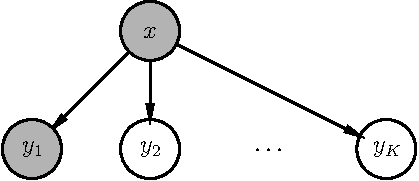
\includegraphics[width=.8\textwidth]{mmclassifier.pdf} % textwidth in subfigure environment
        \caption{Multi-class multi-label classifier}
    \end{subfigure}
    \begin{subfigure}[t]{.33\textwidth}
        \centering
        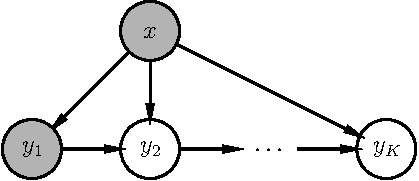
\includegraphics[width=.8\textwidth]{memm.pdf}
        \caption{MEMM}
    \end{subfigure}
    \begin{subfigure}[t]{.33\textwidth}
        \centering
        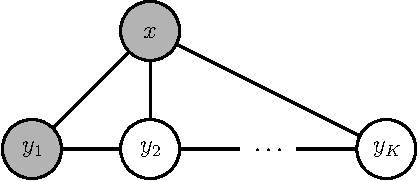
\includegraphics[width=.8\textwidth]{crf.pdf}
        \caption{CRF}
    \end{subfigure}
    \caption{Graphical models for trajectory recommendation.}
    \label{fig:pgm}
\end{figure}


\subsubsection{Maximum-entropy Markov models}
\label{sec:memm}

For MEMM, the compatibility function $f(\mathbf{x}, \mathbf{y})$ is the probability of trajectory $\mathbf{y}$ given query $\mathbf{x} = (s, K)$,
\begin{equation*}
f(\mathbf{x}, \mathbf{y}) 
= \mathbb{P}(\mathbf{y} \mid \mathbf{x}; \mathbf{w}) 
= \mathbb{P}(y_1 \mid \mathbf{x}; \mathbf{w}) \cdot \prod_{j=2}^K \mathbb{P}(y_j \mid y_{j-1}, \mathbf{x}; \mathbf{w})
= 1 \cdot \prod_{j=2}^{K}~
  \frac{\exp \left(\mathbf{w}^\top \Psi_j(\mathbf{x}, y_{j-1}, y_j) \right)}
       {\sum_{y' \in \mathcal{P}} \exp \left(\mathbf{w}^\top \Psi_j(\mathbf{x}, y_{j-1}, y') \right)},
\end{equation*}
where we do local normalisation.

The negative log-likelihood of training set is
\begin{equation*}
\ell(\mathbf{w}) 
= -\sum_{i=1}^N \log \mathbb{P}(\mathbf{y}^{(i)} \mid \mathbf{x}^{(i)}; \mathbf{w}) \\
= -\sum_{i=1}^N \sum_{j=2}^{\mid \mathbf{y}^{(i)} \mid} 
                \mathbf{w}^\top \Psi_j(\mathbf{x}^{(i)}, y_{j-1}^{(i)}, y_j^{(i)}) +
   \sum_{i=1}^N \sum_{j=2}^{\mid \mathbf{y}^{(i)} \mid} 
                \log \sum_{y' \in \mathcal{P}} \exp \left(\mathbf{w}^\top \Psi_j(\mathbf{x}^{(i)}, y_{j-1}^{(i)}, y') \right).
\end{equation*}

To learn the parameters, we maximise the likelihood of training set by minimising its negative log-likelihood (with L2 regularisation)
\begin{equation}
\label{eq:trainmemm}
\min_{\mathbf{w}} \frac{1}{2} \mathbf{w}^\top \mathbf{w} + C \ell(\mathbf{w}).
\end{equation}

A straightforward approach to optimise the above objective is employing gradient descent. 
Let $J(\mathbf{w})$ be the objective (cost function), i.e.,
\begin{align*}
J(\mathbf{w}) 
&= \frac{1}{2} \mathbf{w}^\top \mathbf{w} + C \ell(\mathbf{w}) \\
&= \frac{1}{2} \mathbf{w}^\top \mathbf{w} -
   C \sum_{i=1}^N \sum_{j=2}^{\mid \mathbf{y}^{(i)} \mid} \mathbf{w}^\top \Psi_j(\mathbf{x}^{(i)}, y_{j-1}^{(i)}, y_j^{(i)}) +
   C \sum_{i=1}^N \sum_{j=2}^{\mid \mathbf{y}^{(i)} \mid} \log \sum_{y' \in \mathcal{P}} 
     \exp \left(\mathbf{w}^\top \Psi_j(\mathbf{x}^{(i)}, y_{j-1}^{(i)}, y') \right).
\end{align*}
The gradient of the cost function w.r.t. parameters $\mathbf{w}$ is
\begin{align*}
\frac{\partial J{\mathbf{w}}}{\partial \mathbf{w}}
&= \mathbf{w} + C \frac{\partial \ell(\mathbf{w})}{\partial \mathbf{w}} \\
&= \mathbf{w} - C \sum_{i=1}^N \sum_{j=2}^{\mid \mathbf{y}^{(i)} \mid} \Psi_j(\mathbf{x}^{(i)}, y_{j-1}^{(i)}, y_j^{(i)}) +
   C \sum_{i=1}^N \sum_{j=2}^{\mid \mathbf{y}^{(i)} \mid} 
     \frac{\sum_{y' \in \mathcal{P}} \left( \Psi_j(\mathbf{x}^{(i)}, y_{j-1}^{(i)}, y') \cdot 
           \exp \left(\mathbf{w}^\top \Psi_j(\mathbf{x}^{(i)}, y_{j-1}^{(i)}, y') \right) \right)}
          {\sum_{y' \in \mathcal{P}} \exp \left(\mathbf{w}^\top \Psi_j(\mathbf{x}^{(i)}, y_{j-1}^{(i)}, y') \right)}.
\end{align*}


MEMM is a directed graphical model (as shown in Figure~\ref{fig:pgm}(b)) which captures transitions from one POI to any other POIs simultaneously, 
in contrast, pairwise ranking (Section~\ref{sec:rank}) captures only pairwise relations independently.

To make a prediction, we need to do a MAP inference (which can be done using the Viterbi algorithm if duplicated POIs are permitted)
\begin{equation}
\label{eq:testmemm}
\begin{aligned}
\mathbf{y}^* 
&= \argmax_{\mathbf{y} \in \mathcal{Y}_\mathbf{x}}~f(\mathbf{x}, \mathbf{y})
 = \argmax_{\mathbf{y} \in \mathcal{Y}_\mathbf{x}}~\mathbb{P}(\mathbf{y} \mid \mathbf{x}; \mathbf{w})
 = \argmax_{\mathbf{y} \in \mathcal{Y}_\mathbf{x}}~\log \mathbb{P}(\mathbf{y} \mid \mathbf{x}; \mathbf{w}) \\
&= \argmax_{\mathbf{y} \in \mathcal{Y}_\mathbf{x}}~\sum_{j=2}^{K} \mathbf{w}^\top \Psi_j(\mathbf{x}, y_{j-1}, y_j) - 
   \sum_{j=2}^{K} \log \sum_{y' \in \mathcal{P}} \exp \left(\mathbf{w}^\top \Psi_j(\mathbf{x}, y_{j-1}, y') \right).
\end{aligned}
\end{equation}

Furthermore, we can explicitly model dependencies between POIs in trajectory by adding dependences between variable $y_j$ and $y_k,~ j < k$,
which results in another compatibility function
\begin{equation*}
f(\mathbf{x}, \mathbf{y}) 
= \mathbb{P}(\mathbf{y} \mid \mathbf{x}; \mathbf{w}) 
= \mathbb{P}(y_1 \mid \mathbf{x}; \mathbf{w}) \cdot \prod_{j=2}^K \mathbb{P}(y_j \mid y_1,\dots, y_{j-1}, \mathbf{x}; \mathbf{w})
= 1 \cdot \prod_{j=2}^{K}~
  \frac{\exp \left(\mathbf{w}_j^\top \Psi_j(\mathbf{x}, y_1, \dots, y_{j-1}, y_j) \right)}
       {\sum_{y' \in \mathcal{P}} \exp \left(\mathbf{w}_j^\top \Psi_j(\mathbf{x}, y_1, \dots, y_{j-1}, y') \right)}.
\end{equation*}

It can be trained similarly using the maximum likelihood principle.



\subsubsection{Conditional random fields}
\label{sec:crf}

For linear chain CRF, the compatibility function $f(\mathbf{x}, \mathbf{y})$ is also the probability of trajectory $\mathbf{y}$ given
query $\mathbf{x} = (s, K)$,
\begin{equation*}
f(\mathbf{x}, \mathbf{y}) = \mathbb{P}(\mathbf{y} \mid \mathbf{x}; \mathbf{w}) 
= \frac{\exp \left( \mathbf{w}^\top \Psi(\mathbf{x}, \mathbf{y}) \right)}
       {\sum_{\mathbf{y}' \in \mathcal{Y}_\mathbf{x}} \exp \left( \mathbf{w}^\top \Psi(\mathbf{x}, \mathbf{y}') \right)}
= \frac{\prod_{j=2}^{K} \exp \left( \mathbf{w}_j^\top \Psi_j(\mathbf{x}, y_{j-1}, y_j) \right)}
       {\sum_{\mathbf{y}' \in \mathcal{Y}_\mathbf{x}} \prod_{j=2}^{K} \exp \left( \mathbf{w}_j^\top \Psi_j(\mathbf{x}, y_{j-1}', y_j') \right)},
\end{equation*}
where $\mathbf{y} \in \mathcal{Y}_\mathbf{x}$ and we assume decomposition 
$\mathbf{w}^\top \Psi(\mathbf{x}, \mathbf{y}) = \sum_{j=2}^{K} \mathbf{w}_j^\top \Psi_j(\mathbf{x}, y_{j-1}, y_j)$.
The denominator is known as the \emph{partition function} and we do global normalisation.

The negative log-likelihood of training set is
\begin{equation*}
\ell(\mathbf{w}) 
= -\sum_{i=1}^N \log \mathbb{P}(\mathbf{y}^{(i)} \mid \mathbf{x}^{(i)}; \mathbf{w})
= -\sum_{i=1}^N \sum_{j=2}^{\mid \mathbf{y}^{(i)} \mid} \mathbf{w}_j^\top \Psi_j(\mathbf{x}^{(i)}, y_{j-1}^{(i)}, y_j^{(i)}) +
   \sum_{i=1}^N \log \sum_{\mathbf{y}' \in \mathcal{Y}_\mathbf{x}} 
                \prod_{j=2}^{K} \exp \left(\mathbf{w}_j^\top \Psi_j(\mathbf{x}^{(i)}, y_{j-1}', y_j')\right).
\end{equation*}

To learn the parameters, we maximise the likelihood of training set by minimising its negative log-likelihood (with L2 regularisation)
\begin{equation}
\label{eq:traincrf}
\min_{\mathbf{w}} \frac{1}{2} \mathbf{w}^\top \mathbf{w} + C \ell(\mathbf{w}).
\end{equation}

CRF is an undirected graphical model as shown in Figure~\ref{fig:pgm}(c).
Similar to MEMM, CRF can capture transitions from one POI to any other POIs simultaneously.
To make a prediction, we need to do a MAP inference
\begin{equation}
\label{eq:testcrf}
\begin{aligned}
\mathbf{y}^* 
&= \argmax_{\mathbf{y} \in \mathcal{Y}_\mathbf{x}}~f(\mathbf{x}, \mathbf{y})
 = \argmax_{\mathbf{y} \in \mathcal{Y}_\mathbf{x}}~\mathbb{P}(\mathbf{y} \mid \mathbf{x}; \mathbf{w})
 = \argmax_{\mathbf{y} \in \mathcal{Y}_\mathbf{x}}~\log \mathbb{P}(\mathbf{y} \mid \mathbf{x}; \mathbf{w}) \\
&= \argmax_{\mathbf{y} \in \mathcal{Y}_\mathbf{x}}~\sum_{j=2}^{K} \mathbf{w}_j^\top \Psi_j(\mathbf{x}, y_{j-1}, y_j) -
   \log \sum_{\mathbf{y}' \in \mathcal{Y}_\mathbf{x}} \prod_{j=2}^{K} \exp \left( \mathbf{w}_j^\top \Psi_j(\mathbf{x}, y_{j-1}', y_j') \right).
\end{aligned}
\end{equation}

\eat{TODO: why people usually employ CRF?}


\subsubsection{Structured SVM}
\label{sec:ssvm}

For structured SVM, the compatibility function $f(\mathbf{x}, \mathbf{y})$ is this linear form,
\begin{equation*}
f(\mathbf{x}, \mathbf{y}) = \mathbf{w}^\top \Psi(\mathbf{x}, \mathbf{y}),
\end{equation*}
where $\Psi(\mathbf{x}, \mathbf{y})$ is a \emph{joint feature map} 
that captures features extracted from both query $\mathbf{x}$ and trajectory $\mathbf{y}$.

The design of joint feature $\Psi(\cdot,\cdot)$ is problem specific, 
for trajectory recommendation, we assume decomposition
\begin{equation*}
\label{eq:jointfeature}
\mathbf{w}^\top \Psi(\mathbf{x}, \mathbf{y}) 
= \sum_{j=2}^{\mid \mathbf{y} \mid} 
  \left( \mathbf{w}_j^\top \Psi_j(\mathbf{x}, y_j) + 
  \mathbf{w}_{j-1,j}^\top \Psi_{j-1, j}(\mathbf{x}, y_{j-1}, y_j) \right),
\end{equation*}
where $\Psi_j$ is a feature vector of POI $y_j$ (w.r.t. query $\mathbf{x}$)
and $\Psi_{j-1,j}$ is a pairwise feature vector that captures the affinity of transition from POI $y_{j-1}$ to POI $y_j$.

To learn the parameters, we train the structured SVM by optimising a quadratic program (QP),
\begin{equation}
\label{eq:nslack}
\begin{aligned}
\min_{\mathbf{w}, ~\bm{\xi} \ge 0} ~& \frac{1}{2} \mathbf{w}^\top \mathbf{w} + \frac{C}{n} \sum_{i=1}^n \xi_i \\
s.t.~~ ~& \mathbf{w}^\top \Psi(\mathbf{x}^{(i)}, \mathbf{y}^{(i)}) - \mathbf{w}^\top \Psi(\mathbf{x}^{(i)}, \bar{\mathbf{y}}) \ge 
       \Delta(\mathbf{y}^{(i)}, \bar{\mathbf{y}}) - \xi_i, ~\bar{\mathbf{y}} \in \mathcal{Y}_{\mathbf{x}^{(i)}},~\forall i,
\end{aligned}
\end{equation}
where $\Delta(\mathbf{y}, \bar{\mathbf{y}})$ is a discrepancy function that measures the loss 
for predicting $\bar{\mathbf{y}}$ given ground truth $\mathbf{y}$, 
and slack variable $\xi_i$ is the \emph{hinge loss} for the prediction of the $i$-th example~\cite{tsochantaridis2005large},
\begin{equation*}
\xi_i = \max \left( 0,~ 
        \max_{\bar{\mathbf{y}} \in \mathcal{Y}_{\mathbf{x}^{(i)}}} 
        \left\{ \Delta(\mathbf{y}^{(i)}, \bar{\mathbf{y}}) + \mathbf{w}^\top \Psi(\mathbf{x}^{(i)}, \bar{\mathbf{y}}) \right\} -
        \mathbf{w}^\top \Psi(\mathbf{x}^{(i)}, \mathbf{y}^{(i)}) \right).
\end{equation*}
%This formulation is called "$n$-slack" as we have one slack variable for each example in training set.

We can rewrite the constraint in problem (\ref{eq:nslack}) as
\begin{equation}
\label{eq:ssvminf}
\mathbf{w}^\top \Psi(\mathbf{x}^{(i)}, \mathbf{y}^{(i)}) + \xi_i \ge
          \max_{\bar{\mathbf{y}} \in \mathcal{Y}_{\mathbf{x}^{(i)}}}
          \left\{\mathbf{w}^\top \Psi(\mathbf{x}^{(i)}, \bar{\mathbf{y}}) + \Delta(\mathbf{y}^{(i)}, \bar{\mathbf{y}}) \right\},~ \forall i,
\end{equation}
where the right hand side is known as the \emph{loss-augmented inference}.

To solve problem (\ref{eq:nslack}), one option is simply enumerating all constraints, and feeding the problem into a standard QP solver.
However, this approach is impractical as there is a constraint for every possible label $\bar{\mathbf{y}}$.
Instead, we use a cutting-plane algorithm which repeatedly solves QP (\ref{eq:nslack}) 
w.r.t. different set of constraints~\cite{joachims2009predicting}.
In each iteration, a new constraint is formed by solving the loss-augmented inference, 
which helps shrink the feasible region of the problem.



\subsubsection{Discussion}

All structured models described above suffer from a number of drawbacks.
\begin{enumerate}
\item The MEMM model (Section~\ref{sec:memm}) is relatively easy to train, 
      but the inference (Equation~\ref{eq:testmemm}) will not retain its efficiency if the no duplicates constraints are required.
\item The CRF model (Section~\ref{sec:crf}) suffers from inefficient training (Equation~\ref{eq:traincrf}) and 
      inference (Equation~\ref{eq:testcrf}) as the partition function cannot be computed efficiently.
\item Both the loss-augmented inference and prediction inference for structured SVM (Section~\ref{sec:ssvm}) cannot be done efficiently 
      if the no duplicates constraints are required.
\end{enumerate}

Approximate inference methods are critical for MEMM and CRF.
On the other hand, inference in structured SVM is equivalent to 
find a maximum-weight loop-less path with exactly $K$ edges in a complete weighted (both nodes and edges) graph, which is NP-hard (proof?).
Possible solutions including 
\begin{itemize}
\item formulating it as an integer linear program (ILP) and solve it using an ILP solver, 
      or using lazy constraint generation/cutting-plane techniques with a LP solver;
\item in addition, we can employ the list Viterbi algorithm~\cite{nilsson2001sequentially,seshadri1994list} 
      which sequentially find the next best (scored) trajectory until a maximum-weight loop-less path with exactly $K$ edges is found;
\item moreover, we can employ heuristics such as greedy search or the Christofides algorithm~\cite{christofides1976} 
      when the problem has the triangle inequality property (for trajectories, indeed).
\end{itemize}
These options are applicable to MEMM (Section~\ref{sec:memm}) as well.



\subsubsection{Inference algorithms}
\label{sec:inference}

\paragraph{Integer linear program}
If we formulate an ILP to do inference and employ the sub-tour elimination constraints from TSP, we have
\begin{alignat}{5}
& \max_{u,v} ~&& \sum_{k=1}^M \mathbf{w}_k^\top \phi_k(\mathbf{x}, p_k) \sum_{j=1}^M u_{jk} + 
                 \sum_{j=1}^M \sum_{k=1}^M u_{jk} \mathbf{w}_{jk}^\top \phi_{j, k}(\mathbf{x}, p_j, p_k) \\
& s.t. ~~ ~&& u_{jk}, ~z_j \in \{0, 1\}, ~u_{jj}=0, ~z_1=0, ~v_j \in \mathbf{Z},~ p_j \in \mathcal{P}, ~\forall j, k = 1,\cdots,M   \label{eq:cons1} \\
&          && \sum_{k=2}^M u_{1k} = 1, ~\sum_{j=2}^M u_{j1} = 0  \label{eq:cons2} \\
&          && \sum_{j=1}^M u_{jl} = z_l + \sum_{k=2}^M u_{lk} \le 1,   ~\forall l=2,\cdots,M                    \label{eq:cons3} \\
&          && \sum_{j=1}^M \sum_{k=1}^M u_{jk} = L-1,                                                           \label{eq:cons4} \\
&          && v_j - v_k + 1 \le (M-1) (1-u_{jk}),                     \forall j,k=2,\cdots,M                    \label{eq:cons5}
\end{alignat}
where $u_{jk}$ is a binary decision variable that determines whether the transition from $p_j$ to $p_k$ is in the resulting trajectory,
$z_j$ is a binary decision variable that determines whether $p_j$ is the last POI in trajectory.
$L$ is the number of POIs in trajectory.
For brevity, we arrange the POIs such that $p_1 = s$.
Firstly, the desired trajectory should start from $s$ (Constraint~\ref{eq:cons2}).
In addition, any POI could be visited at most once (Constraint~\ref{eq:cons3}).
Moreover, only $L-1$ transitions between POIs are permitted (Constraint~\ref{eq:cons4}),
i.e., the number of POI visits should be exactly $L$ (including $s$).
The last constraint, where $v_i$ is an auxiliary variable,
enforces that only a single sequence of POIs without sub-tours is permitted in the trajectory.

If we employ the above ILP to do loss-augmented inference, we can simply add a linear loss function to the objective, 
e.g., $\Delta(\mathbf{y}, \bar{\mathbf{y}}) = 1 - \sum_{j=1}^M \sum_{k=1}^M u_{j, y_k}$ if we define the loss as the number of mispredicted POIs,
where $\mathbf{y}$ is the ground truth and $\bar{\mathbf{y}}$ is the trajectory corresponding to the optimal solution of this ILP.

\paragraph{The list Viterbi algorithm}
Instead of employ an algorithm with exponential time complexity (e.g., ILP) to do inference,
we can resort to an iterative algorithm such as the list Viterbi algorithm~\cite{nilsson2001sequentially,seshadri1994list}
which sequentially find the $k$-th best (scored) trajectory given the best, $2$nd best, \dots, $(k-1)$-th best (scored) trajectories,
as described in Algorithm~\ref{alg:listviterbi}.


\begin{algorithm}[htbp]
\caption{The list Viterbi algorithm for inference}
\label{alg:listviterbi}
\begin{algorithmic}[1]
\STATE \textbf{Input}: $\mathbf{x}=(s, K),~ \mathcal{P},~ \mathbf{w},~ \Psi$
\STATE Initialise score matrices $\alpha,~ \beta,~ f_t,~ f_{t, t+1}$, a max-heap $H,~ k=0$.
\STATE $\triangleright$ Do the forward-backward procedure~\cite{rabiner1989tutorial}
\STATE $\forall p_j \in \mathcal{P},~ \alpha_t(p_j) = 
        \begin{cases}
        0,~ t = 1 \\
        \max_{p_i \in \mathcal{P}} \left\{ \alpha_{t-1}(p_i) + \mathbf{w}_{ij}^\top \Psi_{ij}(\mathbf{x}, p_i, p_j) + 
        \mathbf{w}_j^\top \Psi_j(\mathbf{x}, p_j) \right\},~ t=2,\dots,K
        \end{cases}$

\STATE $\forall p_i \in \mathcal{P},~ \beta_t(p_i) = 
        \begin{cases}
        0,~ t = K \\
        \max_{p_j \in \mathcal{P}} \left\{ \mathbf{w}_{ij}^\top \Psi_{ij}(\mathbf{x}, p_i, p_j) + 
        \mathbf{w}_j^\top \Psi_j(\mathbf{x}, p_j) + \beta_{t+1}(p_j) \right\},~ t = K-1,\dots,1
        \end{cases}$

\STATE $\forall p_i \in \mathcal{P},~ f_t(p_i) = \alpha_t(p_i) + \beta_t(p_i),~ t = 1,\dots,K$
\STATE $\forall p_i, p_j \in \mathcal{P},~ f_{t,t+1}(p_i, p_j) = \alpha_t(p_i) + \mathbf{w}_{ij}^\top \Psi_{ij}(\mathbf{x}, p_i, p_j) + 
                              \mathbf{w}_j^\top \Psi_j(\mathbf{x}, p_j) + \beta_{t+1}(p_j),~ t = 1,\dots,K-1$

\STATE $\triangleright$ Identify the best (scored) trajectory $\mathbf{y}^1=(y_1^1,\dots,y_K^1)$ (possibly with sub-tours)
\STATE $y_t^1 = \begin{cases}
                s,~ t = 1 \\
%                \argmax_{p \in \mathcal{P}} \left\{ f_{1,2}(s, p) \right\},~ t = 2, \\
                \argmax_{p \in \mathcal{P}} \left\{ f_{t-1,t}(y_{t-1}^1, p) \right\},~ t = 2,\dots,K
                \end{cases}$

\STATE $r^1 = \max_{p \in \mathcal{P}} \left\{ f_K(p) \right\}~~~ \triangleright$ $r^1$ is the score/priority of $\mathbf{y}^1$
\STATE $H.\textit{push}\left(r^1,~ (\mathbf{y}^1, \textsc{nil}, \emptyset) \right)$

\WHILE{$H \ne \emptyset$ \textbf{and} $k < \,\mid\!\!\mathcal{P}\!\!\mid^{K-1} - \prod_{t=2}^K (\mid\!\!\mathcal{P}\!\!\mid-t+1)$}
    \STATE $r^k,~ (\mathbf{y}^k, I, S) = H.\textit{pop}()~~~ \triangleright$ 
           $r^k$ is the score of $\mathbf{y}^k=(y_1^k,\dots,y_K^k)$, $I$ is the partition index, and $S$ is the exclude set
    \STATE $k = k + 1$
    \RETURN $\mathbf{y}^k$ if NO sub-tours in $\mathbf{y}^k$
    \STATE $\bar{I} = \begin{cases}
                      2,~ I = \textsc{nil} \\
                      I,~ \text{otherwise}
                      \end{cases}$

    \FOR{$t = \bar{I},\dots,K$}
        \STATE $\bar{S} = \begin{cases}
                          S \cup \{ y_t^k \},~ t = \bar{I} \\
                          \{ y_t^k \},~ \text{otherwise}
                          \end{cases}$

        \STATE $\bar{y}_j = \begin{cases}
                            y_j^k,~~ j=1,\dots,t-1 \\
                            %\argmax_{p \in \mathcal{P} \setminus \textit{new\_exclude\_set}} f_{t-1,t}(y_{t-1}^k, p),~ j=t \\
                            \argmax_{p \in \mathcal{P} \setminus \bar{S}} \left\{ f_{t-1,t}(y_{t-1}^k, p) \right\},~ j=t \\
                            \argmax_{p \in \mathcal{P}} \left\{ f_{j-1, j}(\bar{y}_{j-1}, p) \right\},~ j=t+1,\dots,K
                \end{cases}$
        \STATE $\bar{r} = \begin{cases}
                          f_{t-1,t}(y_{t-1}^k, \bar{y}_t),~ I = \textsc{nil} \\
                          r^k + f_{t-1,t}(y_{t-1}^k, \bar{y}_t) - f_{t-1,t}(y_{t-1}^k, y_t^k),~ \text{otherwise}
                          \end{cases}$

        $H.\textit{push}\left(\bar{r}, (\bar{\mathbf{y}}, t, \bar{S}) \right)$
    \ENDFOR
\ENDWHILE
\end{algorithmic}
\end{algorithm}



\eat{
\subsection{Other models}
\label{sec:other}
Label ranking model,
Plackett-Luce probabilistic ranking
}


\section{Features}
\label{sec:feature}

\eat{
\underline{REVISE FEATURE DESIGN}
}

The POI and query specific features extracted from trajectories are shown in Table~\ref{tab:poifeature},
features that describe the transition preference between different POIs are shown in Table~\ref{tab:tranfeature}.



\begin{table*}[ht]
\caption{Features of POI $p$ with respect to query $(s,K)$}
\label{tab:poifeature}
\centering
\setlength{\tabcolsep}{10pt} % tweak the space between columns
\begin{tabular}{l|l} \hline
\textbf{Feature}  & \textbf{Description} \\ \hline
\texttt{category}               & one-hot encoding of the category of $p$ \\
\texttt{neighbourhood}          & one-hot encoding of the POI cluster that $p$ resides in \\
\texttt{popularity}             & logarithm of POI popularity of $p$ \\
\texttt{nVisit}                 & logarithm of the total number of visit by all users at $p$ \\
\texttt{avgDuration}            & logarithm of the average duration at $p$ \\ \hline

%\texttt{nOccurrence}            & the number of times $p$ occurred in a trajectory that satisfies the query \\ DON'T know given new query

\texttt{trajLen}                & trajectory length $K$, i.e., the number of POIs required \\
\texttt{sameCatStart}           & $1$ if the category of $p$ is the same as that of $s$, $-1$ otherwise \\
\texttt{sameNeighbourhoodStart} & $1$ if $p$ resides in the same POI cluster as $s$, $-1$ otherwise \\
\texttt{distStart}              & distance between $p$ and $s$, calculated using the Haversine formula \\
\texttt{diffPopStart}           & real-valued difference in POI popularity of $p$ from that of $s$ \\
\texttt{diffNVisitStart}        & real-valued difference in the total number of visit at $p$ from that at $s$ \\
\texttt{diffDurationStart}      & real-valued difference in average duration at $p$ from that at $s$ \\
\hline
\end{tabular}
\end{table*}



\begin{table}[ht]
\caption{POI features used to estimate the (feature-wise) transition probabilities}
\label{tab:tranfeature}
\centering
%\setlength{\tabcolsep}{28pt} % tweak the space between columns
\begin{tabular}{l|l} \hline
\textbf{Feature}       & \textbf{Description} \\ \hline
\texttt{category}      & category of POI \\
\texttt{neighbourhood} & the cluster that a POI resides in \\
\texttt{popularity}    & (discretised) popularity of POI \\
\texttt{nVisit}        & (discretised) total number of visit at POI \\
\texttt{avgDuration}   & (discretised) average duration at POI \\ \hline
\end{tabular}
\end{table}


%\section{Problem formulation}
\label{sec:formulation}

The trajectory recommendation problem is: given a set of points-of-interest (POI) $\mathcal{P}$ and a trajectory query $\mathbf{x} = (s, K)$,
where $s \in \mathcal{P}$ is the desired start POI and $K > 1$ is the number of POIs in the desired trajectory (including the start location $s$).
We want to recommend a sequence of POIs $\mathbf{y}^*$ that maximises utility, i.e., for a suitable function $f(\cdot,\cdot)$,
\begin{equation*}
\mathbf{y}^* = \argmax_{\mathbf{y} \in \mathcal{Y}_\mathbf{x}}~f(\mathbf{x}, \mathbf{y}),
\end{equation*}
where $\mathcal{Y}_\mathbf{x}$ is the set of all possible trajectories with POIs in $\mathcal{P}$ and satisfying query $\mathbf{x}$.
$\mathbf{y} = (y_1 = s,~ y_2, \dots, y_K)$ is a trajectory with $K$ POIs, and $y_j \ne y_k$ if $j \ne k$ 
which is known as \emph{no duplicates constraint}.

Instead of the number of desired POIs, we can constrain the trajectory with a total time budget $T$.
In this case, the number of POIs $K$ can be treated as a \emph{hidden} variable, with additional constraint $\sum_{k=1}^K t_k \le T$ 
where $t_k$ is the time spent at POI $y_k$.



\subsection{A concrete example}
\label{sec:example}

Given a set of $10$ points-of-interest (POI) in Melbourne 
\begin{align*}
\mathcal{P} = \{ 
& \textit{\small Eureka Tower, Federation Square, Flinders Street Railway Station, Luna Park, Melbourne Aquarium, Melbourne Cricket Ground,} \\
& \textit{\small Melbourne Zoo, National Gallery of Victoria, Royal Exhibition Building, University of Melbourne} \}
\end{align*}
and a query $\mathbf{x} = \{\textit{\small University of Melbourne},~ 5\}$,
we would like to recommend a trajectory 
\begin{equation*}
\mathbf{y} = \{\textit{\small University of Melbourne},~ y_2, \dots, y_5\},~ y_k \in \mathcal{P},~ k=2,\dots,5.
\end{equation*}
by modelling trajectory data we have with POI and query related features as described in Section~\ref{sec:feature}.



\subsection{Related problems}
\label{sec:related}

This problem is related to automatic playlist generation, 
where we recommend a sequence of songs given a specified song (a.k.a. the seed) and the number of new songs.
Formally, given a library of songs and a query $\mathbf{x} = (s, K)$, where $s$ is the seed and $K$ is the number of songs in playlist,
we produce a list with $K$ songs (without duplication) by maximising the likelihood~\cite{chen2012playlist},
\begin{equation*}
%\max_{(y_1,\dots,y_K)} \prod_{k=2}^K \mathbb{P}(y_{k-1} \mid y_k),~ y_1 = s ~\text{and}~ y_j \ne y_k,~ j \ne k.
\mathbf{y}^* = \argmax_{\mathbf{y} \in \mathcal{P}_\mathbf{x}}~ \mathbb{P}(\mathbf{y} \mid \mathbf{x}),~ \mathbf{y} = (y_1=s,\dots,y_K) 
~\text{and}~ y_j \ne y_k ~\text{if}~ j \ne k.
\end{equation*}

Another similar problem is choosing a small set of photos from a large photo library and compiling them into a slideshow or movie.



\subsection{Evaluation metrics and loss functions}
\label{sec:evaluation}

To evaluate the performance of a certain recommendation algorithm,
we need to measure the similarity (or loss) given prediction $\hat{\mathbf{y}}$ and ground truth $\mathbf{y}$.
Metrics researchers have used include
\begin{itemize}
\item Hamming loss $\frac{1}{K} \sum_{j=1}^K \llb \hat{y}_j \neq y_j \rrb$, this checks if every position is the same.

\item F$_1$ score on points~\cite{ijcai15}, where we care about the set of correctly recommended POIs. 
      Let $\texttt{set}(\mathbf{y})$ denote the set of POIs in trajectory $\mathbf{y}$, F$_1$ score on points is defined as
\begin{equation*}
F_1 = \frac{2  P_{\textsc{point}}  R_{\textsc{point}}}{P_{\textsc{point}} + R_{\textsc{point}}} ~~\text{where}~
P_{\textsc{point}} = \frac{\mid \texttt{set}(\hat{\mathbf{y}}) \cap \texttt{set}(\mathbf{y}) \mid}{\mid \texttt{set}(\hat{\mathbf{y}}) \mid}~\text{and}~
R_{\textsc{point}} = \frac{\mid \texttt{set}(\hat{\mathbf{y}}) \cap \texttt{set}(\mathbf{y}) \mid}{\mid \texttt{set}(\mathbf{y}) \mid}.
\end{equation*}
If $\mid\!\! \hat{\mathbf{y}} \!\!\mid = \mid\!\! \mathbf{y} \!\!\mid$, this metric is just the unordered Hamming loss, 
i.e., Hamming loss between two binary indicator vectors of size $\mid\!\! \mathcal{P} \!\!\mid$.


\item F$_1$ score on pairs~\cite{cikm16paper}, where we care about the set of correctly predicted POI pairs,
\begin{equation*}
\text{pairs-F}_1 = \frac{2 P_{\textsc{pair}} R_{\textsc{pair}}}{P_{\textsc{pair}} + R_{\textsc{pair}}}~~\text{where}~
P_{\textsc{pair}} = \frac{N_c} {\mid \texttt{set}(\hat{\mathbf{y}}) \mid (\mid \texttt{set}(\hat{\mathbf{y}}) \mid - 1) / 2}~\text{and}~
R_{\textsc{pair}} = \frac{N_c} {\mid \texttt{set}(\mathbf{y}) \mid (\mid \texttt{set}(\mathbf{y}) \mid - 1) / 2},
\end{equation*}
and $N_c = \sum_{j=1}^{\mid \mathbf{y} \mid - 1} \sum_{k=j+1}^{\mid \mathbf{y} \mid} \llb y_j \prec_{\bar{\mathbf{y}}} y_k \rrb$,
here $y_j \prec_{\bar{\mathbf{y}}} y_k$ denotes that POI $y_j$ appears before POI $y_k$ in trajectory $\bar{\mathbf{y}}$.
We define pairs-F$_1 = 0$ when $N_c = 0$.

\end{itemize}

However, if we cast a trajectory $\mathbf{y} = (y_1,\dots,y_K)$ as a ranking of POIs in $\mathcal{P}$,
where $y_k$ has a rank $\mid\!\! \mathcal{P} \!\!\mid\! - k + 1$ and any other POI $p \notin \mathbf{y}$ has a rank $0$ ($0$ is an arbitrary choice).
We can make use of ranking evaluation metrics such as Kendall's $\tau$ or Spearman's $\rho$, by taking care of ties in ranks.

\eat{TODO: Write these down and contrast, esp. to pairs-F1}.



\subsection{Kendall's $\tau$}
\label{sec:kendalltau}

Given two ranks $X$ and $Y$, each with $n$ observations, we define
\begin{itemize}
\item Number of concordant pairs 
      \begin{equation*}
      %C = \sum_{i < j} \left( \mathbbm{1}(X_i < X_j) \cdot \mathbbm{1}(Y_i < Y_j) + \mathbbm{1}(X_i > X_j) \cdot \mathbbm{1}(Y_i > Y_j) \right),
      C = \frac{1}{2} \sum_{i,j} \left( \llb X_i < X_j \rrb \cdot \llb Y_i < Y_j \rrb + \llb X_i > X_j \rrb \cdot \llb Y_i > Y_j \rrb \right),
      \end{equation*}
      where $\llb \cdot \rrb$ is the indicator function and 
      $\sum_{i,j}$ means all ordered pairs $(i, j),~ i,j=1,\dots,n$ are counted twice.

\item Number of discordant pairs 
      \begin{equation*}
      D = \frac{1}{2} \sum_{i,j} \left( \llb X_i < X_j \rrb \cdot \llb Y_i > Y_j \rrb + \llb X_i > X_j \rrb \cdot \llb Y_i < Y_j \rrb \right).
      \end{equation*}

\item Number of ties in $X$
      \begin{equation*}
      T_X = \frac{1}{2} \sum_{i \ne j} \llb X_i = X_j \rrb = \sum_k \frac{t_k (t_k - 1)}{2},
      \end{equation*}
      where $t_k$ is the number of tied values in the $k$-th group of ties for $X$, for example, if
      $X = [12, 2, 1, 12, 2, 2, 1]$, there are $3$ groups of tied values, the first group is the two $12$'s, i.e., $t_1 = 2$;
      the second group is the three $2$'s, i.e., $t_2 = 3$; the third group is the two $1$'s, i.e., $t_3 = 2$. \\
      Similarly, the number of ties in $Y$ is 
      \begin{equation*}
      T_Y = \frac{1}{2} \sum_{i \ne j} \llb Y_i = Y_j \rrb = \sum_k \frac{u_k (u_k - 1)}{2},
      \end{equation*}
      where $u_k$ is the number of tied values in the $k$-th group of ties for $Y$.

\item Number of ties in both $X$ and $Y$
      \begin{equation*}
      T_{XY} = \frac{1}{2} \sum_{i \ne j} \llb X_i = X_j \rrb \cdot \llb Y_i = Y_j \rrb.
      \end{equation*}

\item Number of ties only in $X$
      \begin{equation*}
      T = \frac{1}{2} \sum_{i \ne j} \llb X_i = X_j \rrb \cdot \llb Y_i \ne Y_j \rrb,
      \end{equation*}
      and the number of ties only in $Y$
      \begin{equation*}
      U = \frac{1}{2} \sum_{i \ne j} \llb X_i \ne X_j \rrb \cdot \llb Y_i = Y_j \rrb.
      \end{equation*}
\end{itemize}

Kendall's $\tau$ (version $b$) is defined as~\cite{kendall1945,agresti2010analysis} (and implemented in SciPy~\cite{scipy})
\begin{equation*}
\tau_b = \frac{C - D}{\sqrt{[n(n-1)/2 - T_X] [n(n-1)/2 - T_Y]}} = \frac{C - D}{\sqrt{(C + D + T) (C + D + U)}},
\end{equation*}
where we use equalities 
\begin{align*}
\frac{n(n-1)}{2} &= C + D + T_X + T_Y - T_{XY} \\
T &= T_X - T_{XY} \\
U &= T_Y - T_{XY}
\end{align*}



\subsection{Compare Kendall's $\tau$ with F$_1$ score on points and pairs}
\label{sec:metriccomparison}

Given a prediction $\hat{\mathbf{y}} = (\hat{y}_1, \hat{y}_2, \dots, \hat{y}_K)$ and ground truth $\mathbf{y} = (y_1, y_2, \dots, y_K)$,
for a specific ordering of POIs $(p_1, p_2, \dots, p_{\mid\mathcal{P}\mid})$,
we produce two ranks according to $\mathbf{y}$ and $\hat{\mathbf{y}}$,
\begin{align*}
r_{\mathbf{y}}^i       &= \sum_{j=1}^K (\mid\!\! \mathcal{P} \!\!\mid - j + 1) \cdot \llb p_i = y_j \rrb,~
i = 1, \dots, \mid\!\! \mathcal{P} \!\!\mid \\
r_{\hat{\mathbf{y}}}^i &= \sum_{j=1}^K (\mid\!\! \mathcal{P} \!\!\mid - j + 1) \cdot \llb p_i = \hat{y}_j \rrb,~ 
i = 1, \dots, \mid\!\! \mathcal{P} \!\!\mid
\end{align*}
where POIs not in $\mathbf{y}$ will have a rank of $0$ in $r_{\mathbf{y}}$ and similarly in $r_{\hat{\mathbf{y}}}$.
Then we have
\begin{align*}
C &= \frac{1}{2} \sum_{i,j} \left(\llb r_{\mathbf{y}}^i < r_{\mathbf{y}}^j \rrb \cdot \llb r_{\hat{\mathbf{y}}}^i < r_{\hat{\mathbf{y}}}^j \rrb +
     \llb r_{\mathbf{y}}^i > r_{\mathbf{y}}^j \rrb \cdot \llb r_{\hat{\mathbf{y}}}^i > r_{\hat{\mathbf{y}}}^j \rrb \right), \\
D &= \frac{1}{2} \sum_{i,j} \left(\llb r_{\mathbf{y}}^i < r_{\mathbf{y}}^j \rrb \cdot \llb r_{\hat{\mathbf{y}}}^i > r_{\hat{\mathbf{y}}}^j \rrb +
     \llb r_{\mathbf{y}}^i > r_{\mathbf{y}}^j \rrb \cdot \llb r_{\hat{\mathbf{y}}}^i < r_{\hat{\mathbf{y}}}^j \rrb \right), \\
T_{\mathbf{y}}       &= \frac{1}{2} \sum_{i \ne j} \llb r_{\mathbf{y}}^i = r_{\mathbf{y}}^j \rrb, \\
T_{\hat{\mathbf{y}}} &= \frac{1}{2} \sum_{i \ne j} \llb r_{\hat{\mathbf{y}}}^i = r_{\hat{\mathbf{y}}}^j \rrb, \\
T_{\mathbf{y},\hat{\mathbf{y}}} &= \frac{1}{2} \sum_{i \ne j} \llb r_{\hat{\mathbf{y}}}^i = r_{\hat{\mathbf{y}}}^j \rrb \cdot
                                   \llb r_{\mathbf{y}}^i = r_{\mathbf{y}}^j \rrb, \\
T &= T_{\mathbf{y}} - T_{\mathbf{y},\hat{\mathbf{y}}},~ U = T_{\hat{\mathbf{y}}} - T_{\mathbf{y},\hat{\mathbf{y}}}.
\end{align*}
\noindent
Kendall's $\tau$
\begin{equation*}
\tau_b = \frac{C - D}{\sqrt{(C + D + T) (C + D + U)}},
\end{equation*}
F$_1$ score on points 
\begin{equation*}
F_1 = \frac{1}{K} \sum_i \llb r_{\mathbf{y}}^i > 0 \rrb \cdot \llb r_{\hat{\mathbf{y}}}^i > 0 \rrb,
\end{equation*}
and F$_1$ score on pairs
\begin{equation*}
\text{pairs-F}_1 = \frac{\frac{1}{2} \sum_{i,j} 
                   \llb r_{\mathbf{y}}^i < r_{\mathbf{y}}^j \rrb \cdot \llb r_{\mathbf{y}}^i > 0 \rrb \cdot
                   \llb r_{\hat{\mathbf{y}}}^i < r_{\hat{\mathbf{y}}}^j \rrb \cdot \llb r_{\hat{\mathbf{y}}}^i > 0 \rrb +
                   \frac{1}{2} \sum_{i,j} 
                   \llb r_{\mathbf{y}}^i > r_{\mathbf{y}}^j \rrb \cdot \llb r_{\mathbf{y}}^j > 0 \rrb \cdot
                   \llb r_{\hat{\mathbf{y}}}^i > r_{\hat{\mathbf{y}}}^j \rrb \cdot \llb r_{\hat{\mathbf{y}}}^j > 0 \rrb}{K(K-1)/2}.
\end{equation*}

We can rewrite the number of concordant pairs as
\begin{align*}
C =& \frac{1}{2} \sum_{i,j} \left(\llb r_{\mathbf{y}}^i < r_{\mathbf{y}}^j \rrb \cdot \llb r_{\hat{\mathbf{y}}}^i < r_{\hat{\mathbf{y}}}^j \rrb +
     \llb r_{\mathbf{y}}^i > r_{\mathbf{y}}^j \rrb \cdot \llb r_{\hat{\mathbf{y}}}^i > r_{\hat{\mathbf{y}}}^j \rrb \right), \\
  =& \sum_{i < j} \llb r_{\mathbf{y}}^i < r_{\mathbf{y}}^j \rrb \cdot 
     \left( \llb r_{\mathbf{y}}^i > 0 \rrb + \llb r_{\mathbf{y}}^i = 0 \rrb \right) \cdot 
     \llb r_{\hat{\mathbf{y}}}^i < r_{\hat{\mathbf{y}}}^j \rrb \cdot
     \left( \llb r_{\hat{\mathbf{y}}}^i > 0 \rrb + \llb r_{\hat{\mathbf{y}}}^i = 0 \rrb \right) + \\
   & \sum_{i < j} \llb r_{\mathbf{y}}^i > r_{\mathbf{y}}^j \rrb \cdot 
     \left( \llb r_{\mathbf{y}}^j > 0 \rrb + \llb r_{\mathbf{y}}^j = 0 \rrb \right) \cdot
     \llb r_{\hat{\mathbf{y}}}^i > r_{\hat{\mathbf{y}}}^j \rrb \cdot
     \left( \llb r_{\hat{\mathbf{y}}}^j > 0 \rrb + \llb r_{\hat{\mathbf{y}}}^j = 0 \rrb \right) \\
  =& \sum_{i < j} \left( \uwave{\llb r_{\mathbf{y}}^i < r_{\mathbf{y}}^j \rrb \cdot \llb r_{\mathbf{y}}^i > 0 \rrb} +
            \llb r_{\mathbf{y}}^i < r_{\mathbf{y}}^j \rrb \cdot \llb r_{\mathbf{y}}^i = 0 \rrb \right) \cdot 
     \left( \uwave{\llb r_{\hat{\mathbf{y}}}^i < r_{\hat{\mathbf{y}}}^j \rrb \cdot \llb r_{\hat{\mathbf{y}}}^i > 0 \rrb} + 
            \llb r_{\hat{\mathbf{y}}}^i < r_{\hat{\mathbf{y}}}^j \rrb \cdot \llb r_{\hat{\mathbf{y}}}^i = 0 \rrb \right) + \\
   & \sum_{i < j} \left( \uwave{\llb r_{\mathbf{y}}^i > r_{\mathbf{y}}^j \rrb \cdot \llb r_{\mathbf{y}}^j > 0 \rrb} + 
            \llb r_{\mathbf{y}}^i > r_{\mathbf{y}}^j \rrb \cdot \llb r_{\mathbf{y}}^j = 0 \rrb \right) \cdot
     \left( \uwave{\llb r_{\hat{\mathbf{y}}}^i > r_{\hat{\mathbf{y}}}^j \rrb \cdot \llb r_{\hat{\mathbf{y}}}^j > 0 \rrb} + 
            \llb r_{\hat{\mathbf{y}}}^i > r_{\hat{\mathbf{y}}}^j \rrb \cdot \llb r_{\hat{\mathbf{y}}}^j = 0 \rrb \right) \\
  =& \sum_{i < j} \uwave{\llb r_{\mathbf{y}}^i < r_{\mathbf{y}}^j \rrb \cdot \llb r_{\mathbf{y}}^i > 0 \rrb \cdot
                         \llb r_{\hat{\mathbf{y}}}^i < r_{\hat{\mathbf{y}}}^j \rrb \cdot \llb r_{\hat{\mathbf{y}}}^i > 0 \rrb} +
     \sum_{i < j} \uwave{\llb r_{\mathbf{y}}^i > r_{\mathbf{y}}^j \rrb \cdot \llb r_{\mathbf{y}}^j > 0 \rrb \cdot
                         \llb r_{\hat{\mathbf{y}}}^i > r_{\hat{\mathbf{y}}}^j \rrb \cdot \llb r_{\hat{\mathbf{y}}}^j > 0 \rrb} + \\
   & \sum_{i < j} \left( \uwave{\llb r_{\mathbf{y}}^i < r_{\mathbf{y}}^j \rrb \cdot \llb r_{\mathbf{y}}^i > 0 \rrb} \cdot
                         \llb r_{\hat{\mathbf{y}}}^i < r_{\hat{\mathbf{y}}}^j \rrb \cdot \llb r_{\hat{\mathbf{y}}}^i = 0 \rrb + 
                         \llb r_{\mathbf{y}}^i < r_{\mathbf{y}}^j \rrb \cdot \llb r_{\mathbf{y}}^i = 0 \rrb \cdot 
                         \llb r_{\hat{\mathbf{y}}}^i < r_{\hat{\mathbf{y}}}^j \rrb \right) + \\ 
   & \sum_{i < j} \left( \uwave{\llb r_{\mathbf{y}}^i > r_{\mathbf{y}}^j \rrb \cdot \llb r_{\mathbf{y}}^j > 0 \rrb} \cdot
                         \llb r_{\hat{\mathbf{y}}}^i > r_{\hat{\mathbf{y}}}^j \rrb \cdot \llb r_{\hat{\mathbf{y}}}^j = 0 \rrb +
                         \llb r_{\mathbf{y}}^i > r_{\mathbf{y}}^j \rrb \cdot \llb r_{\mathbf{y}}^j = 0 \rrb \cdot
                         \llb r_{\hat{\mathbf{y}}}^i > r_{\hat{\mathbf{y}}}^j \rrb \right) \\
  =& ~\text{pairs-F}_1 \cdot \frac{K(K-1)}{2}~ + \\
   & \sum_{i < j} \left( \uwave{\llb r_{\mathbf{y}}^i < r_{\mathbf{y}}^j \rrb \cdot \llb r_{\mathbf{y}}^i > 0 \rrb} \cdot
                         \llb r_{\hat{\mathbf{y}}}^i < r_{\hat{\mathbf{y}}}^j \rrb \cdot \llb r_{\hat{\mathbf{y}}}^i = 0 \rrb + 
                         \llb r_{\mathbf{y}}^i < r_{\mathbf{y}}^j \rrb \cdot \llb r_{\mathbf{y}}^i = 0 \rrb \cdot 
                         \llb r_{\hat{\mathbf{y}}}^i < r_{\hat{\mathbf{y}}}^j \rrb \right) + \\ 
   & \sum_{i < j} \left( \uwave{\llb r_{\mathbf{y}}^i > r_{\mathbf{y}}^j \rrb \cdot \llb r_{\mathbf{y}}^j > 0 \rrb} \cdot
                         \llb r_{\hat{\mathbf{y}}}^i > r_{\hat{\mathbf{y}}}^j \rrb \cdot \llb r_{\hat{\mathbf{y}}}^j = 0 \rrb +
                         \llb r_{\mathbf{y}}^i > r_{\mathbf{y}}^j \rrb \cdot \llb r_{\mathbf{y}}^j = 0 \rrb \cdot
                         \llb r_{\hat{\mathbf{y}}}^i > r_{\hat{\mathbf{y}}}^j \rrb \right).
\end{align*}

%\section{The cutting-plane methods}
\label{sec:problem}

The goal of cutting-plane methods is to find/localise a point in a convex \textit{target set} $Z \in \mathbb{R}^n$,
or determine that $Z$ is empty in some cases. 
The method does not assume any direct access to the description of $Z$,
such as the objective and constraint functions in an optimisation problem, except through a \textit{cutting-plane oracle}.
The method generates a query point $q$ and pass it to the oracle, 
the oracle either tells us that $q \in Z$ (in which case we are done), or it returns a hyperplane which separates $q$ from $Z$.
This hyperplane is called a \textit{cutting-plane}, or \textit{cut}, since it eliminates a half-space from our search.

Cutting-plane methods are also known as \textit{localisation} methods. 
A conceptual description of cutting-plane methods is shown in Algorithm~\ref{alg:cutting-plane}.


\begin{algorithm}[htbp]
\caption{Cutting-plane algorithm}
\label{alg:cutting-plane}
\begin{algorithmic}[1]
\STATE \textbf{Given}: an initial polyhedron $\mathcal{P}_0$ that contains $Z$.
\STATE $k = 0$
\REPEAT
    \STATE Generate a query point $q^{(k+1)}$ in $\mathcal{P}_k$
    \STATE Query the oracle at $q^{(k+1)}$
    \IF{~The oracle determines that $q^{(k+1)} \in Z$~}
        \RETURN $q^{(k+1)}$
    \ELSIF{~The oracle returns a cutting-plane $a_{k+1}^\top z \le b_{k+1}$~}
        \STATE Update constraints: $\mathcal{P}_{k+1} = \mathcal{P}_k \cap \{z | a_{k+1}^\top z \le b_{k+1} \}$
    \ENDIF
    \STATE $k = k + 1$
\UNTIL{Convergence or $\mathcal{P}_{k+1} = \emptyset$}
\end{algorithmic}
\end{algorithm}


\noindent
For a convex optimisation problem with $m$ constraints,

\begin{equation}
\label{eq:cvxprob}
\begin{aligned}
\min_{z} ~& f_0(z)        & \\
s.t.~~   ~& f_i(z) \le 0, & i = 1, \dots, m
\end{aligned} 
\end{equation}
where $f_0, \dots, f_m$ are convex and differentiable, the target set $Z$ is the optimal (or $\varepsilon$-suboptimal) set.

Given a query point $q$, the oracle first checks for feasibility.
If $q$ is not feasible, this means that at least one constraint in problem (\ref{eq:cvxprob}) is violated.
Suppose constraint $f_j(z) \le 0$ is violated by $q$, then we have $f_j(q) > 0$.
In addition, as $f_j(z)$ is convex and differentiable, we have the inequality
\begin{equation}
\label{eq:funprop}
f_j(z) \ge f_j(q) + \nabla f_j(q)^\top (z - q),~ j = 0, \dots, m
\end{equation}
We conclude that if $f_j(q) + \nabla f_j(q)^\top (z - q) > 0$, then $f_j(z) > 0$, 
which violated the constraint $f_j(z) \le 0$ in problem (\ref{eq:cvxprob}).
Thus, any feasible point should satisfy the inequality
\begin{equation}
\label{eq:feacut}
f_j(q) + \nabla f_j(q)^\top (z - q) \le 0.
\end{equation}
This is called a \textit{feasibility cut} for problem (\ref{eq:cvxprob}) since it cuts away the half-space 
$\{z | f_j(q) + \nabla f_j(q)^\top (z - q) > 0 \}$ with infeasible points.
If more than one constraint is violated by $q$, we can generate a \emph{feasibility cut} for each violated constraint.

On the other hand, if $q$ is feasible, and suppose $\nabla f_0(q) \ne 0$ (otherwise $q$ is optimal and we are done),
from Equation (\ref{eq:funprop}) we have
\begin{equation*}
f_0(z) > f_0(q), \text{~if~} \nabla f_0(q)^\top (z - q) > 0.
\end{equation*}
In other words, any point that satisfies inequality $\nabla f_0(q)^\top (z - q) > 0$ has an objective value larger than $f_0(q)$ 
and hence cannot be optimal.
It follows that we can form a cutting-plane
\begin{equation}
\label{eq:objcut}
\nabla f_0(q)^\top (z - q) \le 0,
\end{equation}
which is called an \textit{objective cut} for problem (\ref{eq:cvxprob}) and 
it cuts out the half-space $\{z | \nabla f_0(q)^\top (z - q) > 0 \}$ with non-optimal points.

If we keep track of the best (smallest) objective value $f_\text{best} = f_0(q_\text{best})$ for all feasible query points during the querying, 
since the optimal point has an objective value at most $f_\text{best}$, 
we can cut away the half-space of points $\{z | f_0(z) > f_\text{best} \}$ with objective values greater than $f_\text{best}$, 
which means we add a constraint $f_0(z) \le f_\text{best}$, and considering Equation~(\ref{eq:funprop}), 
we have a deep objective cut~\cite{boydlocalization},
\begin{equation}
\label{eq:deepobjcut}
f_0(q) + \nabla f_0(q)^\top (z - q) - f_\text{best} \le 0,
\end{equation}
where $q$ is the current query point. If $q = q_\text{best}$, this cut reduces to the objective cut~(\ref{eq:objcut}).

%If $q$ is feasible and $\nabla f_0(q) = 0$ then $q$ is optimal.
For non-differentiable problems, the gradients $\nabla f_j(z)$ can generally be replaced by sub-gradients.


\subsection{Generate query points}
\label{sec:query}

We would like to generate a query point $q^{(k+1)}$ in the current polyhedron $\mathcal{P}_{k}$ such that 
the resulting cut reduces the size of $\mathcal{P}_{k+1}$ as much as possible.
However, when we query the oracle at point $q^{(k+1)}$, we do not know in which direction the generated cut will be excluded.
If we measure the informativeness of the $k$-th cut using the volume reduction ratio $\frac{V(\mathcal{P}_{k+1})}{V(\mathcal{P}_{k})}$,
we seek a point $q^{(k+1)}$ such that, no matter which direction to cut (returned by the oracle), we can obtain a certain guaranteed volume reduction.


\subsubsection{Method of Kelley-Cheney-Goldstein}
\label{sec:kcg}

Given query points $q^{(1)}, \dots, q^{(k)}$, one approach to generate the next query point $q^{(k+1)}$ is solving a linear programming (LP)
~\cite{wulff2013analytic},
\begin{equation}
\label{eq:kcg}
\begin{aligned}
\min_{z,\theta} ~& \theta  \\
s.t.~~   ~& \theta \ge f_0(q^{(i)}) + \nabla f_0(q^{(i)})^\top (z - q^{(i)}),~ \forall i \le k \\
          & A_k^\top z \le \mathbf{b}_k,
\end{aligned}
\end{equation}
where $A_k^\top z \le \mathbf{b}_k$ are the set of constraints that define polyhedron $\mathcal{P}_k$.

Let $t_i(z) = f_0(q^{(i)}) + \nabla f_0(q^{(i)})^\top (z - q^{(i)})$,
then $t_i(z)$ is a hyperplane tangent to $f_0(z)$ at point $q^{(i)}$.
We can rewrite LP (\ref{eq:kcg}) as
\begin{equation*}
\begin{aligned}
\min_{z,\theta} ~& \theta \\
s.t.~~ ~& \theta \ge \max_{z \in \mathcal{P}_k}~ t_i(z),~ i=1,\dots,k.
\end{aligned}
\end{equation*}

Let $z_i^* = \argmax_{z \in \mathcal{P}_k} t_i(z)$,
it follows that $z_i^*$ is either a vertex or a point lies on an edge of polyhedron $\mathcal{P}_k$
(this can be shown intuitively when $\mathcal{P}_k$ is a $2$-dimensional region),
and the optimal solution of LP (\ref{eq:kcg}) is $z^* = \argmax_{z_i} t_i(z_i^*)$,
it follows that the next query point $q^{(k+1)} = z^*$ is either a vertex or a point lies on an edge of $\mathcal{P}_k$.
In fact, if we solve LP (\ref{eq:kcg}) using the simplex algorithm, the optimal solution is guaranteed to be a vertex of $\mathcal{P}_k$.

In other words,
the method of \emph{Kelley-Cheney-Goldstein} is to greedily use the vertex of the current polyhedron $\mathcal{P}_k$ 
that maximise the convex objective $f_0(z)$ as the next query point.



\subsubsection{Chebyshev center method}
\label{sec:chebyshev}

If we rescale the gradients $\nabla f_0(q^{(i)})$ to unit length in problem (\ref{eq:kcg}), 
it results in finding the center of the largest Euclidean ball that lies inside the current polyhedron $\mathcal{P}_k$~\cite{elzinga1975central},
in other words, we find the next query point $q^{(k+1)}$ by solving
\begin{equation}
\label{eq:chebyshev}
\begin{aligned}
\min_{z} ~& \theta  \\
s.t.~~   ~& \theta \ge f_0(q^{(i)}) + \frac{\nabla f_0(q^{(i)})}{\|\nabla f_0(q^{(i)})\|} ^\top (z - q^{(i)}),~ \forall i \le k \\
          & A_k^\top z \le \mathbf{b}_k.
\end{aligned}
\end{equation}

This variant is called the \emph{Chebyshev center} method, which is shown to have significantly better convergence properties than the method of Kelley-Cheney-Goldstein~\cite{goffin2002convex}.


\subsubsection{Analytic center cutting plane method}
\label{sec:accpm}

Given a linear constraint $a_i^\top z \le b_i$, we define a slack variable $s_i \in \mathbb{R}$ as $s_i = b_i - a_i^\top z$,
that is, $s_i$ measures how far the current solution is from the constraint.
The analytic center is defined as the unique maximiser of the function~\cite{wulff2013analytic}
\begin{equation}
\label{eq:accpm}
\argmax_z \prod_i s_i = \argmax_z ~ \sum_{i=1}^k \log(b_i - a_i^\top z) + \sum_{j=1}^m \log(d_j - c_j^\top z),
\end{equation}
where we assume constraints $f_j(z) \le 0$ in problem (\ref{eq:cvxprob}) are linear and rewrite them as $c_j^\top z \le d_j$.
The unique maximiser of (\ref{eq:accpm}) can be efficiently found using Newton iterations~\cite{goffin2002convex}.

The analytic center cutting plane method (ACCPM) chooses the analytic center of polyhedron 
\begin{equation*}
\mathcal{P}_k = \{ z | c_j^\top z \le d_j, ~ j=1, \dots, m \text{~and~} a_i^\top z \le b_i, ~ i=1, \dots, k \}
\end{equation*}
to query the oracle.
ACCPM seems to give a good trade-off in terms of simplicity and practical performance~\cite{boydlocalization}.


\subsubsection{Center of gravity/Bayes point method}
\label{sec:cg}

Assume set $\mathcal{C} \subseteq \mathbb{R}^n$ is bounded and has nonempty interior. 
The center of gravity of $\mathcal{C}$ is defined as
\begin{equation}
\textbf{cg}(\mathcal{C}) = \frac{\int_\mathcal{C} z dz}{\int_\mathcal{C} dz}.
\end{equation}

The center of gravity (CG) method chooses the point $q^{(k+1)} = \textbf{cg}(\mathcal{P}_{k})$ to query the oracle~\cite{louche2015cutting}.
It turns out that this method has a very good convergence property in terms of the worst-case volume reduction factor,
in particular, we always have
\begin{equation}
\frac{V(\mathcal{P}_{k+1})}{V(\mathcal{P}_{k})} \le 1 - \frac{1}{e} \approx 0.63,
\end{equation}
in other words, the volume of the localisation polyhedron is reduced by at least $37\%$ at each iteration,
and this guarantee is completely independent of all problem parameters, including the dimension $n$.
However, it is \textit{extremely difficult} to compute the center of gravity of a polyhedron in $\mathbb{R}^n$, described by a set of linear inequalities,
which makes this method impractical.
Variants that compute an approximate center of gravity have been developed, and some of these approximations can be used to create a practical CG method~\cite{boydlocalization}.


\section{Training structured SVM using cutting-plane methods}
\label{sec:ssvm}


\subsection{Training the $n$-slack formulation of structured SVM}
\label{sec:nslackssvm}

Given $n$ training examples $(\mathbf{x}_1, \mathbf{y}_1), \dots, (\mathbf{x}_n, \mathbf{y}_n)$, 
the structured SVM with margin-rescaling\footnote{For brevity, structured SVM (SSVM) with slack-rescaling are not described in this document.}
can be formulated as a quadratic program (QP)
\begin{equation}
\label{eq:nslackform}
\begin{aligned}
\min_{\mathbf{w}, ~\bm{\xi} \ge 0} ~& \frac{1}{2} \mathbf{w}^\top \mathbf{w} + \frac{C}{n} \sum_{i=1}^n \xi_i \\
s.t.~~ ~& \mathbf{w}^\top \Psi(\mathbf{x}_i, \mathbf{y}_i) - \mathbf{w}^\top \Psi(\mathbf{x}_i, \bar{\mathbf{y}}) \ge 
       \Delta(\mathbf{y}_i, \bar{\mathbf{y}}) - \xi_i, ~(\forall i,~ \bar{\mathbf{y}} \neq \mathbf{y}_i)
\end{aligned}
\end{equation}
where $\mathbf{w}$ is the parameter vector, $C > 0$ is a regularisation constant,
$\Delta(\mathbf{y}, \bar{\mathbf{y}})$ is a discrepancy function that measures the loss 
for predicting $\bar{\mathbf{y}}$ given ground truth $\mathbf{y}$.
and $\xi_i$ is a slack variable that represents the \emph{hinge loss} associated with 
the prediction for the $i$-th example~\cite{tsochantaridis2005large},
\begin{equation}
\label{eq:nslackloss}
\xi_i = \max \left( 0,~ 
        \max_{\bar{\mathbf{y}} \in \mathcal{Y}} 
        \left\{ \Delta(\mathbf{y}_i, \bar{\mathbf{y}}) + \mathbf{w}^\top \Psi(\mathbf{x}_i, \bar{\mathbf{y}}) \right\} -
        \mathbf{w}^\top \Psi(\mathbf{x}_i, \mathbf{y}_i) \right).
\end{equation}
This formulation is called "$n$-slack" as we have one slack variable for each example in training set. \eat{citation}

To train the $n$-slack formulation of structured SVM, one option is simply enumerating all constraints and 
solve optimisation problem (\ref{eq:nslackform}) using a standard QP solver, 
however, this approach is impractical as there is a constraint for every incorrect label $\bar{\mathbf{y}}$.
Instead, we use a cutting-plane algorithm that repeatedly solves QP (\ref{eq:nslackform}) with respect to different set of constraints, 
and each iteration generates a new constraint that helps reduce the feasible region of the problem, 
until a specified precision $\varepsilon$ is achieved~\cite{joachims2009predicting}, as described in Algorithm~\ref{alg:nslacktrain}.

\begin{algorithm}[htbp]
\caption{Cutting-plane algorithm for training $n$-slack formulation of structured SVM (with margin-rescaling)}
\label{alg:nslacktrain}
\begin{algorithmic}[1]
\STATE \textbf{Input}: $\left( (\mathbf{x}_1, \mathbf{y}_1), \dots, (\mathbf{x}_n, \mathbf{y}_n) \right),~ C,~ \varepsilon$
\STATE $\mathcal{W} = \emptyset,~\mathcal{S}_i = \emptyset,~ k = 1,~ \mathbf{w}^{(k)} = \mathbf{0},~ \bm{\xi}^{(k)} = \mathbf{0}$
\REPEAT
    \FOR{$i = 1,\dots,n$}
        \STATE $\triangleright$ Query the oracle at point $q^{(k)} = (\mathbf{w}^{(k)}, \bm{\xi}^{(k)})$ as follows
        \STATE Do loss-augmented inference:~
               $\hat{\mathbf{y}}^{(k)} = \argmax_{\bar{\mathbf{y}} \in \mathcal{Y}} \{ \Delta(\mathbf{y}_i, \bar{\mathbf{y}}) + 
                \langle \mathbf{w}^{(k)},~ \Psi(\mathbf{x}_i, \bar{\mathbf{y}}) \rangle \}$ 
        \IF{~$q^{(k)}$ is not $\varepsilon$-feasible:~ 
             $\langle \mathbf{w}^{(k)},~ \Psi(\mathbf{x}_i, \mathbf{y}_i) - \Psi(\mathbf{x}_i, \hat{\mathbf{y}}^{(k)}) \rangle + 
             \varepsilon < \Delta(\mathbf{y}_i, \hat{\mathbf{y}}^{(k)}) - \xi_i^{(k)}$~}
            \STATE $\triangleright$ Form a \emph{feasibility cut} and update constraints
            \STATE $\mathcal{W} = \mathcal{W} \cup 
                    \left\{ \langle \mathbf{w},~ \Psi(\mathbf{x}_i, \mathbf{y}_i) - \Psi(\mathbf{x}_i, \hat{\mathbf{y}}^{(k)}) \rangle \ge 
                    \Delta(\mathbf{y}_i, \hat{\mathbf{y}}^{(k)}) - \xi_i \right\},~ \mathcal{S}_i = \mathcal{S}_i \cup \{\hat{\mathbf{y}}^{(k)} \}$ 
            \STATE Generate the next query point $q^{(k+1)} = (\mathbf{w}^{(k+1)}, \bm{\xi}^{(k+1)})$ 
                   by solving QP~(\ref{eq:nslackform}) w.r.t. all constraints in $\mathcal{W}$
            \STATE $k = k+1$
        \ENDIF
    \ENDFOR
%\UNTIL{$\mathcal{W}$ has not changed during iteration}
\UNTIL{$q^{(k)}$ is $\varepsilon$-feasible for all training examples}
\RETURN $q^{(k)}$
\end{algorithmic}
\end{algorithm}

Alternatively, the query point in Algorithm~\ref{alg:nslacktrain} will contain only $\mathbf{w}^{(k)}$
if we compute the loss $\xi_i^{(k)}$ on the fly~\cite{tsochantaridis2004support}
\begin{equation*}
\xi_i^{(k)} = \max \left( 0,~ 
              \max_{\bar{\mathbf{y}} \in \mathcal{S}_i} 
              \left\{ \Delta(\mathbf{y}_i, \bar{\mathbf{y}}) + \langle \mathbf{w}^{(k)}, \Psi(\mathbf{x}_i, \bar{\mathbf{y}}) \rangle \right\} -
              \langle \mathbf{w}^{(k)}, \Psi(\mathbf{x}_i, \mathbf{y}_i) \rangle \right).
\end{equation*}


\subsection{Training the $1$-slack formulation of structured SVM}
\label{sec:1slackssvm}

Another formulation of structured SVM which results in more efficient training is called "$1$-slack" formulation (with margin-rescaling),
it replaces the $n$ cutting-plane models of the hinge loss (one for each training example) with a single cutting-plane model for 
the sum of the hinge-losses~\cite{joachims2009cutting}, as a result, only one slack variable is needed,
\begin{equation}
\label{eq:1slackform}
\begin{aligned}
\min_{\mathbf{w}, ~\xi \ge 0} ~& \frac{1}{2} \mathbf{w}^\top \mathbf{w} + C \xi \\
s.t.~~ ~& \forall(\bar{\mathbf{y}}_1, \dots, \bar{\mathbf{y}}_n) \in \mathcal{Y}^n: 
          \frac{1}{n} \sum_{i=1}^n 
          \left( \mathbf{w}^\top \Psi(\mathbf{x}_i, \mathbf{y}_i) - \mathbf{w}^\top \Psi(\mathbf{x}_i, \bar{\mathbf{y}}_i) \right) \ge
          \frac{1}{n} \sum_{i=1}^n \Delta(\mathbf{y}_i, \bar{\mathbf{y}}_i) - \xi.
\end{aligned}
\end{equation}
Here the slack variable $\xi$ represents the \emph{sum of the hinge-losses} over all training examples,
\begin{equation}
\label{eq:1slackloss}
\xi = \max \left( 0,~ 
      \max_{(\bar{\mathbf{y}}_1, \dots, \bar{\mathbf{y}}_n) \in \mathcal{Y}^n} 
      \left\{ 
      \frac{1}{n} \sum_{i=1}^n \left( \Delta(\mathbf{y}_i, \bar{\mathbf{y}}_i) + \mathbf{w}^\top \Psi(\mathbf{x}_i, \bar{\mathbf{y}}_i) \right)
      \right\} - \frac{1}{n} \sum_{i=1}^n \mathbf{w}^\top \Psi(\mathbf{x}_i, \mathbf{y}_i)
      \right).
\end{equation}


Compared with the $n$-slack formulation described in Section~\ref{sec:nslackssvm}, 
the $1$-slack formulation of structured SVM increases the number of constraints exponentially~\cite{joachims2009cutting},
which means enumerating all constraints is also impractical.
Algorithm~\ref{alg:1slacktrain} described an approach similar to Algorithm~\ref{alg:nslacktrain} that uses a cutting-plane method to 
train the $1$-slack formulation of structured SVM.


\begin{algorithm}[htbp]
\caption{Cutting-plane algorithm for training $1$-slack formulation of structured SVM (with margin-rescaling)}
\label{alg:1slacktrain}
\begin{algorithmic}[1]
\STATE \textbf{Input}: $S = \left( (\mathbf{x}_1, \mathbf{y}_1), \dots, (\mathbf{x}_n, \mathbf{y}_n) \right),~ C,~ \varepsilon$
\STATE $\mathcal{W} = \emptyset$
%\REPEAT
\FOR{$k = 1,\dots,+\infty$}
    \STATE Generate query point $q^{(k)} = (\mathbf{w}^{(k)}, \xi^{(k)})$ by solving QP~(\ref{eq:1slackform}) w.r.t. all constraints in $\mathcal{W}$
    \STATE $\triangleright$ Query the oracle at point $q^{(k)}$ as follows
    \STATE Do loss-augmented inference:~
           $\hat{\mathbf{y}}_i^{(k)} = \argmax_{\bar{\mathbf{y}} \in \mathcal{Y}} \left\{ \Delta(\mathbf{y}_i, \bar{\mathbf{y}}) + 
            \langle \mathbf{w}^{(k)},~ \Psi(\mathbf{x}_i, \bar{\mathbf{y}}) \rangle \right\},~ \forall i$
    \IF{~$q^{(k)}$ is $\varepsilon$-feasible:~ $\frac{1}{n} \sum_{i=1}^n 
         \langle \mathbf{w}^{(k)},~ \Psi(\mathbf{x}_i, \mathbf{y}_i) - \Psi(\mathbf{x}_i, \hat{\mathbf{y}}_i^{(k)}) \rangle + \varepsilon \ge 
         \frac{1}{n} \sum_{i=1}^n \Delta(\mathbf{y}_i, \hat{\mathbf{y}}_i^{(k)}) - \xi^{(k)}$~}
        \RETURN $q^{(k)}$
    \ELSE
        \STATE Form a \emph{feasibility cut} and update constraints:~
               $\mathcal{W} = \mathcal{W} \cup \left\{ 
                \frac{1}{n} \sum_{i=1}^n \langle \mathbf{w},~ \Psi(\mathbf{x}_i, \mathbf{y}_i) - \Psi(\mathbf{x}_i, \hat{\mathbf{y}}_i^{(k)}) \rangle \ge 
                \frac{1}{n} \sum_{i=1}^n \Delta(\mathbf{y}_i, \hat{\mathbf{y}}_i^{(k)}) - \xi \right\}$
    \ENDIF
%\UNTIL{$\frac{1}{n} \sum_{i=1}^n 
%        \left( \mathbf{w}^\top \Psi(\mathbf{x}_i, \mathbf{y}_i) - \mathbf{w}^\top \Psi(\mathbf{x}_i, \hat{\mathbf{y}}_i) \right) + 
%        \varepsilon \ge \frac{1}{n} \sum_{i=1}^n \Delta(\mathbf{y}_i, \hat{\mathbf{y}}_i) - \xi$}
%\RETURN $(\mathbf{w}, \xi)$
\ENDFOR
\end{algorithmic}
\end{algorithm}


\section{Discussion}
\label{sec:ssvm_discussion}

From Algorithm~\ref{alg:nslacktrain} and Algorithm~\ref{alg:1slacktrain}, we observe that:
\begin{itemize}
\item To generate a query point $q$, it solves a QP with the same objective as the original optimisation problem and
      all constraints/cuts returned by previous queries. 
\item The Wolfe-dual programs of both QP (\ref{eq:nslackform}) and QP (\ref{eq:1slackform}) are QPs~\cite{tsochantaridis2005large,joachims2009cutting}.
\item All cutting-planes returned by the oracle are \emph{feasibility cuts}.
\item The training algorithm will \emph{stop} if the current query point $q$ is feasible, 
      in other words, it does not explicitly form an \emph{objective cut} when $q$ is feasible,
      which is reasonable as the algorithms optimise the objective when generating each query point.
\end{itemize}



\subsection{Query generation method}
\label{sec:ssvm_query}

Recall that in Section~\ref{sec:problem}, we have an objective $f_0(z)$ to minimise, in the case of $1$-slack formulation of structured SVM,
$f_0(z)$ is the quadratic objective in Equation~(\ref{eq:1slackform}), 
\begin{equation}
\label{eq:optobj}
f_0(z) = \frac{1}{2} \mathbf{w}^\top \mathbf{w} + C\xi,
\end{equation}
where $z = [\mathbf{w}, \xi]^\top$.
For the $n$-slack formulation, 
\begin{equation}
\begin{aligned}
f_0(z) = \frac{1}{2} \mathbf{w}^\top \mathbf{w} + \frac{C}{n} \sum_{i=1}^n \xi_i.
\end{aligned}
\end{equation}

The query point generation of both formulation of SSVM can be written as
\begin{equation*}
\begin{aligned}
\min_{z} ~& f_0(z) \\
s.t.~~ ~& A_k^\top z \le \mathbf{b}_k,
\end{aligned}
\end{equation*}
where $A_k^\top z \le \mathbf{b}_k$ is equivalent to the set of constraints in $\mathcal{W}$.



\subsection{Explicit objective cut generation}
\label{sec:ssvm_objcut}

Given query point $q = \left[ \mathbf{w}^{(k)}, \xi^{(k)} \right]^\top$, if $q$ is feasible, we can form an \emph{objective cut}
\begin{equation}
\label{eq:objcut_1slack}
\begin{aligned}
 & \nabla f_0(q)^\top (z - q) \\
=& \left[ \left[ \left.\frac{\partial f_0}{\partial \mathbf{w}}\right|_{\mathbf{w} = \mathbf{w}^{(k)}}, 
                 \left.\frac{\partial f_0}{\partial \xi}\right|_{\xi = \xi^{(k)}} \right]^\top \right]^\top 
   \left( \left[ \mathbf{w}, \xi \right]^\top - \left[ \mathbf{w}^{(k)}, \xi^{(k)} \right]^\top \right)  \\
=& \left[ \mathbf{w}^{(k)}, C \right] \left[ \mathbf{w} - \mathbf{w}^{(k)},~ \xi - \xi^{(k)} \right]^\top  \\
=& \langle \mathbf{w}^{(k)},~ \mathbf{w} - \mathbf{w}^{(k)} \rangle + C (\xi - \xi^{(k)}) \le 0.
\end{aligned}
\end{equation}

We have a similar \emph{objective cut} for the $n$-slack formulation of structured SVM
\begin{equation}
\label{eq:objcut_nslack}
\langle \mathbf{w}^{(k)}, \mathbf{w} - \mathbf{w}^{(k)} \rangle + \frac{C}{n} \sum_{i=1}^n (\xi_i - \xi_i^{(k)}) \le 0.
\end{equation}


\eat{
\subsubsection{Feasibility cut}
\label{sec:ssvm_feacut}

On the other hand, if $q = (\mathbf{w}^{(k)}, \xi^{(k)})$ is not feasible, the following constraint must be violated by $q$,
\begin{equation}
\label{eq:cut_1slackssvm}
\frac{1}{n} \sum_{i=1}^n \langle \mathbf{w},~ \Psi(\mathbf{x}_i, \mathbf{y}_i) - \Psi(\mathbf{x}_i, \hat{\mathbf{y}}_i^{(k)}) \rangle \ge 
\frac{1}{n} \sum_{i=1}^n \Delta(\mathbf{y}_i, \hat{\mathbf{y}}_i^{(k)}) - \xi.
\end{equation}
Let 
\begin{equation}
\label{eq:constraint_k}
f_k(z) = \frac{1}{n} \sum_{i=1}^n \Delta(\mathbf{y}_i, \hat{\mathbf{y}}_i^{(k)}) - 
         \frac{1}{n} \sum_{i=1}^n \langle \mathbf{w},~ \Psi(\mathbf{x}_i, \mathbf{y}_i) - \Psi(\mathbf{x}_i, \hat{\mathbf{y}}_i^{(k)}) \rangle - \xi,
\end{equation}
where $z = [\mathbf{w}, \xi]^\top$.
We can rewrite constraint (\ref{eq:cut_1slackssvm}) as $f_k(z) \le 0$.
Since $q$ violates this constraint, we can construct a \emph{feasibility cut}
\begin{equation}
\label{eq:feacut_1slack}
\begin{aligned}
 & f_k(q) + \nabla f_k(q)^\top (z - q) \\
=& f_k(q) + 
   \left[ \left[ \left.\frac{\partial f_k}{\partial \mathbf{w}}\right|_{\mathbf{w} = \mathbf{w}^{(k)}}, 
                 \left.\frac{\partial f_k}{\partial \xi}\right|_{\xi = \xi^{(k)}} \right]^\top \right]^\top 
   \left( \left[ \mathbf{w}, \xi \right]^\top - \left[ \mathbf{w}^{(k)}, \xi^{(k)} \right]^\top \right)  \\
=& f_k(q) + \left[ -\frac{1}{n} \sum_{i=1}^n \left( \Psi(\mathbf{x}_i, \mathbf{y}_i) - \Psi(\mathbf{x}_i, \hat{\mathbf{y}}_i^{(k)}) \right),  -1 \right] 
   \left[ \mathbf{w} - \mathbf{w}^{(k)},~ \xi - \xi^{(k)} \right]^\top  \\
=& \frac{1}{n} \sum_{i=1}^n \Delta(\mathbf{y}_i, \hat{\mathbf{y}}_i^{(k)}) - 
   \frac{1}{n} \sum_{i=1}^n \langle \mathbf{w}^{(k)},~ \Psi(\mathbf{x}_i, \mathbf{y}_i) - \Psi(\mathbf{x}_i, \hat{\mathbf{y}}_i^{(k)}) \rangle - 
   \xi^{(k)} + \langle -\frac{1}{n} \sum_{i=1}^n \left( \Psi(\mathbf{x}_i, \mathbf{y}_i) - \Psi(\mathbf{x}_i, \hat{\mathbf{y}}_i^{(k)}) \right),~
   \mathbf{w} - \mathbf{w}^{(k)} \rangle - \left( \xi - \xi^{(k)} \right)  \\
=& \frac{1}{n} \sum_{i=1}^n \Delta(\mathbf{y}_i, \hat{\mathbf{y}}_i^{(k)}) - 
   \frac{1}{n} \sum_{i=1}^n \langle \mathbf{w},~ \Psi(\mathbf{x}_i, \mathbf{y}_i) - \Psi(\mathbf{x}_i, \hat{\mathbf{y}}_i^{(k)}) \rangle - \xi \le 0.
\end{aligned}
\end{equation}

We found that inequalities (\ref{eq:cut_1slackssvm}) and (\ref{eq:feacut_1slack}) are identical.
This is \emph{not unexpected} as the hyperplane tangent to $f_k(z)$ (also a hyperplane) at point $q$ is \emph{identical} to hyperplane $f_k(z)$
(assuming the same domain for $z$). 

Similarly, for the $n$-slack formulation of structured SVM, 
suppose a constraint related to example $(\mathbf{x}_j, \mathbf{y}_j)$ is violated by query point $q$, 
as described in Algorithm~\ref{alg:nslacktrain}, the feasibility cut becomes
\begin{equation}
\label{eq:feacut_nslack}
g_k(z) = \Delta(\mathbf{y}_j, \hat{\mathbf{y}}^{(k)}) - 
\langle \mathbf{w},~ \Psi(\mathbf{x}_j, \mathbf{y}_j) - \Psi(\mathbf{x}_j, \hat{\mathbf{y}}^{(k)}) \rangle - \xi_j \le 0.
\end{equation}
}


\subsection{Generate query point using the method of Kelley-Cheney-Goldstein and the Chebyshev center method}
\label{sec:compare}

Suppose we use the method of Kelley-Cheney-Goldstein or the Chebyshev center method to generate query point 
when training the $1$-slack/$n$-slack formulation of structured SVM,
we can compare them with query point generation methods used in Algorithm~\ref{alg:nslacktrain} and Algorithm~\ref{alg:1slacktrain}.

Let 
\begin{align}
f_k(z) &= \frac{1}{n} \sum_{i=1}^n \Delta(\mathbf{y}_i, \hat{\mathbf{y}}_i^{(k)}) - 
          \frac{1}{n} \sum_{i=1}^n \langle \mathbf{w},~ \Psi(\mathbf{x}_i, \mathbf{y}_i) - \Psi(\mathbf{x}_i, \hat{\mathbf{y}}_i^{(k)}) \rangle - \xi
          \label{eq:constraint_k} \\
g_k(z) &= \Delta(\mathbf{y}_j, \hat{\mathbf{y}}^{(k)}) - 
          \langle \mathbf{w},~ \Psi(\mathbf{x}_j, \mathbf{y}_j) - \Psi(\mathbf{x}_j, \hat{\mathbf{y}}^{(k)}) \rangle - \xi_j \le 0 
          \label{eq:feacut_nslack}
\end{align}



\subsubsection{The $1$-slack formulation}
\label{sec:compare_1slack}

Given query points $q^{(1)}, \dots, q^{(k)}$ and the feasibility cuts returned by oracle (after querying these points), then
\begin{align*}
 & f_0(q^{(k)}) + \nabla f_0(q^{(k)})^\top (z - q^{(k)}) \\
=& \frac{1}{2} \langle \mathbf{w}^{(k)},~ \mathbf{w}^{(k)} \rangle + C\xi^{(k)} + 
   \left[ \mathbf{w}^{(k)}, C \right] \left[ \mathbf{w} - \mathbf{w}^{(k)},~ \xi - \xi^{(k)} \right]^\top  \\
=& \langle \mathbf{w}^{(k)}, \mathbf{w} \rangle - \frac{1}{2} \langle \mathbf{w}^{(k)}, \mathbf{w}^{(k)} \rangle + C\xi,
\end{align*}
where $q^{(k)} = (\mathbf{w}^{(k)}, \xi^{(k)})$ and $f_0(\cdot)$ is defined in Equation~(\ref{eq:optobj}).

If we use the method of \emph{Kelley-Cheney-Goldstein} (Section~\ref{sec:kcg}) to generate the next query point $q^{(k+1)}$,
we need to solve the following optimisation problem,
\begin{equation}
\label{eq:1slack_kcg}
\begin{aligned}
\min_{z} ~& \theta \\
s.t.~~ ~& \theta \ge \langle \mathbf{w}^{(k)}, \mathbf{w} \rangle - \frac{1}{2} \langle \mathbf{w}^{(k)}, \mathbf{w}^{(k)} \rangle + C\xi,~ \forall k \\
        & f_k(z) \le 0,~ \forall k \\
        & -\xi \le 0,
\end{aligned}
\end{equation}
where $z = [\mathbf{w}, \xi]^\top$ and $f_k(z)$ is defined in Equation~(\ref{eq:constraint_k}).


We need to solve a similar problem if we use the \emph{Chebyshev center} method (Section~\ref{sec:chebyshev}) to generate the next query point,
\begin{equation}
\label{eq:1slack_chebyshev}
\begin{aligned}
\min_{z} ~& \theta \\
s.t.~~ ~& \theta \ge 
          \frac{1}{D_k} \langle \mathbf{w}^{(k)}, \mathbf{w} \rangle + 
          (\frac{1}{2} - \frac{1}{D_k}) \langle \mathbf{w}^{(k)}, \mathbf{w}^{(k)} \rangle + 
          \frac{C}{D_k}\xi + C (1 - \frac{1}{D_k}) \xi^{(k)},~ \forall k \\
        & f_k(z) \le 0,~ \forall k \\
        & -\xi \le 0,
\end{aligned}
\end{equation}
where $D_k = \|\nabla f_0(q^{(k)})\| = \sqrt{\langle \mathbf{w}^{(k)}, \mathbf{w}^{(k)} \rangle + C^2}$ is a normalisation constant.


The method to generate the next query point used in Algorithm~\ref{alg:1slacktrain} can be rewritten as
\begin{equation}
\label{eq:1slack_query}
\begin{aligned}
\min_{z} ~& \frac{1}{2} \mathbf{w}^\top \mathbf{w} + C \xi \\
s.t.~~ ~& f_k(z) \le 0,~ \forall k \\
        & -\xi \le 0.
\end{aligned}
\end{equation}


Since $f_k(z)$ is a linear function, we know that both problem (\ref{eq:1slack_kcg}) and (\ref{eq:1slack_chebyshev}) are linear programs (LP),
and problem (\ref{eq:1slack_query}) is a quadratic program (QP). 
%We can see the difference clearly if we rewrite the objective of problem (\ref{eq:1slack_query}) to $\min_{z}\theta$ and add a new constraint
%$\theta \ge \frac{1}{2} \mathbf{w}^\top \mathbf{w} + C \xi$.
We can see the difference clearly from the \emph{epigraph form} of problem (\ref{eq:1slack_query}) 
\begin{align*}
\min_{z} ~& \theta \\
s.t.~~ ~& \theta \ge \frac{1}{2} \mathbf{w}^\top \mathbf{w} + C \xi \\
        & f_k(z) \le 0,~ \forall k \\
        & -\xi \le 0.
\end{align*}


\subsubsection{The $n$-slack formulation}
\label{sec:compare_nslack}

Similarly, for the $n$-slack formulation of structured SVM,
if we use the method of \emph{Kelley-Cheney-Goldstein} (Section~\ref{sec:kcg}) to generate the next query point $q^{(k+1)}$,
we need to solve an optimisation problem,
\begin{equation}
\label{eq:nslack_kcg}
\begin{aligned}
\min_{z} ~& \theta \\
s.t.~~ ~& \theta \ge \langle \mathbf{w}^{(k)}, \mathbf{w} \rangle - \frac{1}{2} \langle \mathbf{w}^{(k)}, \mathbf{w}^{(k)} \rangle + 
\frac{C}{n} \langle \mathbf{1}, \bm{\xi} \rangle,~ \forall k \\
        & g_k(z) \le 0,~ \forall k \\
        & -\xi_i \le 0,~ i = 1, \dots, n
\end{aligned}
\end{equation}
where $z = [\mathbf{w}, \bm{\xi}]^\top$, $\mathbf{1}$ is a $n$ dimensional vector of all $1$'s,
and $g_k(z)$ is defined in Equation~(\ref{eq:feacut_nslack}).


We need to solve a similar problem if we use the \emph{Chebyshev center} method (Section~\ref{sec:chebyshev}) to generate the next query point,
\begin{equation}
\label{eq:nslack_chebyshev}
\begin{aligned}
\min_{z} ~& \theta \\
s.t.~~ ~& \theta \ge 
          \frac{1}{G_k} \langle \mathbf{w}^{(k)}, \mathbf{w} \rangle + 
          (\frac{1}{2} - \frac{1}{G_k}) \langle \mathbf{w}^{(k)}, \mathbf{w}^{(k)} \rangle + 
          \frac{C}{nG_k} \langle \mathbf{1}, \bm{\xi} \rangle + 
          \frac{C}{n} (1 - \frac{1}{G_k}) \langle \mathbf{1}, \bm{\xi}^{(k)} \rangle,~ \forall k \\
        & g_k(z) \le 0,~ \forall k \\
        & -\xi_i \le 0,~ i = 1, \dots, n
\end{aligned}
\end{equation}
here 
$G_k 
= \sqrt{\langle \mathbf{w}^{(k)}, \mathbf{w}^{(k)} \rangle + \langle \frac{C}{n} \mathbf{1}, \frac{C}{n} \mathbf{1} \rangle} 
= \sqrt{\langle \mathbf{w}^{(k)}, \mathbf{w}^{(k)} \rangle + \frac{C^2}{n}}$
is a normalisation constant.


The method to generate the next query point used in Algorithm~\ref{alg:1slacktrain} can be rewritten (the epigraph form) as
\begin{equation}
\label{eq:nslack_genquery}
\begin{aligned}
\min_{z} ~& \theta \\
s.t.~~ ~& \theta \ge \frac{1}{2} \mathbf{w}^\top \mathbf{w} + \frac{C}{n} \langle \mathbf{1}, \bm{\xi} \rangle \\
        & g_k(z) \le 0,~ \forall k \\
        & -\xi_i \le 0.~ i = 1, \dots, n
\end{aligned}
\end{equation}

We observe similar differences as described in Section~\ref{sec:compare_1slack}.


\subsection{Efficient training via dualisation}
\label{sec:innerdual}

Recall that in Section~\ref{sec:nslackssvm}, 
the seperation oracle solves a loss-augmented inference problem for each query (Algorithm~\ref{alg:nslacktrain}),
which significantly reduces the scalability of the training algorithm.
Techniques have been developped to overcome this repeated inference, 
by exploring the dual problem of either the loss-augmented inference or 
the hinge-loss~\cite{taskar2004dissertation,taskar2005learning,meshi2010learning, bach2015paired},
which we review briefly in this section.

\eat{
\subsubsection{Dualise loss-augmented inference}
\label{sec:dualinf}
}

The $n$-slack formulation of structured SVM~(\ref{eq:nslackform}) described in Section~\ref{sec:nslackssvm} is equivalent to
\begin{align}
\min_{\mathbf{w}, ~\bm{\xi} \ge 0} ~& \frac{1}{2} \mathbf{w}^\top \mathbf{w} + \frac{C}{n} \sum_{i=1}^n \xi_i \\
s.t.~~ ~& \mathbf{w}^\top \Psi(\mathbf{x}_i, \mathbf{y}_i) + \xi_i \ge
          \max_{\bar{\mathbf{y}} \in \mathcal{Y}_i} 
          \left\{\mathbf{w}^\top \Psi(\mathbf{x}_i, \bar{\mathbf{y}}) + \Delta(\mathbf{y}_i, \bar{\mathbf{y}}) \right\},~\forall i. \label{eq:lossauginf}
\end{align}

If we can find a \emph{concise} formulation of the right-hand side of Equation~\ref{eq:lossauginf} (i.e., the loss-augmented inference),
in other words, the number of variables and constraints in the formulation is \emph{polynomial} in $L_i$, the number of variables in $\mathbf{y}_i$,
we can write its Lagrangian dual problem as 
\begin{align*}
\min_{\bm{\lambda}_i \ge \mathbf{0}} ~& h_i(\mathbf{w}, \bm{\lambda}_i) \\
s.t.~~ ~& g_i(\mathbf{w}, \bm{\lambda}_i) \le 0,
\end{align*}
where $h_i(\cdot)$ and $g_i(\cdot)$ are convex in both $\mathbf{w}$ and $\bm{\lambda}_i$.
Combining this minimisation over $\bm{\lambda}_i$ with the minimisation over $\mathbf{w}$ and $\bm{\xi}$,
we have a joint and compact convex minimisation problem
\begin{equation}
\label{eq:dualinf}
\begin{aligned}
\min_{\mathbf{w}, \bm{\xi}, \bm{\lambda}} ~& \frac{1}{2} \mathbf{w}^\top \mathbf{w} + \frac{C}{n} \sum_{i=1}^n \xi_i \\
s.t.~~ ~& \mathbf{w}^\top \Psi(\mathbf{x}_i, \mathbf{y}_i) + \xi_i \ge h_i(\mathbf{w}, \bm{\lambda}_i), ~\forall i \\
        & g_i(\mathbf{w}, \bm{\lambda}_i) \le 0, ~\forall i \\
        & \bm{\xi} \ge \mathbf{0}, ~\bm{\lambda}_i \ge \mathbf{0}, ~\forall i.
\end{aligned}
\end{equation}

Problem (\ref{eq:dualinf}) is a quadratic program with polynomial number of variables and constraints, 
and can be solved using existing off-the-shelf QP solvers.
Details of this approach are available in \cite{taskar2005learning}.

\eat{
\subsubsection{Dualise losses}
\label{sec:dualloss}

A slightly different approach is to approximate the loss (Equation~\ref{eq:nslackloss}) using linear programming (LP) relaxation and 
then dualise the LP. 

For a graph $G$ with a set of nodes $N$ and a set of edges $E$, 
we first assume that the structured label $\mathbf{y}$ is multivariate and has $d$ variables $(y_1, \dots, y_d)$,
in addition, the joint feature map $\Psi(\mathbf{x}, \mathbf{y})$ is assumed to decompose into singleton and pairwise factors,
\begin{equation*}
\mathbf{w}^\top \Psi(\mathbf{x}, \mathbf{y}) = 
\sum_{j \in N} \mathbf{w}_j^\top \phi_j(\mathbf{x}, y_j) + \sum_{jk \in E} \mathbf{w}_{jk}^\top \phi_{jk}(\mathbf{x}, y_j, y_k),
\end{equation*}
where $\mathbf{w}_j$ and $\mathbf{w}_{jk}$ are vectors of weights.

Furthermore, the discrepancy term $\Delta(\mathbf{y}, \bar{\mathbf{y}})$ is assumed to decompose according to variables in $\mathbf{y}$.
The loss of one training example can be approximated by the following LP relaxation
\begin{equation*}
\begin{aligned}
\max_{\bm{\mu} \ge \mathbf{0}} ~& \bm{\mu}^\top \bm{\theta}(\mathbf{w}) \\
s.t.~~ ~& \sum_{y_k} \mu_{jk}(y_j, y_k) = \mu_j(y_j), \\
        & \sum_{y_j} \mu_{jk}(y_j, y_k) = \mu_k(y_k), \\
        & \sum_{y_j} \mu_j(y_j) = 1.
\end{aligned}
\end{equation*}

Let $g(\bm{\delta}, \bm{\theta}(\mathbf{w}))$ be the dual (as described in~\cite{werner2007linear}) of the above LP relaxation,
problem (\ref{eq:nslackform}) can be rewritten as
\begin{equation*}
\min_{\mathbf{w}, ~\bm{\delta}_i} ~\frac{1}{2} \mathbf{w}^\top \mathbf{w} + \frac{C}{n} \sum_{i=1}^n g_i(\bm{\delta}_i, \bm{\theta}_i(\mathbf{w})),
\end{equation*}
which is an unconstrained minimisation problem that is jointly convex over $\mathbf{w}$ and $\bm{\delta}_i,\forall i$.
(Note that $g_i(\cdot)$ is not strictly convex but this can be overcome using a trick described in~\cite{meshi2010learning}.)

As $\bm{\delta}_i$ depends only on the $i$-th training example, block coordinate descent of $g_i(\bm{\delta}_i, \bm{\theta}_i(\mathbf{w}))$ 
can be performed in closed form~\cite{werner2007linear, globerson2008fixing}, 
which leads to the following learning loop:
\begin{enumerate}
\item perform coordinate descent, update $\bm{\delta}_i^{(t+1)}, \forall i$ using closed form equation,
\item take sub-gradient of the optimisation objective with respect to $\mathbf{w}$,
\item update parameters $\mathbf{w}^{(t+1)}$ using stochastic sub-gradient descent.
\end{enumerate}
Details of this approach are available in \cite{meshi2010learning}.
}

\eat{
\section{Trajectory recommendation via structured prediction}
\label{sec:recommend}

Given a set of point of interest (POI) $\mathcal{P} = \{p_1, \dots, p_M\}$ and a trajectory query $\mathbf{x} = (p_s, p_e, L)$,
where $p_s$ and $p_e$ are the desired start/end POI respectively, $L$ is the desired number of POIs.
We can model the desired trajectory with respect to query $\mathbf{x}$ as a chain of discrete variables, 
with the first and last variables being observed, and each variable has $|\mathcal{P}|$ states.
To make a recommendation, we find a trajectory that achieves the highest score
\begin{equation*}
\mathbf{y}^* = \argmax_{\mathbf{y} \in \mathcal{Y}} f(\mathbf{x}, \mathbf{y}),
\end{equation*}
where $\mathcal{Y}$ is the set of all possible trajectory with POIs in $\mathcal{P}$ and satisfies query $\mathbf{x}$,
$f(\mathbf{x}, \mathbf{y})$ is a function that scores the compatibility between query $\mathbf{x}$ and a specific trajectory $\mathbf{y}$.

One common choice of the compatibility function $f(\cdot)$ is the linear form
$f(\mathbf{x}, \mathbf{y}) = \mathbf{w}^\top \Psi(\mathbf{x}, \mathbf{y})$,
where $\mathbf{w}$ is a vector of model parameters and 
the vector $\Psi(\mathbf{x}, \mathbf{y})$ is called a \emph{joint feature map} 
which captures features extracted from both query $\mathbf{x}$ and trajectory $\mathbf{y}$.


\subsection{Joint feature}
\label{sec:jointfeature}

The design of joint feature $\Psi(\cdot)$ is problem specific, 
in the setting of trajectory recommendation, we assume $\Psi(\cdot)$ can be decomposed into singleton and pairwise features, 
and share parameters among nodes and edges, i.e.,
\begin{equation}
\label{eq:jointfeature}
\mathbf{w}^\top \Psi(\mathbf{x}, \mathbf{y}) = \sum_{j=1}^L \mathbf{w}_u^\top \phi_j(\mathbf{x}, y_j) +
                                               \sum_{j=1}^{L-1} \mathbf{w}_p^\top \phi_{j, j+1}(\mathbf{x}, y_j, y_{j+1}),
\end{equation}
where $\mathbf{w}_u$ and $\mathbf{w}_p$ are parameter vectors,
$y_j$ is the $j$-th POI in trajectory $\mathbf{y}$, 
$\phi_j$ is a feature vector of POI $y_j$ with respect to query $\mathbf{x}$ (Table~\ref{tab:poifeature}),
$\phi_{j,j+1}$ is a pairwise feature vector that captures the affinity of transition from POI $y_j$ to POI $y_{j+1}$ and
here we use the transition probabilities between individual POI features as described in Table~\ref{tab:tranfeature}.
This joint feature design shares parameters among POIs/transitions in a trajectory.


\subsection{Problem formulation}
\label{sec:trajform}

Given a joint feature design $\Psi(\cdot)$ and a discrepancy function $\Delta(\cdot)$,
we can formulate trajectory recommendation problem using the $n$-slack formulation of structured SVM described in Section~\ref{sec:nslackssvm},
for an example $(\mathbf{x}, \mathbf{y})$, we have a constraint
\begin{equation}
\label{eq:trajcons}
\mathbf{w}^\top \Psi(\mathbf{x}, \mathbf{y}) + \xi \ge
          \max_{\bar{\mathbf{y}} \in \mathcal{Y}} 
          \left\{\mathbf{w}^\top \Psi(\mathbf{x}, \bar{\mathbf{y}}) + \Delta(\mathbf{y}, \bar{\mathbf{y}}) \right\},
\end{equation}
considering the sub-tour elimination constraints in a trajectory, we can formulate the right-hand side of constraint (\ref{eq:trajcons}), 
i.e., the loss-augmented inference,
using an integer linear program (ILP), assuming the discrepancy function $\Delta(\cdot)$ can be represented as a linear function, 
%Hamming loss seems not possible
\begin{alignat}{5}
& \max_{u,v} ~&& \frac{1}{2} \sum_{j=1}^M \sum_{k=1}^M u_{jk} \mathbf{w}_u^\top \phi_j(\mathbf{x}, p_j) + 
                 \sum_{j=1}^M \sum_{k=1}^M u_{jk} \mathbf{w}_p^\top \phi_{j, k}(\mathbf{x}, p_j, p_k) + \Delta(\mathbf{y}, \bar{\mathbf{y}}) \\
& s.t. ~~ ~&& u_{jk} \in \{0, 1\}, ~u_{jj} = 0, ~v_j \in \mathbf{Z},~ p_j \in \mathcal{P}, ~\forall j, k = 1, \cdots, M    \label{eq:cons1} \\
&        && \sum_{k=2}^M u_{1k} = \sum_{j=1}^{M-1} u_{jM} = 1, ~\sum_{j=2}^M u_{j1} = \sum_{k=1}^{M-1} u_{Mk} = 0  \label{eq:cons2} \\
&        && \sum_{j=1}^{M-1} u_{jl} = \sum_{k=2}^M x_{lk} \le 1,   ~\forall l=2, \cdots, M-1                       \label{eq:cons3} \\
&        && \sum_{j=1}^{M-1} \sum_{k=2}^M u_{jk} = L-1,                                                            \label{eq:cons4} \\
&        && v_j - v_k + 1 \le (M-1) (1-u_{jk}),                     \forall j, k = 2, \cdots, M                    \label{eq:cons5}
\end{alignat}
where $u_{jk}$ is a binary decision variable that determines whether the transition from $p_j$ to $p_k$ is in the resulting trajectory,
$L$ is the number of POIs in trajectory $\mathbf{y}$, and $\bar{\mathbf{y}}$ is the trajectory corresponding to the optimal solution of this ILP.
For brevity, we arrange the POIs such that $p_1 = p_s$ and $p_M = p_e$.
Firstly, the desired trajectory should start from $p_s$ and end at $p_e$ (Constraint~\ref{eq:cons2}).
In addition, any POI could be visited at most once (Constraint~\ref{eq:cons3}).
Moreover, only $L-1$ transitions between POIs are permitted (Constraint~\ref{eq:cons4}),
i.e., the number of POI visits should be exactly $L$ (including $p_s$ and $p_e$).
The last constraint, where $v_i$ is an auxiliary variable,
enforces that only a single sequence of POIs without sub-tours is permitted in the trajectory.


\subsection{Discrepancy function}
\label{sec:lossfunc}

Similar to the joint feature map $\Psi(\cdot)$, the design of $\Delta(\cdot)$ is also problem specific.
To measure the discrepancy between the predicted trajectory $\bar{\mathbf{y}}$ and the ground truth $\mathbf{y}$, 
one option could be the \emph{Hamming loss}, as trajectory is a sequence of POI visits, 
\begin{equation}
\label{eq:hammingloss}
%\Delta(\mathbf{y}, \bar{\mathbf{y}}) = \frac{1}{L} \sum_{j=1}^L \textbf{xor} (y_j, \bar{y}_j) = \frac{1}{L} \sum_{j=1}^L y_j \oplus \bar{y}_j,
\Delta(\mathbf{y}, \bar{\mathbf{y}}) = \frac{1}{L} \sum_{j=1}^L (y_j \neq \bar{y}_j) = \frac{1}{L} \sum_{j=1}^L \left(1 - \delta_{y_j, \bar{y}_j} \right),
\end{equation}
%In the formulation described in Section~\ref{sec:trajform}, 
where $\delta_{y_j, \bar{y}_j}$ is the Kronecker delta,
and the prediction $\bar{\mathbf{y}}$ can be computed as follows,
\begin{align}
\bar{y}_1 &= y_1, \\
\bar{y}_j &= j \sum_{k=1}^M u_{\bar{y}_{j-1}, k},~ j=2,\dots,L.  \label{eq:poipred}
\end{align}

As both $y_j$ and $\bar{y}_j$ in Equation~(\ref{eq:hammingloss}) take integer values,
and the index $\bar{y}_{j-1}$ in Equation~(\ref{eq:poipred}) is a variable,
it seems that Hamming loss is not a linear function of $u$ in this case.
%The $\textbf{xor}$ operator in Equation~(\ref{eq:hammingloss}) is linear, however,
%the indexing operator in Equation~(\ref{eq:poipred}) is \emph{non-linear} since $\bar{y}_{j-1}$ is a variable.
%On the other hand, 
However, if we measure the discrepancy using the number of mispredicted POIs (normalised),
\begin{equation}
\Delta(\mathbf{y}, \bar{\mathbf{y}}) = \frac{1}{L} \mid \textbf{set}(\mathbf{y}) \setminus \textbf{set}(\bar{\mathbf{y}}) \mid 
                                     = \frac{1}{L} \sum_{j=1}^L \left( 1 - \sum_{k=1}^M u_{y_j, k} \right),
\end{equation}
or the number of mispredicted transitions (normalised),
\begin{equation}
\Delta(\mathbf{y}, \bar{\mathbf{y}}) = \frac{1}{L} \sum_{j=1}^{L-1} \left( 1 - u_{y_j, y_{j+1}} \right),
\end{equation}
which are linear as $y_j$ is a constant.



% inference method
%Given the trained $\mathbf{w}$ and $\xi$, the prediction of $\mathbf{x}$ is 
%$\hat{\mathbf{y}} = \argmax_{\bar{\mathbf{y}} \in \mathcal{Y}} \langle \mathbf{w},~ \Psi(\mathbf{x}, \bar{\mathbf{y}}) \rangle$
%Which means whether sub-tours are permitted depends on the inference method, it follows that cutting-plane cannot help to eliminate sub-tours.
}

%\section{Proposed methods}
\label{sec:methods}

In general, there are two approaches to solve this problem,
\begin{enumerate}
\item \emph{Scoring POIs}, and then pick the $K-1$ highest scored POIs from $\mathcal{P} \setminus s$,
\item \emph{Scoring trajectories}, and then pick the highest scored trajectory with respect to query $\mathbf{x}$.
\end{enumerate}

In this section, we briefly describe a variety of methods that following these two approaches.
Suppose the training set contains $N$ trajectories 
$\{ \mathbf{x}^{(i)}, \mathbf{y}^{(i)} \}_{i=1}^N$,
where $\mathbf{y}^{(i)}$ is the $i$-th trajectory and $\mathbf{x}^{(i)} = (y_1^{(i)},~ \mid\!\! \mathbf{y}^{(i)} \!\!\mid)$ is the query 
with respect to trajectory $\mathbf{y}^{(i)}$.



\subsection{Scoring POIs}
\label{sec:scoring_point}

We have a POI scoring function $S: \mathcal{X} \to \mathbb{R}^{\mid \mathcal{P} \mid}$, 
and the target trajectory is produced by sorting all POIs in descending order according to their scores 
$S(p \mid \mathbf{x}),~ \forall p \in \mathcal{P}$,
then picking the top $K-1$ from $\mathcal{P} \setminus s$.

First, we construct POI feature vectors $\Psi$ and labels $R$ for trajectories in training set, 
\begin{align*}
\Psi &= \left( \Psi(\mathbf{x}^{(i)}, p) \right)_{i=1,\dots,N,~p \in \mathcal{P}} = \left( \Psi_p^i \right)_{i,p}
        \in \mathbb{R}^{(N \cdot \mid \mathcal{P} \mid) \times D}, \\
   R &= \left( r(\mathbf{y}^{(i)}, p) \right)_{i=1,\dots,N,~p \in \mathcal{P}} = \left(r_p^i \right)_{i,p}
        \in \mathbb{R}^{(N \cdot \mid \mathcal{P} \mid) \times 1},
\end{align*}
where $D$ is the dimension of feature vector and label $r(\mathbf{y}, p)$ is computed from the location of POI $p$ in trajectory $\mathbf{y}$,
\begin{equation*}
r(\mathbf{y}, p) = \frac{1}{\mid\!\! \mathcal{P} \!\!\mid} 
                   \sum_{j=1}^{\mid \mathbf{y} \mid} (\mid\!\! \mathcal{P} \!\!\mid\! - j + 1) \cdot \mathbbm{1}(y_j = p),
\end{equation*}
here $\mathbbm{1}(\cdot)$ is the indicator function, and the $j$-th POI in $\mathbf{y}$ will be scored $\mid\!\! \mathcal{P} \!\!\mid\! - j + 1$, 
any POI that does not appear in $\mathbf{y}$ will be scored $0$ ($0$ is an arbitrary choice).



\subsubsection{Occurrence prediction}
\label{sec:logistic}

To begin with, we can simply ignore the order of POIs in a trajectory and just model the occurrence of a POI.
Formally, we construct binary labels
\begin{equation*}
l_p^i = \begin{cases}
+1,~p \in \mathbf{y}^{(i)} \\
-1,~p \notin \mathbf{y}^{(i)}
\end{cases}
\hspace{-1em}
= \begin{cases}
+1,~ r_p^i > 0 \\
-1,~ r_p^i = 0
\end{cases}
\end{equation*}
and train a logistic regression model 
%\begin{flalign*} % full-length alignment (align left), note the double-& at the end of equation
%\textsc{\underline{objective}} \hspace{2em} 
\begin{equation*}
\min_{\mathbf{w}} \frac{1}{2} \mathbf{w}^\top \mathbf{w} + 
%C \sum_{i=1}^N \sum_{p \in \mathcal{P}} \log \left(1 + \exp (- l_p^i \cdot \mathbf{w}_p^\top \Psi_p^i) \right), %&&
C \sum_{i=1}^N \sum_{p \in \mathcal{P}} \phi \left( l_p^i \cdot \mathbf{w}_p^\top \Psi_p^i) \right), %&&
\end{equation*}
%\end{flalign*}
where $\phi(z) = \log(1+\exp(-z))$ is a loss function, $\mathbf{w}$ is an ensemble of all POI specific parameters $\mathbf{w}_p, p \in \mathcal{P}$,
and $C>0$ is a regularisation constant.
We can also share parameters between POIs by assuming $\mathbf{w}_p = \mathbf{u} + \mathbf{v}_p$.

The score of POI $p$ is the probability of $p$ occurring in trajectory $\mathbf{y}$ given query $\mathbf{x}$
\begin{equation*}
S(p \mid \mathbf{x})
= \mathbb{P}(p \in \mathbf{y} \mid \mathbf{x}; \mathbf{w})
= \mathbb{P}(r(\mathbf{y}, p) > 0 \mid \mathbf{x}; \mathbf{w})
= \sigma \left( \mathbf{w}_p^\top \Psi(\mathbf{x}, p) \right),
\end{equation*}
where $\sigma(z) = \frac{1}{1+\exp({-z})}$ is the logistic function.



\subsubsection{POI scoring for each location}
\label{sec:multi}

Furthermore, we can model the probability of POI $p$ at location $k$ given query $\mathbf{x}$.
That is, for each query $\mathbf{x}^{(i)},~ \forall i$, 
we train a $\mid\!\! \mathcal{P} \!\!\mid$-class $K$-label classifier with examples $\{ \mathbf{x}^{(i)}, y_k^{(i)} \}_{k=2}^K$
using the one-versus-rest approach,
\begin{equation*}
\mathbb{P}(y_k = p \mid \mathbf{x}) = \frac{\exp \left( \mathbf{w}^\top \Psi(\mathbf{x}, p, k) \right)}
                                           {\sum_{p' \in \mathcal{P}} \exp \left( \mathbf{w}^\top \Psi(\mathbf{x}, p', k) \right)}.
\end{equation*}

The recommendation is simply done by picking the most likely POI for each location $k$ independently,
\begin{equation*}
y_k^* = \argmax_{p \in \mathcal{P}}~ \mathbb{P}(y_k = p \mid \mathbf{x}),~ k = 2, \dots, K.
\end{equation*}

This approach can be described by a directed graphical model as shown in Figure~\ref{fig:pgm}(a).



\subsubsection{Direct rank prediction}
\label{sec:linear}

On the other hand, we can directly model the location/rank of a POI in a trajectory.
Formally, we train a linear regression model to minimise the empirical squared loss (with L2 regularisation)
\begin{equation*}
\min_{\mathbf{w}} \frac{1}{2} \mathbf{w}^\top \mathbf{w} + C \sum_{i=1}^N \sum_{p \in \mathcal{P}} \|r_p^i - \hat{r}_p^i \|^2, 
\end{equation*}
where the predicted rank $\hat{r}_p^i = \mathbf{w}_p^\top \Psi_p^i$, 
and parameter settings are similar to those described in Section~\ref{sec:logistic},
and examples with $0$ labels, i.e., $r_p^i = 0$ are ignored in training.

The score of POI $p$ is the expected rank of $p$ given query $\mathbf{x}$ 
\begin{equation*}
S(p \mid \mathbf{x})
= \mathbb{E}(\hat{r}_p \mid \mathbf{x}; \mathbf{w}) 
= \mathbf{w}_p^\top \Psi(\mathbf{x}, p).
\end{equation*}

%To learn the parameters $\mathbf{w}$, we need to solve linear equations $\Psi \cdot \mathbf{w} = R$,
%which is straightforward, i.e., $\mathbf{w} = \Psi^{-1} R$ or $\mathbf{w} = \Psi \backslash R$ by using matrix left division.

We note that when two different trajectories satisfy the same query, the feature vectors (Section~\ref{sec:feature}) for all POIs will be the same 
but the labels (i.e., ranks) can be different, which may confuse this model. In this case, the prediction (by this model) will be the average rank.




\subsubsection{Pairwise ranking}
\label{sec:rank}

Let $\phi(\cdot)$ be a loss function and $l_{p,p'}^i$ be a binary label
\begin{equation*}
l_{p,p'}^i = \begin{cases}
+1,~ \mathbf{y}^{(i)} ~\text{prefers}~ p, \\
-1,~ \mathbf{y}^{(i)} ~\text{prefers}~ p'.
\end{cases}
\end{equation*}
We can learn a ranking model
\begin{equation*}
\min_{\mathbf{w}} \frac{1}{2} \mathbf{w}^\top \mathbf{w} +  
C \sum_{i=1}^N \sum_{p, p' \in \mathcal{P}} \phi \left( l_{p,p'}^i \cdot \mathbf{w}^\top (\Psi_p^i - \Psi_{p'}^i) \right).
\end{equation*}

There are a number of options for the design of labels $l_{p,p'}^i$,
\begin{itemize}
\item let $c_p^i$ denotes the number of times POI $p$ was observed in trajectories satisfying query $\mathbf{x}^{(i)}$ (except the start POI), and define
      \begin{equation*}
      l_{p,p'}^i = \begin{cases}
      +1,~ c_p^i > c_{p'}^i, \\
      -1,~ c_p^i < c_{p'}^i.
      \end{cases}
      \end{equation*}
      This definition reflects whether $p$ was occurred more frequently than $p'$ for query $\mathbf{x}^{(i)}$.
      To deal with ties, i.e., $\{(p, p') \mid c_p^i = c_{p'}^i\}$, we generate both the positive and the negative labels for these examples.
\item Alternatively, we can define
      \begin{equation*}
      l_{p,p'}^i = \begin{cases}
      +1,~ r(\mathbf{y}^{(i)}, p) > r(\mathbf{y}^{(i)}, p'), \\
      -1,~ r(\mathbf{y}^{(i)}, p) < r(\mathbf{y}^{(i)}, p').
      \end{cases}
      \end{equation*}
      There will be no ties when $p \ne p'$ and $p, p' \in \mathbf{y}^{(i)}$, if we remove examples that $r_p^i = 0$.
\end{itemize}


Similarly, we have a few options for the design of loss function $\phi(\cdot)$,
\begin{itemize}
\item if $\phi(z) = \max(0,~ 1-z)^2$, we are training a rankSVM with linear kernel and L2 loss, and the ranking score 
      \begin{equation*}
      S(p \mid \mathbf{x})= \mathbf{w}^\top \Psi(\mathbf{x}, p);
      \end{equation*}
\item if $\phi(z) = \log(1 + \exp(-z))$, we are training a logistic regression model, and the ranking score
      \begin{equation*}
      S(p \mid \mathbf{x})= \mathbb{P}(p \mid \mathbf{x}; \mathbf{w}) = \sigma \left(\mathbf{w}^\top \Psi(\mathbf{x}, p) \right).
      \end{equation*}
      We can train this ranking model by gradient descent. Let $J(\mathbf{w})$ be the cost function we want to minimise, i.e.,
      \begin{align*}
      J(\mathbf{w})
      &= \frac{1}{2} \mathbf{w}^\top \mathbf{w} +  
         C \sum_{i=1}^N \sum_{p, p' \in \mathcal{P}} \phi \left( l_{p,p'}^i \cdot \mathbf{w}^\top (\Psi_p^i - \Psi_{p'}^i) \right) \\
      &= \frac{1}{2} \mathbf{w}^\top \mathbf{w} + 
         C \sum_{i=1}^N \sum_{p, p' \in \mathcal{P}} \log\left(1 + \exp\left(-l_{p,p'}^i \cdot \mathbf{w}^\top (\Psi_p^i - \Psi_{p'}^i) \right)\right).
      \end{align*}
      The gradient of the cost function w.r.t. parameters $\mathbf{w}$ is
      \begin{align*}
      \frac{\partial J(\mathbf{w})}{\partial \mathbf{w}} 
      &= \mathbf{w} + C \sum_{i=1}^N \sum_{p, p' \in \mathcal{P}} 
         \frac{-l_{p,p'}^i \cdot (\Psi_p^i - \Psi_{p'}^i) \cdot \exp\left( -l_{p,p'}^i \cdot \mathbf{w}^\top (\Psi_p^i - \Psi_{p'}^i) \right)}
              {1 + \exp\left( -l_{p,p'}^i \cdot \mathbf{w}^\top (\Psi_p^i - \Psi_{p'}^i) \right)} \\
      &= \mathbf{w} + C \sum_{i=1}^N \sum_{p, p' \in \mathcal{P}} 
         \frac{-l_{p,p'}^i \cdot (\Psi_p^i - \Psi_{p'}^i)}{1 + \exp\left( l_{p,p'}^i \cdot \mathbf{w}^\top (\Psi_p^i - \Psi_{p'}^i) \right)}.
      \end{align*} 
\end{itemize}

      
Compared with the first definition, the second option can implicitly incorporate the rank of a POI into the binary labels.



\subsubsection{Discussion}

We note that the point-wise POI scoring approaches (Section~\ref{sec:logistic} to \ref{sec:linear}) do not consider the inter-dependencies between POIs,
and the pairwise ranking approach (Section~\ref{sec:rank}) only considers the relative order between two individual points,
i.e., modelling each pair independently.



\subsection{Scoring trajectories}
\label{sec:structured}

One approach that captures long-term dependencies is scoring a trajectory as a whole,
that is, we model the dependences between different POIs in a trajectory by employing structured prediction models,
e.g., probabilistic models such as maximum-entropy Markov models (MEMM) and conditional random fields (CRF),
or non-probabilistic model such as structured SVM.

We model the desired trajectory with respect to query $\mathbf{x}$ as a sequence of discrete variables with inter-dependencies,
each variable has $|\mathcal{P}|$ states, and the first variable being observed.
To make a recommendation, we find a trajectory that achieves the highest score
\begin{equation*}
\mathbf{y}^* = \argmax_{\mathbf{y} \in \mathcal{Y}_\mathbf{x}}~ f(\mathbf{x}, \mathbf{y}),
\end{equation*}
%where $\mathcal{Y}_\mathbf{x}$ is the set of all possible trajectories with POIs in $\mathcal{P}$ and satisfying query $\mathbf{x}$,
where $f(\mathbf{x}, \mathbf{y})$ is a function that scores the compatibility between query $\mathbf{x}$ and a specific trajectory $\mathbf{y}$,
and different models described in this section basically employ different formulations of $f(\cdot,\cdot)$. % with respect to different assumptions.


\begin{figure}[t]
    \centering
    \begin{subfigure}[t]{.33\textwidth} % textwidth in figure environment
        \centering
        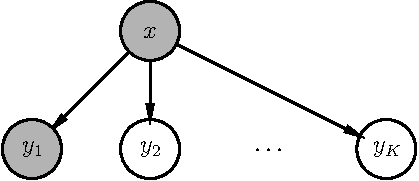
\includegraphics[width=.8\textwidth]{mmclassifier.pdf} % textwidth in subfigure environment
        \caption{Multi-class multi-label classifier}
    \end{subfigure}
    \begin{subfigure}[t]{.33\textwidth}
        \centering
        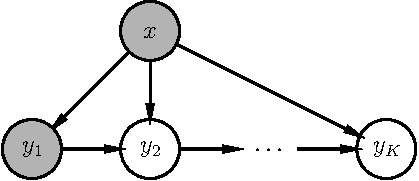
\includegraphics[width=.8\textwidth]{memm.pdf}
        \caption{MEMM}
    \end{subfigure}
    \begin{subfigure}[t]{.33\textwidth}
        \centering
        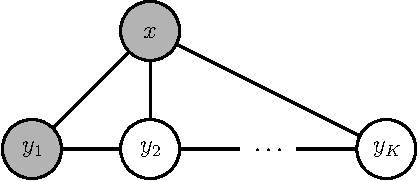
\includegraphics[width=.8\textwidth]{crf.pdf}
        \caption{CRF}
    \end{subfigure}
    \caption{Graphical models for trajectory recommendation.}
    \label{fig:pgm}
\end{figure}


\subsubsection{Maximum-entropy Markov models}
\label{sec:memm}

For MEMM, the compatibility function $f(\mathbf{x}, \mathbf{y})$ is the probability of trajectory $\mathbf{y}$ given query $\mathbf{x} = (s, K)$,
\begin{equation*}
f(\mathbf{x}, \mathbf{y}) 
= \mathbb{P}(\mathbf{y} \mid \mathbf{x}; \mathbf{w}) 
= \mathbb{P}(y_1 \mid \mathbf{x}; \mathbf{w}) \cdot \prod_{j=2}^K \mathbb{P}(y_j \mid y_{j-1}, \mathbf{x}; \mathbf{w})
= 1 \cdot \prod_{j=2}^{K}~
  \frac{\exp \left(\mathbf{w}^\top \Psi_j(\mathbf{x}, y_{j-1}, y_j) \right)}
       {\sum_{y' \in \mathcal{P}} \exp \left(\mathbf{w}^\top \Psi_j(\mathbf{x}, y_{j-1}, y') \right)},
\end{equation*}
where we do local normalisation.

The negative log-likelihood of training set is
\begin{equation*}
\ell(\mathbf{w}) 
= -\sum_{i=1}^N \log \mathbb{P}(\mathbf{y}^{(i)} \mid \mathbf{x}^{(i)}; \mathbf{w}) \\
= -\sum_{i=1}^N \sum_{j=2}^{\mid \mathbf{y}^{(i)} \mid} 
                \mathbf{w}^\top \Psi_j(\mathbf{x}^{(i)}, y_{j-1}^{(i)}, y_j^{(i)}) +
   \sum_{i=1}^N \sum_{j=2}^{\mid \mathbf{y}^{(i)} \mid} 
                \log \sum_{y' \in \mathcal{P}} \exp \left(\mathbf{w}^\top \Psi_j(\mathbf{x}^{(i)}, y_{j-1}^{(i)}, y') \right).
\end{equation*}

To learn the parameters, we maximise the likelihood of training set by minimising its negative log-likelihood (with L2 regularisation)
\begin{equation}
\label{eq:trainmemm}
\min_{\mathbf{w}} \frac{1}{2} \mathbf{w}^\top \mathbf{w} + C \ell(\mathbf{w}).
\end{equation}

A straightforward approach to optimise the above objective is employing gradient descent. 
Let $J(\mathbf{w})$ be the objective (cost function), i.e.,
\begin{align*}
J(\mathbf{w}) 
&= \frac{1}{2} \mathbf{w}^\top \mathbf{w} + C \ell(\mathbf{w}) \\
&= \frac{1}{2} \mathbf{w}^\top \mathbf{w} -
   C \sum_{i=1}^N \sum_{j=2}^{\mid \mathbf{y}^{(i)} \mid} \mathbf{w}^\top \Psi_j(\mathbf{x}^{(i)}, y_{j-1}^{(i)}, y_j^{(i)}) +
   C \sum_{i=1}^N \sum_{j=2}^{\mid \mathbf{y}^{(i)} \mid} \log \sum_{y' \in \mathcal{P}} 
     \exp \left(\mathbf{w}^\top \Psi_j(\mathbf{x}^{(i)}, y_{j-1}^{(i)}, y') \right).
\end{align*}
The gradient of the cost function w.r.t. parameters $\mathbf{w}$ is
\begin{align*}
\frac{\partial J{\mathbf{w}}}{\partial \mathbf{w}}
&= \mathbf{w} + C \frac{\partial \ell(\mathbf{w})}{\partial \mathbf{w}} \\
&= \mathbf{w} - C \sum_{i=1}^N \sum_{j=2}^{\mid \mathbf{y}^{(i)} \mid} \Psi_j(\mathbf{x}^{(i)}, y_{j-1}^{(i)}, y_j^{(i)}) +
   C \sum_{i=1}^N \sum_{j=2}^{\mid \mathbf{y}^{(i)} \mid} 
     \frac{\sum_{y' \in \mathcal{P}} \left( \Psi_j(\mathbf{x}^{(i)}, y_{j-1}^{(i)}, y') \cdot 
           \exp \left(\mathbf{w}^\top \Psi_j(\mathbf{x}^{(i)}, y_{j-1}^{(i)}, y') \right) \right)}
          {\sum_{y' \in \mathcal{P}} \exp \left(\mathbf{w}^\top \Psi_j(\mathbf{x}^{(i)}, y_{j-1}^{(i)}, y') \right)}.
\end{align*}


MEMM is a directed graphical model (as shown in Figure~\ref{fig:pgm}(b)) which captures transitions from one POI to any other POIs simultaneously, 
in contrast, pairwise ranking (Section~\ref{sec:rank}) captures only pairwise relations independently.

To make a prediction, we need to do a MAP inference (which can be done using the Viterbi algorithm if duplicated POIs are permitted)
\begin{equation}
\label{eq:testmemm}
\begin{aligned}
\mathbf{y}^* 
&= \argmax_{\mathbf{y} \in \mathcal{Y}_\mathbf{x}}~f(\mathbf{x}, \mathbf{y})
 = \argmax_{\mathbf{y} \in \mathcal{Y}_\mathbf{x}}~\mathbb{P}(\mathbf{y} \mid \mathbf{x}; \mathbf{w})
 = \argmax_{\mathbf{y} \in \mathcal{Y}_\mathbf{x}}~\log \mathbb{P}(\mathbf{y} \mid \mathbf{x}; \mathbf{w}) \\
&= \argmax_{\mathbf{y} \in \mathcal{Y}_\mathbf{x}}~\sum_{j=2}^{K} \mathbf{w}^\top \Psi_j(\mathbf{x}, y_{j-1}, y_j) - 
   \sum_{j=2}^{K} \log \sum_{y' \in \mathcal{P}} \exp \left(\mathbf{w}^\top \Psi_j(\mathbf{x}, y_{j-1}, y') \right).
\end{aligned}
\end{equation}

Furthermore, we can explicitly model dependencies between POIs in trajectory by adding dependences between variable $y_j$ and $y_k,~ j < k$,
which results in another compatibility function
\begin{equation*}
f(\mathbf{x}, \mathbf{y}) 
= \mathbb{P}(\mathbf{y} \mid \mathbf{x}; \mathbf{w}) 
= \mathbb{P}(y_1 \mid \mathbf{x}; \mathbf{w}) \cdot \prod_{j=2}^K \mathbb{P}(y_j \mid y_1,\dots, y_{j-1}, \mathbf{x}; \mathbf{w})
= 1 \cdot \prod_{j=2}^{K}~
  \frac{\exp \left(\mathbf{w}_j^\top \Psi_j(\mathbf{x}, y_1, \dots, y_{j-1}, y_j) \right)}
       {\sum_{y' \in \mathcal{P}} \exp \left(\mathbf{w}_j^\top \Psi_j(\mathbf{x}, y_1, \dots, y_{j-1}, y') \right)}.
\end{equation*}

It can be trained similarly using the maximum likelihood principle.



\subsubsection{Conditional random fields}
\label{sec:crf}

For linear chain CRF, the compatibility function $f(\mathbf{x}, \mathbf{y})$ is also the probability of trajectory $\mathbf{y}$ given
query $\mathbf{x} = (s, K)$,
\begin{equation*}
f(\mathbf{x}, \mathbf{y}) = \mathbb{P}(\mathbf{y} \mid \mathbf{x}; \mathbf{w}) 
= \frac{\exp \left( \mathbf{w}^\top \Psi(\mathbf{x}, \mathbf{y}) \right)}
       {\sum_{\mathbf{y}' \in \mathcal{Y}_\mathbf{x}} \exp \left( \mathbf{w}^\top \Psi(\mathbf{x}, \mathbf{y}') \right)}
= \frac{\prod_{j=2}^{K} \exp \left( \mathbf{w}_j^\top \Psi_j(\mathbf{x}, y_{j-1}, y_j) \right)}
       {\sum_{\mathbf{y}' \in \mathcal{Y}_\mathbf{x}} \prod_{j=2}^{K} \exp \left( \mathbf{w}_j^\top \Psi_j(\mathbf{x}, y_{j-1}', y_j') \right)},
\end{equation*}
where $\mathbf{y} \in \mathcal{Y}_\mathbf{x}$ and we assume decomposition 
$\mathbf{w}^\top \Psi(\mathbf{x}, \mathbf{y}) = \sum_{j=2}^{K} \mathbf{w}_j^\top \Psi_j(\mathbf{x}, y_{j-1}, y_j)$.
The denominator is known as the \emph{partition function} and we do global normalisation.

The negative log-likelihood of training set is
\begin{equation*}
\ell(\mathbf{w}) 
= -\sum_{i=1}^N \log \mathbb{P}(\mathbf{y}^{(i)} \mid \mathbf{x}^{(i)}; \mathbf{w})
= -\sum_{i=1}^N \sum_{j=2}^{\mid \mathbf{y}^{(i)} \mid} \mathbf{w}_j^\top \Psi_j(\mathbf{x}^{(i)}, y_{j-1}^{(i)}, y_j^{(i)}) +
   \sum_{i=1}^N \log \sum_{\mathbf{y}' \in \mathcal{Y}_\mathbf{x}} 
                \prod_{j=2}^{K} \exp \left(\mathbf{w}_j^\top \Psi_j(\mathbf{x}^{(i)}, y_{j-1}', y_j')\right).
\end{equation*}

To learn the parameters, we maximise the likelihood of training set by minimising its negative log-likelihood (with L2 regularisation)
\begin{equation}
\label{eq:traincrf}
\min_{\mathbf{w}} \frac{1}{2} \mathbf{w}^\top \mathbf{w} + C \ell(\mathbf{w}).
\end{equation}

CRF is an undirected graphical model as shown in Figure~\ref{fig:pgm}(c).
Similar to MEMM, CRF can capture transitions from one POI to any other POIs simultaneously.
To make a prediction, we need to do a MAP inference
\begin{equation}
\label{eq:testcrf}
\begin{aligned}
\mathbf{y}^* 
&= \argmax_{\mathbf{y} \in \mathcal{Y}_\mathbf{x}}~f(\mathbf{x}, \mathbf{y})
 = \argmax_{\mathbf{y} \in \mathcal{Y}_\mathbf{x}}~\mathbb{P}(\mathbf{y} \mid \mathbf{x}; \mathbf{w})
 = \argmax_{\mathbf{y} \in \mathcal{Y}_\mathbf{x}}~\log \mathbb{P}(\mathbf{y} \mid \mathbf{x}; \mathbf{w}) \\
&= \argmax_{\mathbf{y} \in \mathcal{Y}_\mathbf{x}}~\sum_{j=2}^{K} \mathbf{w}_j^\top \Psi_j(\mathbf{x}, y_{j-1}, y_j) -
   \log \sum_{\mathbf{y}' \in \mathcal{Y}_\mathbf{x}} \prod_{j=2}^{K} \exp \left( \mathbf{w}_j^\top \Psi_j(\mathbf{x}, y_{j-1}', y_j') \right).
\end{aligned}
\end{equation}

\eat{TODO: why people usually employ CRF?}


\subsubsection{Structured SVM}
\label{sec:ssvm}

For structured SVM, the compatibility function $f(\mathbf{x}, \mathbf{y})$ is this linear form,
\begin{equation*}
f(\mathbf{x}, \mathbf{y}) = \mathbf{w}^\top \Psi(\mathbf{x}, \mathbf{y}),
\end{equation*}
where $\Psi(\mathbf{x}, \mathbf{y})$ is a \emph{joint feature map} 
that captures features extracted from both query $\mathbf{x}$ and trajectory $\mathbf{y}$.

The design of joint feature $\Psi(\cdot,\cdot)$ is problem specific, 
for trajectory recommendation, we assume decomposition
\begin{equation*}
\label{eq:jointfeature}
\mathbf{w}^\top \Psi(\mathbf{x}, \mathbf{y}) 
= \sum_{j=2}^{\mid \mathbf{y} \mid} 
  \left( \mathbf{w}_j^\top \Psi_j(\mathbf{x}, y_j) + 
  \mathbf{w}_{j-1,j}^\top \Psi_{j-1, j}(\mathbf{x}, y_{j-1}, y_j) \right),
\end{equation*}
where $\Psi_j$ is a feature vector of POI $y_j$ (w.r.t. query $\mathbf{x}$)
and $\Psi_{j-1,j}$ is a pairwise feature vector that captures the affinity of transition from POI $y_{j-1}$ to POI $y_j$.

To learn the parameters, we train the structured SVM by optimising a quadratic program (QP),
\begin{equation}
\label{eq:nslack}
\begin{aligned}
\min_{\mathbf{w}, ~\bm{\xi} \ge 0} ~& \frac{1}{2} \mathbf{w}^\top \mathbf{w} + \frac{C}{n} \sum_{i=1}^n \xi_i \\
s.t.~~ ~& \mathbf{w}^\top \Psi(\mathbf{x}^{(i)}, \mathbf{y}^{(i)}) - \mathbf{w}^\top \Psi(\mathbf{x}^{(i)}, \bar{\mathbf{y}}) \ge 
       \Delta(\mathbf{y}^{(i)}, \bar{\mathbf{y}}) - \xi_i, ~\bar{\mathbf{y}} \in \mathcal{Y}_{\mathbf{x}^{(i)}},~\forall i,
\end{aligned}
\end{equation}
where $\Delta(\mathbf{y}, \bar{\mathbf{y}})$ is a discrepancy function that measures the loss 
for predicting $\bar{\mathbf{y}}$ given ground truth $\mathbf{y}$, 
and slack variable $\xi_i$ is the \emph{hinge loss} for the prediction of the $i$-th example~\cite{tsochantaridis2005large},
\begin{equation*}
\xi_i = \max \left( 0,~ 
        \max_{\bar{\mathbf{y}} \in \mathcal{Y}_{\mathbf{x}^{(i)}}} 
        \left\{ \Delta(\mathbf{y}^{(i)}, \bar{\mathbf{y}}) + \mathbf{w}^\top \Psi(\mathbf{x}^{(i)}, \bar{\mathbf{y}}) \right\} -
        \mathbf{w}^\top \Psi(\mathbf{x}^{(i)}, \mathbf{y}^{(i)}) \right).
\end{equation*}
%This formulation is called "$n$-slack" as we have one slack variable for each example in training set.

We can rewrite the constraint in problem (\ref{eq:nslack}) as
\begin{equation}
\label{eq:ssvminf}
\mathbf{w}^\top \Psi(\mathbf{x}^{(i)}, \mathbf{y}^{(i)}) + \xi_i \ge
          \max_{\bar{\mathbf{y}} \in \mathcal{Y}_{\mathbf{x}^{(i)}}}
          \left\{\mathbf{w}^\top \Psi(\mathbf{x}^{(i)}, \bar{\mathbf{y}}) + \Delta(\mathbf{y}^{(i)}, \bar{\mathbf{y}}) \right\},~ \forall i,
\end{equation}
where the right hand side is known as the \emph{loss-augmented inference}.

To solve problem (\ref{eq:nslack}), one option is simply enumerating all constraints, and feeding the problem into a standard QP solver.
However, this approach is impractical as there is a constraint for every possible label $\bar{\mathbf{y}}$.
Instead, we use a cutting-plane algorithm which repeatedly solves QP (\ref{eq:nslack}) 
w.r.t. different set of constraints~\cite{joachims2009predicting}.
In each iteration, a new constraint is formed by solving the loss-augmented inference, 
which helps shrink the feasible region of the problem.



\subsubsection{Discussion}

All structured models described above suffer from a number of drawbacks.
\begin{enumerate}
\item The MEMM model (Section~\ref{sec:memm}) is relatively easy to train, 
      but the inference (Equation~\ref{eq:testmemm}) will not retain its efficiency if the no duplicates constraints are required.
\item The CRF model (Section~\ref{sec:crf}) suffers from inefficient training (Equation~\ref{eq:traincrf}) and 
      inference (Equation~\ref{eq:testcrf}) as the partition function cannot be computed efficiently.
\item Both the loss-augmented inference and prediction inference for structured SVM (Section~\ref{sec:ssvm}) cannot be done efficiently 
      if the no duplicates constraints are required.
\end{enumerate}

Approximate inference methods are critical for MEMM and CRF.
On the other hand, inference in structured SVM is equivalent to 
find a maximum-weight loop-less path with exactly $K$ edges in a complete weighted (both nodes and edges) graph, which is NP-hard (proof?).
Possible solutions including 
\begin{itemize}
\item formulating it as an integer linear program (ILP) and solve it using an ILP solver, 
      or using lazy constraint generation/cutting-plane techniques with a LP solver;
\item in addition, we can employ the list Viterbi algorithm~\cite{nilsson2001sequentially,seshadri1994list} 
      which sequentially find the next best (scored) trajectory until a maximum-weight loop-less path with exactly $K$ edges is found;
\item moreover, we can employ heuristics such as greedy search or the Christofides algorithm~\cite{christofides1976} 
      when the problem has the triangle inequality property (for trajectories, indeed).
\end{itemize}
These options are applicable to MEMM (Section~\ref{sec:memm}) as well.



\subsubsection{Inference algorithms}
\label{sec:inference}

\paragraph{Integer linear program}
If we formulate an ILP to do inference and employ the sub-tour elimination constraints from TSP, we have
\begin{alignat}{5}
& \max_{u,v} ~&& \sum_{k=1}^M \mathbf{w}_k^\top \phi_k(\mathbf{x}, p_k) \sum_{j=1}^M u_{jk} + 
                 \sum_{j=1}^M \sum_{k=1}^M u_{jk} \mathbf{w}_{jk}^\top \phi_{j, k}(\mathbf{x}, p_j, p_k) \\
& s.t. ~~ ~&& u_{jk}, ~z_j \in \{0, 1\}, ~u_{jj}=0, ~z_1=0, ~v_j \in \mathbf{Z},~ p_j \in \mathcal{P}, ~\forall j, k = 1,\cdots,M   \label{eq:cons1} \\
&          && \sum_{k=2}^M u_{1k} = 1, ~\sum_{j=2}^M u_{j1} = 0  \label{eq:cons2} \\
&          && \sum_{j=1}^M u_{jl} = z_l + \sum_{k=2}^M u_{lk} \le 1,   ~\forall l=2,\cdots,M                    \label{eq:cons3} \\
&          && \sum_{j=1}^M \sum_{k=1}^M u_{jk} = L-1,                                                           \label{eq:cons4} \\
&          && v_j - v_k + 1 \le (M-1) (1-u_{jk}),                     \forall j,k=2,\cdots,M                    \label{eq:cons5}
\end{alignat}
where $u_{jk}$ is a binary decision variable that determines whether the transition from $p_j$ to $p_k$ is in the resulting trajectory,
$z_j$ is a binary decision variable that determines whether $p_j$ is the last POI in trajectory.
$L$ is the number of POIs in trajectory.
For brevity, we arrange the POIs such that $p_1 = s$.
Firstly, the desired trajectory should start from $s$ (Constraint~\ref{eq:cons2}).
In addition, any POI could be visited at most once (Constraint~\ref{eq:cons3}).
Moreover, only $L-1$ transitions between POIs are permitted (Constraint~\ref{eq:cons4}),
i.e., the number of POI visits should be exactly $L$ (including $s$).
The last constraint, where $v_i$ is an auxiliary variable,
enforces that only a single sequence of POIs without sub-tours is permitted in the trajectory.

If we employ the above ILP to do loss-augmented inference, we can simply add a linear loss function to the objective, 
e.g., $\Delta(\mathbf{y}, \bar{\mathbf{y}}) = 1 - \sum_{j=1}^M \sum_{k=1}^M u_{j, y_k}$ if we define the loss as the number of mispredicted POIs,
where $\mathbf{y}$ is the ground truth and $\bar{\mathbf{y}}$ is the trajectory corresponding to the optimal solution of this ILP.

\paragraph{The list Viterbi algorithm}
Instead of employ an algorithm with exponential time complexity (e.g., ILP) to do inference,
we can resort to an iterative algorithm such as the list Viterbi algorithm~\cite{nilsson2001sequentially,seshadri1994list}
which sequentially find the $k$-th best (scored) trajectory given the best, $2$nd best, \dots, $(k-1)$-th best (scored) trajectories,
as described in Algorithm~\ref{alg:listviterbi}.


\begin{algorithm}[htbp]
\caption{The list Viterbi algorithm for inference}
\label{alg:listviterbi}
\begin{algorithmic}[1]
\STATE \textbf{Input}: $\mathbf{x}=(s, K),~ \mathcal{P},~ \mathbf{w},~ \Psi$
\STATE Initialise score matrices $\alpha,~ \beta,~ f_t,~ f_{t, t+1}$, a max-heap $H,~ k=0$.
\STATE $\triangleright$ Do the forward-backward procedure~\cite{rabiner1989tutorial}
\STATE $\forall p_j \in \mathcal{P},~ \alpha_t(p_j) = 
        \begin{cases}
        0,~ t = 1 \\
        \max_{p_i \in \mathcal{P}} \left\{ \alpha_{t-1}(p_i) + \mathbf{w}_{ij}^\top \Psi_{ij}(\mathbf{x}, p_i, p_j) + 
        \mathbf{w}_j^\top \Psi_j(\mathbf{x}, p_j) \right\},~ t=2,\dots,K
        \end{cases}$

\STATE $\forall p_i \in \mathcal{P},~ \beta_t(p_i) = 
        \begin{cases}
        0,~ t = K \\
        \max_{p_j \in \mathcal{P}} \left\{ \mathbf{w}_{ij}^\top \Psi_{ij}(\mathbf{x}, p_i, p_j) + 
        \mathbf{w}_j^\top \Psi_j(\mathbf{x}, p_j) + \beta_{t+1}(p_j) \right\},~ t = K-1,\dots,1
        \end{cases}$

\STATE $\forall p_i \in \mathcal{P},~ f_t(p_i) = \alpha_t(p_i) + \beta_t(p_i),~ t = 1,\dots,K$
\STATE $\forall p_i, p_j \in \mathcal{P},~ f_{t,t+1}(p_i, p_j) = \alpha_t(p_i) + \mathbf{w}_{ij}^\top \Psi_{ij}(\mathbf{x}, p_i, p_j) + 
                              \mathbf{w}_j^\top \Psi_j(\mathbf{x}, p_j) + \beta_{t+1}(p_j),~ t = 1,\dots,K-1$

\STATE $\triangleright$ Identify the best (scored) trajectory $\mathbf{y}^1=(y_1^1,\dots,y_K^1)$ (possibly with sub-tours)
\STATE $y_t^1 = \begin{cases}
                s,~ t = 1 \\
%                \argmax_{p \in \mathcal{P}} \left\{ f_{1,2}(s, p) \right\},~ t = 2, \\
                \argmax_{p \in \mathcal{P}} \left\{ f_{t-1,t}(y_{t-1}^1, p) \right\},~ t = 2,\dots,K
                \end{cases}$

\STATE $r^1 = \max_{p \in \mathcal{P}} \left\{ f_K(p) \right\}~~~ \triangleright$ $r^1$ is the score/priority of $\mathbf{y}^1$
\STATE $H.\textit{push}\left(r^1,~ (\mathbf{y}^1, \textsc{nil}, \emptyset) \right)$

\WHILE{$H \ne \emptyset$ \textbf{and} $k < \,\mid\!\!\mathcal{P}\!\!\mid^{K-1} - \prod_{t=2}^K (\mid\!\!\mathcal{P}\!\!\mid-t+1)$}
    \STATE $r^k,~ (\mathbf{y}^k, I, S) = H.\textit{pop}()~~~ \triangleright$ 
           $r^k$ is the score of $\mathbf{y}^k=(y_1^k,\dots,y_K^k)$, $I$ is the partition index, and $S$ is the exclude set
    \STATE $k = k + 1$
    \RETURN $\mathbf{y}^k$ if NO sub-tours in $\mathbf{y}^k$
    \STATE $\bar{I} = \begin{cases}
                      2,~ I = \textsc{nil} \\
                      I,~ \text{otherwise}
                      \end{cases}$

    \FOR{$t = \bar{I},\dots,K$}
        \STATE $\bar{S} = \begin{cases}
                          S \cup \{ y_t^k \},~ t = \bar{I} \\
                          \{ y_t^k \},~ \text{otherwise}
                          \end{cases}$

        \STATE $\bar{y}_j = \begin{cases}
                            y_j^k,~~ j=1,\dots,t-1 \\
                            %\argmax_{p \in \mathcal{P} \setminus \textit{new\_exclude\_set}} f_{t-1,t}(y_{t-1}^k, p),~ j=t \\
                            \argmax_{p \in \mathcal{P} \setminus \bar{S}} \left\{ f_{t-1,t}(y_{t-1}^k, p) \right\},~ j=t \\
                            \argmax_{p \in \mathcal{P}} \left\{ f_{j-1, j}(\bar{y}_{j-1}, p) \right\},~ j=t+1,\dots,K
                \end{cases}$
        \STATE $\bar{r} = \begin{cases}
                          f_{t-1,t}(y_{t-1}^k, \bar{y}_t),~ I = \textsc{nil} \\
                          r^k + f_{t-1,t}(y_{t-1}^k, \bar{y}_t) - f_{t-1,t}(y_{t-1}^k, y_t^k),~ \text{otherwise}
                          \end{cases}$

        $H.\textit{push}\left(\bar{r}, (\bar{\mathbf{y}}, t, \bar{S}) \right)$
    \ENDFOR
\ENDWHILE
\end{algorithmic}
\end{algorithm}



\eat{
\subsection{Other models}
\label{sec:other}
Label ranking model,
Plackett-Luce probabilistic ranking
}


\section{Features}
\label{sec:feature}

\eat{
\underline{REVISE FEATURE DESIGN}
}

The POI and query specific features extracted from trajectories are shown in Table~\ref{tab:poifeature},
features that describe the transition preference between different POIs are shown in Table~\ref{tab:tranfeature}.



\begin{table*}[ht]
\caption{Features of POI $p$ with respect to query $(s,K)$}
\label{tab:poifeature}
\centering
\setlength{\tabcolsep}{10pt} % tweak the space between columns
\begin{tabular}{l|l} \hline
\textbf{Feature}  & \textbf{Description} \\ \hline
\texttt{category}               & one-hot encoding of the category of $p$ \\
\texttt{neighbourhood}          & one-hot encoding of the POI cluster that $p$ resides in \\
\texttt{popularity}             & logarithm of POI popularity of $p$ \\
\texttt{nVisit}                 & logarithm of the total number of visit by all users at $p$ \\
\texttt{avgDuration}            & logarithm of the average duration at $p$ \\ \hline

%\texttt{nOccurrence}            & the number of times $p$ occurred in a trajectory that satisfies the query \\ DON'T know given new query

\texttt{trajLen}                & trajectory length $K$, i.e., the number of POIs required \\
\texttt{sameCatStart}           & $1$ if the category of $p$ is the same as that of $s$, $-1$ otherwise \\
\texttt{sameNeighbourhoodStart} & $1$ if $p$ resides in the same POI cluster as $s$, $-1$ otherwise \\
\texttt{distStart}              & distance between $p$ and $s$, calculated using the Haversine formula \\
\texttt{diffPopStart}           & real-valued difference in POI popularity of $p$ from that of $s$ \\
\texttt{diffNVisitStart}        & real-valued difference in the total number of visit at $p$ from that at $s$ \\
\texttt{diffDurationStart}      & real-valued difference in average duration at $p$ from that at $s$ \\
\hline
\end{tabular}
\end{table*}



\begin{table}[ht]
\caption{POI features used to estimate the (feature-wise) transition probabilities}
\label{tab:tranfeature}
\centering
%\setlength{\tabcolsep}{28pt} % tweak the space between columns
\begin{tabular}{l|l} \hline
\textbf{Feature}       & \textbf{Description} \\ \hline
\texttt{category}      & category of POI \\
\texttt{neighbourhood} & the cluster that a POI resides in \\
\texttt{popularity}    & (discretised) popularity of POI \\
\texttt{nVisit}        & (discretised) total number of visit at POI \\
\texttt{avgDuration}   & (discretised) average duration at POI \\ \hline
\end{tabular}
\end{table}



\bibliographystyle{ieeetr}
\bibliography{ref}

\end{document}
